\section{Implementation and experiments}
In this chapter the results of all experiments performed for predicting fluorescence signal from 4 cell oganelles: nuclei, endoplaspic reticulum, Golgi apparatus, and full cell fluorescence are provided and discussed. It starts first with a description of the models and data used in the experiments, followed by 4 subsections dedicated to each of the organelles. Each subsection describes its own different approaches in, for example, pre- or postprocessing needed, difficulties that occured during preparation or training steps and well as results obtained for each organelle separately. At the end of this chapter an alternative way of the models performance estimation is provided, which is very important for the practical application of them.

    \subsection{Model training}
    \subsubsection{Neural network architecture}
        As was described in section \ref{subsection:dl} the choice of the model architecture fell onto the UNet. Here will be provided a detailed decription of the architecture and the different layers used. An architecture used in this research was chosen based on paper [TODO LaChance]. The input to this network is a $256 \times 256$-pixel DIC image that should be already preprocessed with the corresponding to the desired organelle preprocessing pipeline. Specifications about different preprocessings are described separately in the separate subsections of different organelles.

The encoder part of the UNet (Figure \ref{fig:unet}) step by step compresses spatial dimensions of the image (the spatial dimension size is detoned by a number on the left of each green block) into tensors or feature maps with an increasing amount of filters (filters are denoted by a number on the top of each green block). This allows to reduce the spatial information in the image and capture semantics. Decoder part on the contrary decompresses feature maps gradually increasing the amount of spatial information in tensors and reducing the number of filters. All convolutional layers use convolution of size $3 \times 3$ with the corresponding number of filters that are denoted in the Figure. Downsapling in encoder reduces the spatial dimension twice during each step and implemented using max-pooling with a size of $2 \times 2$. Upsampling in decoder increases the spatial dimension also twice during each step and implemented using transposed convolution with a size of $2 \times 2$. After the first convolution layer after each max-pooling step a batch normalization layer was used as they are well-known for speeding up the training process [cite Ioffe]. One should not forget though that using batch normalization might be sometimes dangerous due to the leak of information [cite Fetterman 2020]. Additionally dropouts were used for example for actin predictions as the model would encounter overfit quite easily there, however for default choice dropouts were not pressent. That is another thing that differs this architecture from the original in [TODO Cite LaChance] paper. The last layer of the UNet is a sigmoid activation function.
\begin{figure}[htb]
	\begin{center}
		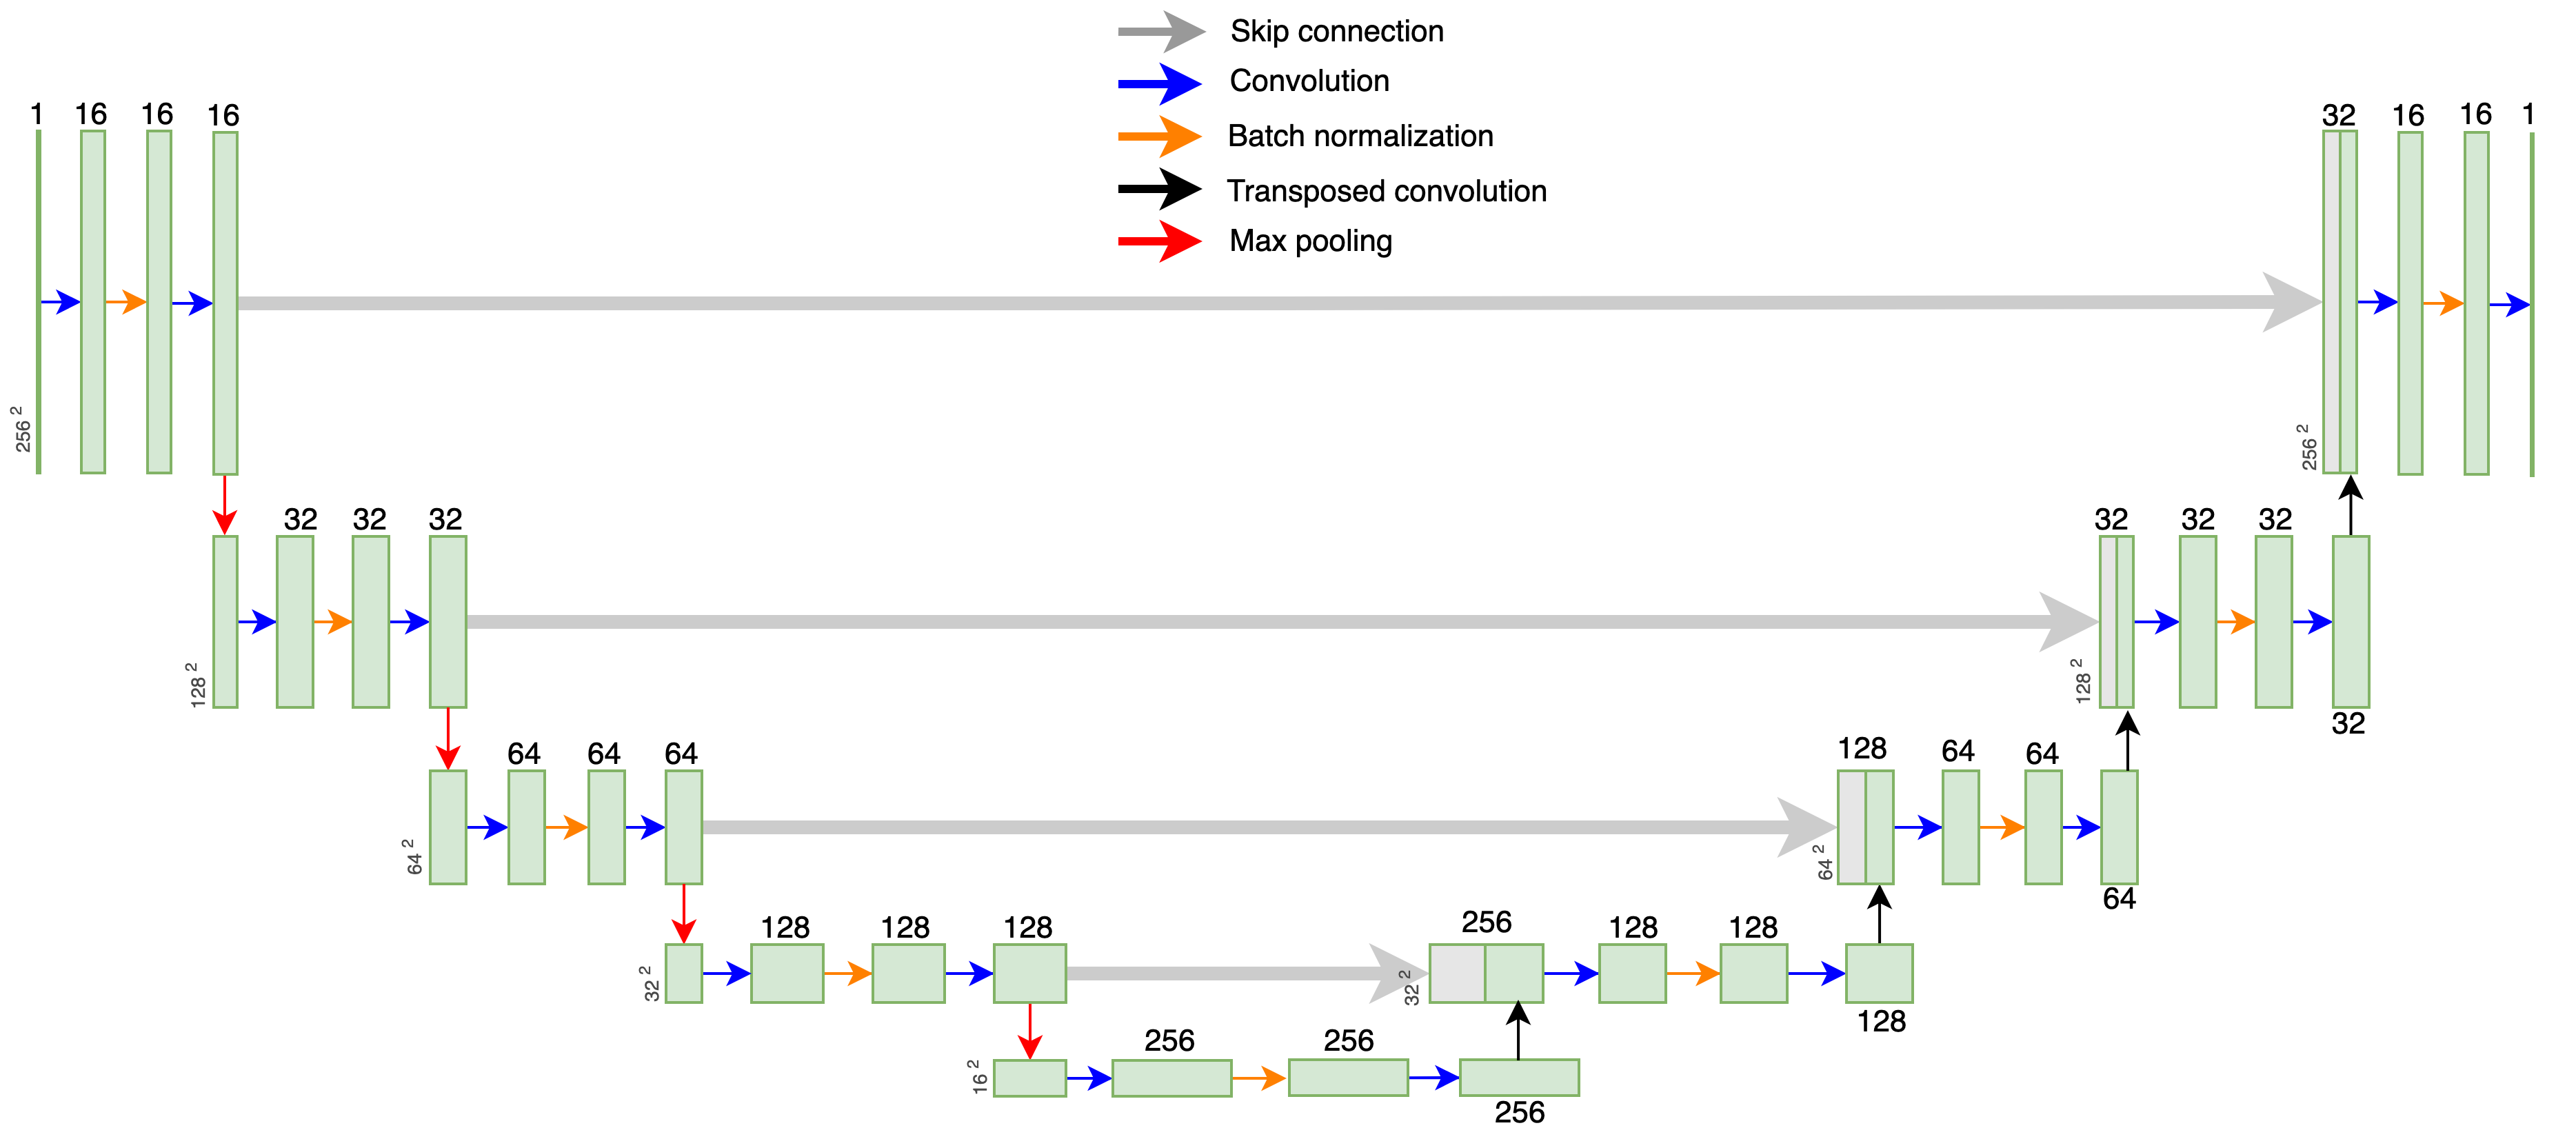
\includegraphics[width=\linewidth]{bilder/Unet.png}
		\caption{Unet}\label{fig:unet}
	\end{center}
\end{figure}

There is a space for potential improvements regarding the model architecture here: for example, [Shiyui 2021] recommends to use special dense-block after each convolutional layer that would consist of another 3 convolutional layers with 24 filters, Batch normalization layer and ReLU activations each. This could potentially facilitate efficient training of the model, still most probably the efficience comes mostly from Batch normalization layers that are already used in our architecture. Nethertheless the idea of using the bigger model as [Shiyui 2021], more specifically using more filters, indeed improves the predictions as it will be explained in Section [TODO ref section]. That leaves the plave available for further research and improvements regarding the size of the model and the additionally used dense-blocks. 

An interesting question that automatically rises here is what do embeddings (output tensors from the encoder) represent. There is a big difference between any representation learning network such as an autoencoder and a UNet - a UNet model uses skip-connections that allow to propagate an information between its encoder and a decoder. Meaning that embeddings do not contain purely semantic information, because essentially the network is not pushed to compress the information severely (as autoencoder would do), but it should only to extract relevant for segmentation features. One of the questions solved in this work was wether or not UNet embeddings are clustering based on the following classes: cell phenotypes, any kind of corruption within the data. For example, it would be bery usefull to be able to not only predict the data itselt, but also to say wethere the prediction is reliable of not. The initial hypothesis here would be that if the predictions are not of a good enough quality this would also be reflected in the embeddings. 
    \subsubsection{Available data}
        Description of the datasets and the amount of images in each category.

\begin{table}[H]
    \centering
    \caption{Available data for each fo the organelles}
        \begin{adjustbox}{width=0.7\textwidth}
            \begin{tabular}{|c||c|c|c|c|}\hline
                &Total images
                &Training crops
                &Validation crops
                &Test crops
                \\\hline\hline
                Nuclei &595&27,264&3,008&7,616\\\hline
                Actin &400&18,432&2,048&5120\\\hline
                Golgi &761&23,036&2,336&6,347\\\hline
                H19 &400&27,264&3,008&7,61\\\hline
                Nucleolei &?&?&?&?\\\hline
            \end{tabular}
        \end{adjustbox}
\end{table}

    \subsubsection{Training costs estimation}
        For training purposes in this research cloud computing services were used, or more specifically - Amazon Web Services (AWS). These remotely located servers provide an possibility to train your models on a variety of graphic cards paying for minute rate. In order to keep the costs unter the control it was important to estimate the time needed for training in advance to choose the most efficient GPU possible.

Cost estimation is additionally important for the model inference as well during the production. Although for production purposes the lambda functions from AWS can used, then are triggered only when the inference request arrives and are turned off automatically shortly after.

For both training an inference purposes two GPU models were tested g3-4xlarge which is an NVIDIA Tesla M60 and p3-2xlarge which is a NVIDIA Tesla V100. The datasets on which the experiments were performed on were a nuclei training and validation dataset. The resulting costs are presented in the Tables \ref{table:costs-training}, \ref{table:costs-inference}.

\begin{table}[H]
    \centering
    \caption{Costs estimations of AWS use for training models}
        \begin{adjustbox}{width=0.7\textwidth}
            \begin{tabular}{|c||c|c|c|c|}\hline
                &Runtime (1 epoch)
                &Dataset size
                &Costs per minute
                &Cost per epoch
                \\\hline\hline
                g3.4xlarge & $6.5 mins$ & $18,432$ & $0.07125\$$ & $0.3$\\\hline
                p3.2xlarge & $400$ & $18,432$ & $0.1911\$$ &$0.18$\\\hline
            \end{tabular}
        \end{adjustbox}
    \label{table:costs-training}
\end{table}

%g3 391, 261, 260
%p3 170, 57, 56


\begin{table}[H]
    \centering
    \caption{Costs estimations of AWS use for inference purposes}
        \begin{adjustbox}{width=0.7\textwidth}
            \begin{tabular}{|c||c|c|c|c|}\hline
                &Runtime
                &Dataset size
                &Costs per minute
                &Cost of inference
                \\\hline\hline
                g3.4xlarge & $?\text{mins}$ & $2,048$ & $0.07125$ & $? \$$\\\hline
                p3.2xlarge & $?\text{mins}$ &  $2,048$ & $0.1911$ &$? \$$\\\hline
            \end{tabular}
        \end{adjustbox}
    \label{table:costs-inference}
\end{table}

As a conclusion even though a p3 instance seems to be much more expensive, it is also much more efficient and the costs estimated to training times are lower. That is why all the training experiments in this research were conducted on an NVIDIA Tesla V100 GPU.
    \subsubsection{Augmentations}
        \label{section:augmentations}
        Augmentations are a powerful regularization technique that helps the network to generalize better [cite Wang 2017] and is an effective solution for a situation with the lack of labeled data [cite Yang 2022]. The main idea behind augmentation is to increase the diversity of training data, when the acquisition of the real training data is expensive. Augmenting existing images creates the new synthetic samples which are hypothetically very close to the original true distribution of images. However, one should be very cautios regarding the type of augmentations that can be used. Augmentation must enrich the dataset, but it should not change the semantics hidden in each image. The peculiarity of current research is the pair-wise correspondence between the DIC input and the output fluorescence. One should not change the input in such a way that the fluorescence signal could not be inferred from it. Therefore the following augmentations have been used on cropped images:

\begin{itemize}
	\item \textbf{Flipping}: Flip the crop horizontally (30\% chance), vertically (30\% chance) or both.
	\item \textbf{Random rotation}: Rotates the crop by a random angle.
	\item \textbf{Random scaling}: Reduces crop size by 100 (20\% chance), 50 (20\% chance) or 20 (60\% chance) pixels from each side (down, top, left, right).
	\item \textbf{Contrast}: Halves an image's constrast (50\% chance), or triples it (50\% chance). Applied with a 20\% chance.
	\item \textbf{Defocus blur}: Imitates a defocus blur of severity level 4 (see section [TODO cite section]) on an image with a 20\% chance.
\end{itemize}

\paragraph{Special augmentations for rotation and scaling}

Augmentations are chosen to be applied during training and the reason for that is to preserve the same conditions regarding the size of the datasets in order to have a fair comparison between approaches. For example, one decides to augment 20\% of images and add them to an original dataset in order to expand it. Then the comparison between training with and without augmentations would be unfair as the sizes of the datasets are different, and it is not clear whether the performance improvement or decrease comes from the longer training (enlarged dataset) or augmentations.

Since augmentations are applied on crops directly during training there is a possibility to improve the rotation and scale of crops. The problem with these augmentations are depicted in Figure \ref{fig:smart-augments} - after applying them the a gray background will appear which would be filled with zeros in PyToch implementation. However, since an original image where the crop has been cut out is available, one can easily restore the background with the original values and avoid this problem entirely.

\begin{figure}[H]
	\begin{center}
		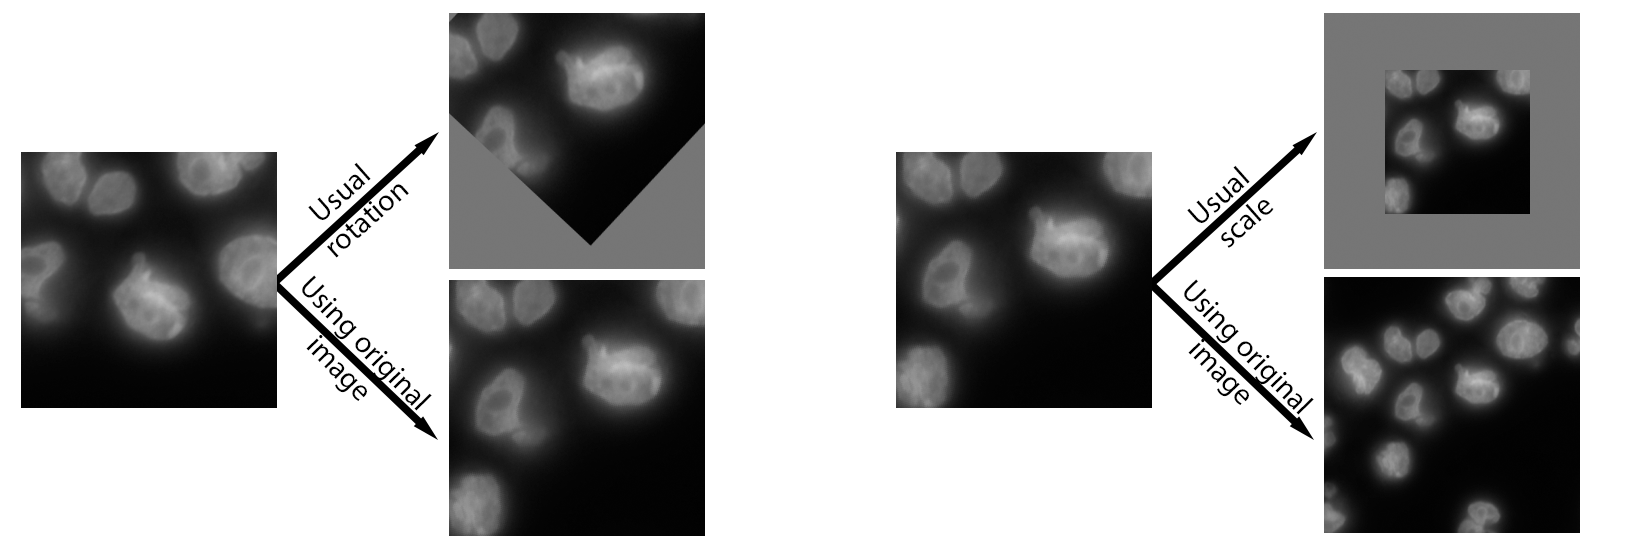
\includegraphics[width=0.7\linewidth]{bilder/model training/smart augmentations.png}
		\caption{Using original image for rotation and scaling augmentations}\label{fig:smart-augments}
	\end{center}
\end{figure}

Applying augmentations in combination with other regularization techniques has proven to be helpful against overfitting for the nuclei and ER training. Therefore it is recommended to use it in further research as well.

    \subsubsection{Model setup}
        \paragraph{Weight Initialization}
        In order to achieve best predictions results it is very important to pre-setup a model correctly. Since the architecture used here is very similar to the one used in LaChance paper, the setup configuration is similar as well.  
        Weight initialization plays a crucial role in model training. Even on the simplest model wrongly initialized weights (for example all constant or too large or too small) can lead to very slow convergence or prevent the model from converging at all (\cite{Kumar_2017}).

Xavier initialization, which is usually a default choice in many neural networks, works well for the most part for fully connected layers with tanh as activation function. There is also a study providing some insights into why Xavier initialization may not be the optimal choice for ReLU activations (\cite{Kumar_2017}). In the following samples \textit{fan\_in} denotes the maximum number of input signal units to a given layer and \textit{fan\_out} is the maximum number of output signal units from it. A definition of Xavier initialization can be found below:

Research of \cite{He_2015} also notices the problems with Xavier initialization for ReLU activations. The authors suggest a new robust method called He initialization that enables training of even extremely deep or wide network architectures with ReLU activations. This method was suggested by the \cite{Lachance_2020} paper and has been used in this reseach as well. He initialization draws samples from a truncated normal distribution:
\begin{equation}
	N(0, \sqrt{\frac{2}{\text{fan\_in}}})
\end{equation}

Default weight initialization of Conv2D layers in Python claims to uses the following initialization method the initialization method (\cite{He_2015}):
\begin{align}
	std &= \sqrt{\frac{2}{fan\_in}} \\
	bou&nd = \sqrt{3 * std} \\
	Un&iform(-bound, bound)
\end{align}

Altough in the study of \cite{He_2015} it is called Kaiming normal initialization it is not exactly it. However, the naming is quite confusing and therefore two experiments have been conducted: first, the model predicting nuclei target was trained with the default weight initialization provided by PyTorch and then the initialization was switched to a true He initialization.

\begin{figure}[H]
	\begin{center}
		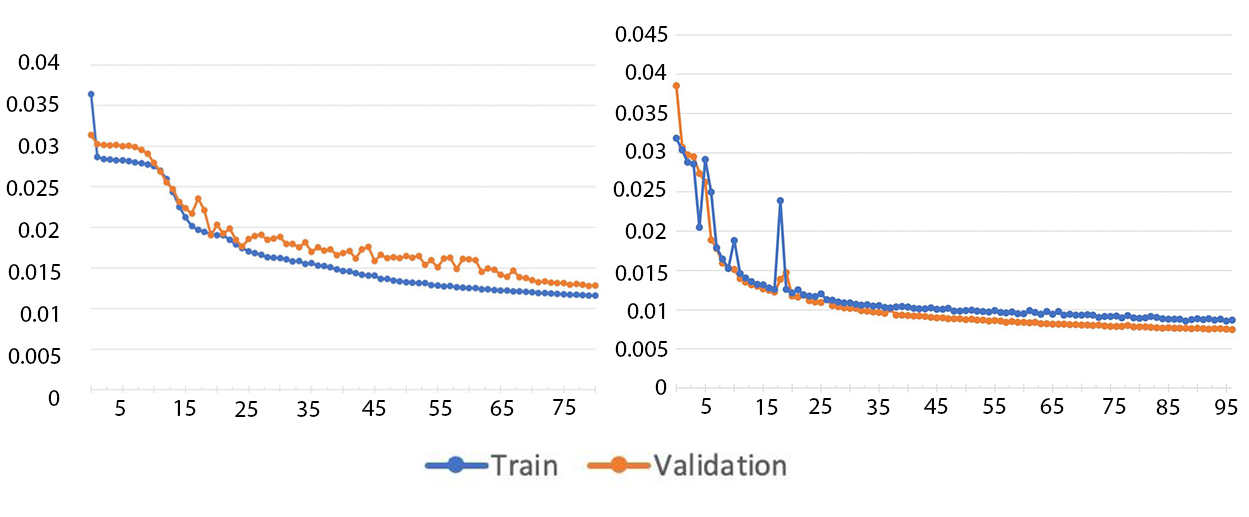
\includegraphics[width=0.8\linewidth]{bilder/nuclei/wi-no-wi.png}
		\caption[Nuclei training without (left) and with (right) custom weight initialization]%
		{Nuclei training without (left) and with (right) custom weight initialization. The stagnation during first few epochs on the left signalizes about the wrong initialization of model's weights. As a result the left model also converges to a higher value.}\label{fig:wi}
	\end{center}
\end{figure}

The results of the experiments are presented in Figure \ref{fig:wi}. As can be seen, the loss in the left plots stagnates during the first few epochs and then begins to converge later. This is a symptom of a wrong initialization of the weights. Even after the convergence begins, the model still has a higher loss than the one on the right (around 0.012 in comparison to 0.007). However, the model on the right is not completely perfect as the loss still does not converge at the same speed everywhere. Although this might be not related to the weight initialization but more the to instability of the training in general as there were only few images used for these experiments.

        \paragraph{Regularization}
        \label{section:regularization}
        % TODO add overfitting image?
Regularization is mostly used to prevent a deep learning model to overfitting on the training data and to be able to generalize well. Overfitting has occured in the models used in this research and therefore it is improtant to understand the techniques that can be used to prevent it. There are are several approaches to regularize the model and they will be explained below.

\begin{itemize}
	\item Early-stopping

	Overfitting can be detected via visualizing train and validation losses. Training behaviour at first will be the usual one, meaning that both train and validation losses are gradually decreasing, however at some point the train loss continues to decrease, whereas the validation loss suddenly starts to increase (see Figure \ref{fig:er-overfit}). Since the model has not seen any of the data from the validation set, it means that it loses its ability to generalize on unseen data, while improving its perfomance on the seen data (train set). This does not happen during earlier epochs. Assuming that the model learns a complex decision surface while training, the weights of the model will be quite small and random with the correct weight initialization and therefore the best decision surface during the early epochs would be a smooth one. But during the later ones the difference in values of the weights grows and they become dissimilar which also means that the decision surface becomes more complex and the model is now able to fit not only the training data itself, but also its noise (\cite{mitchell_1997} p.111). And that is why stopping before the model becomes too complex, meaning to stop before the overfitting point, mitigates this problem.

	\item \emph{L1}- \emph{L2}-regularization

	The complexity of the deep model grows with the number of features it uses, sometimes the model may pay attention to the features that are not important to the outcome, or even considers noise to be a feature. To prevent this one should decrease the weights associated with useless features, however one cannot know ahead of time which of them should be ignored, therefore one may limit them all (\cite{Ying_2019}). In order to do that, a penalty term is added to the loss function:

	\begin{equation}
	\tilde{L}(Y, M(X, \theta)) = L(Y, M(X, \theta)) + \lambda R(\theta)
	\end{equation}

	for some $\lambda > 0$. This is called a \emph{soft-constraint} optimization. When $R(\theta)$ is of the form $R(\theta) = ||\theta||^2_2 = \sqrt{\sum\limits_i \theta_i^2}$ this is called \emph{L2}-regularization. When it is of form $R(\theta) = ||\theta||_1 = \sum\limits_i |\theta_i|$ this is called \emph{L1}-regularization. \emph{L2}-regularization used in combination with backpropagation is equivalent to weight decay. Weight decay is defined by \cite{Hanson_1988} as follows:
	\begin{equation}
		\theta_{t+1} = (1 - \lambda)\theta_t - \alpha \frac{\partial L}{\partial \theta_t}
	\end{equation}

	where $\alpha$ is a learning rate. Weight decay successfully has more effect on the weights along which the gradient change is smaller \cite{Goodfellow_2016}. \emph{L1}-regularization induces sparsity of the weights by assigning some of them to zero, this could also be considered as a feature selection approach.

	\item Regularization layers

	Batch normalization and dropout layers are also considered to be a form of regularization.

	\item Network reduction

	Since learning a too complex and noise-fitting decision surface might be a frequent cause of an overfit, another way to mitigate this would to be reduce the space of the possible decision surfaces and therefore make the surface simpler so that it cannot fit into the noise from the data. By changing the number of adaptive parameters in the network, the complexity can be varied (\cite{Bishop_2006} p.332).

	\item Expansion of the training data

	For a successful training a model needs to have a sufficient amount of quality samples. An expanded dataset can improve the quality of the predictions \cite{Ying_2019}, however only when the model has already performed well on the initial dataset. If the model was performing badly initially, adding more data will not solve the problem. Here having $27,264$ crops of data the model was trained on $5,376$ crops only (two 96-well plates) to find the best structure and regularization first, afterwards the model was retrained using more data and the PCC loss improves from $0.77$, to $0.93$.
\end{itemize}

        \paragraph{Optimizers}
        It is also important to choose a correct optimizer in order for a model to converge as fast as possible. Here, three different optimizers have been tried out --- namely, SGD, Adam and Adadelta optimizers. As a result, the SGD optimizer performed the worst, while Adam and Adadelta optimizer performed similarly with Adadelta converging to slightly better values in the end. Adam optimizer has required some fine-tuning of the learning rate from 0.001 to 0.0001 to achieve the best result. Both Adadelta and Adam can be used for model optimization in this dataset. The experiments were conducted on the truncated dataset of nuclei images using PCC loss.

\begin{figure}[H]
	\begin{center}
		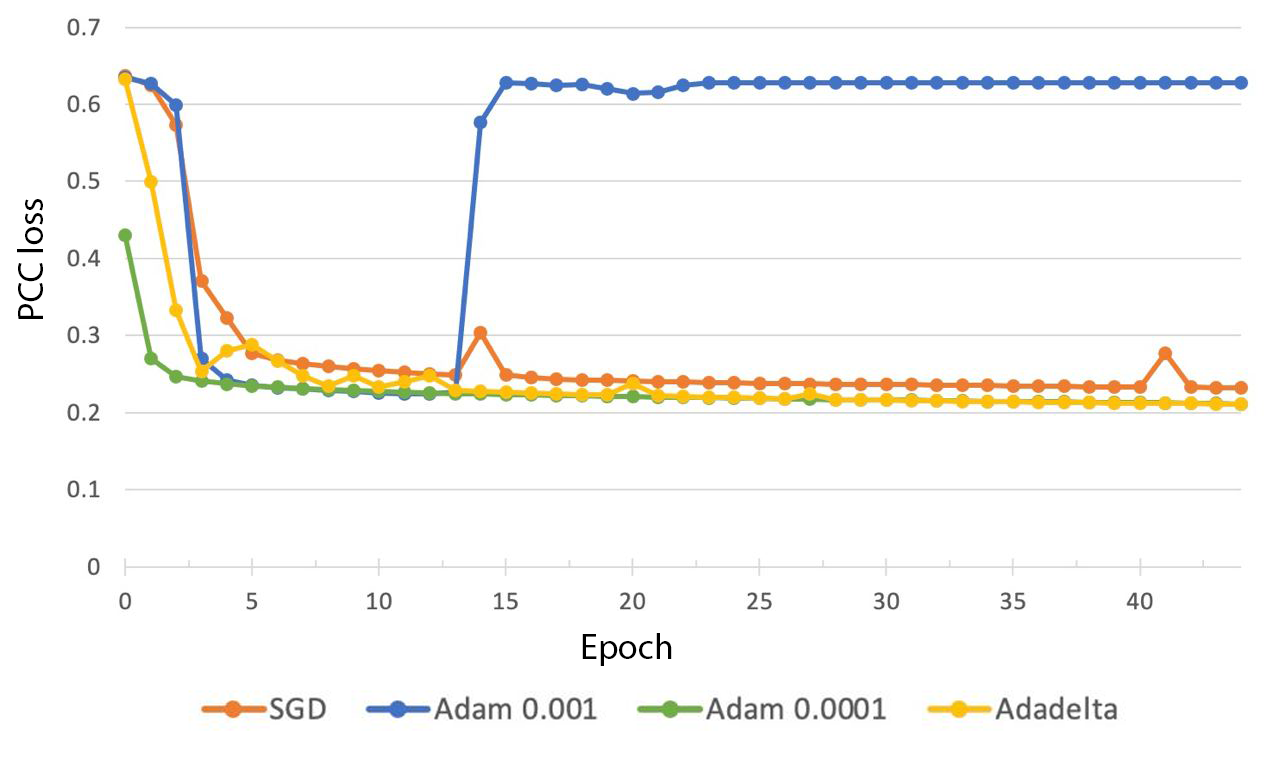
\includegraphics[width=0.8\linewidth]{bilder/model training/optimizer-comparison.png}
		\caption{Comparison of convergence for different optimizers}\label{fig:optimizers}
	\end{center}
\end{figure}


    \pagebreak
    \subsection{Nuclei}
    A nucleus (plural nuclei), as related to genomics, is the membrane-enclosed organelle within a cell that contains the chromosomes. The nucleus is one of the easiest organelle to detect within the cell as it is usually located in the middle and occupies quite a big area of the cell (see Figure \ref{fig:cell}). Nucleus contains all of the cell's chromosomes, which in their turn encode the genetic material, therefore nucleus is a very important organelle (\cite{genomegov}). In order to stain it, DAPI was added to the cells. This is a fluorescent stain that binds strongly with some regions in DNA. Analysis of cell's nucleus can provide many valuable insights, for example the radius of living cells is on average bigger then in dead ones (\cite{Christiansen_2018}). With fluorescence labeling one can derive some useful features used for determining whether the well plate should or should not be selected during the selection step in CLD process.
    %cite Christiansen 2018]  proves only success on nuclei for DIC
    \begin{figure}[htb]
        \begin{center}
            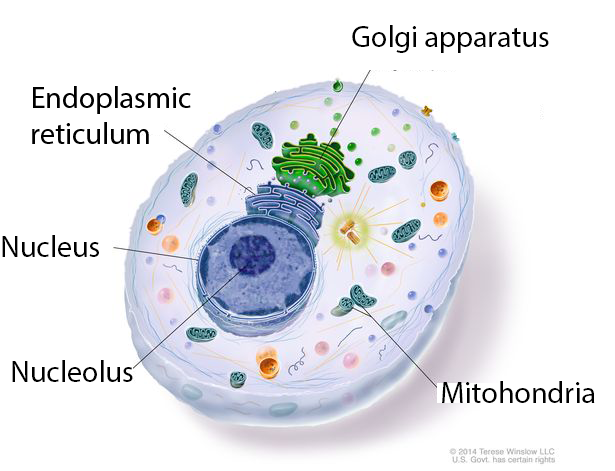
\includegraphics[width=0.3\linewidth]{bilder/cell structure.png}
            \caption{Cell structure}\label{fig:cell}
        \end{center}
    \end{figure}

    \subsubsection{Preprocessing}\label{section:nuclei-preprocessing}
        As not all of the dataset samples were of the same quality it was important to first manually filter the dataset to remove the bad imaging samples. Even with the normal conditions many of the images contain a lot of background. This creates a background vs. foreground class imbalance (see Figure \ref{fig:bad-smaples}a). Overexposure is also a typical problem that creates samples of a too high intensity and with details inside the nucleus missing (see Figure \ref{fig:bad-smaples}b, c). Lastly, underexposure is just as problematic as overexposure (see Figure \ref{fig:bad-smaples}d).

\begin{figure}[H]
	\begin{center}
		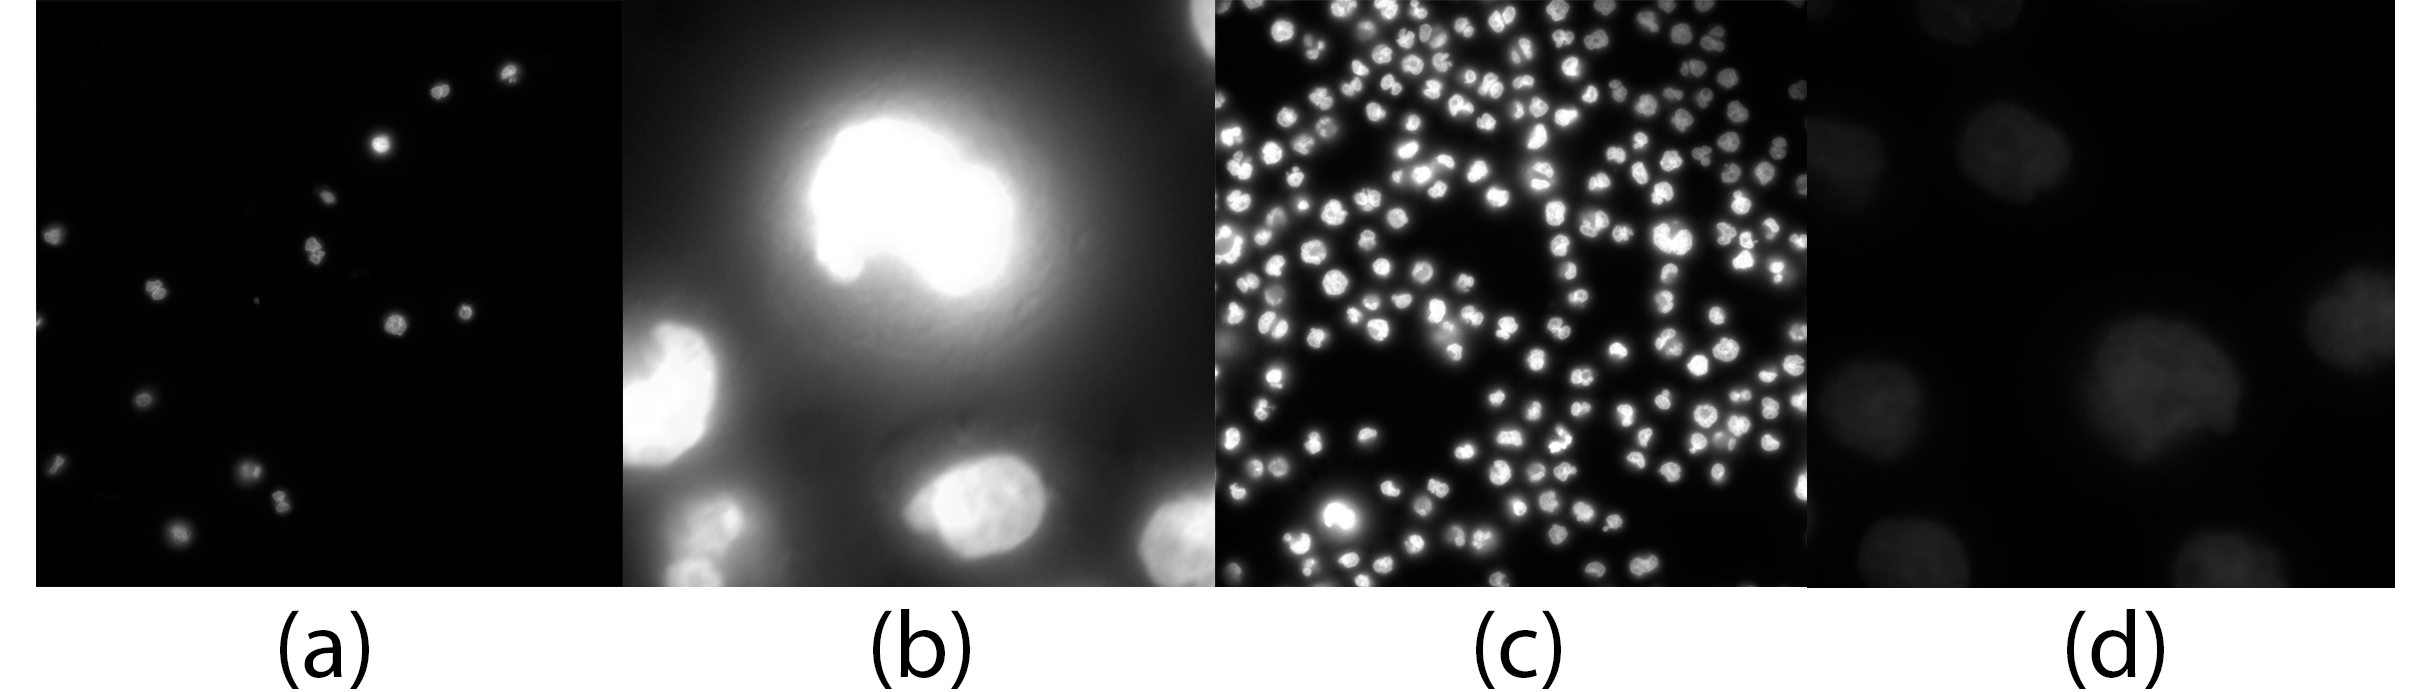
\includegraphics[width=0.7\linewidth]{bilder/nuclei/filter-out.png}
		\caption[Nuclei fluorescence samples to be filtered out]%
		{Nuclei fluorescence samples to be filtered out. (a) --- too few cells in the image result in many fully black crops; (b) --- overexposure; (c) --- overexposure, lack of details; (d) --- underexposure.}\label{fig:bad-smaples}
	\end{center}
\end{figure}

Once the images have been filtered out, they were normalized to have the values between 0 and 1.

    \subsubsection{Training and predictions}
        \paragraph{Convergence}
              %\begin{figure}[H]
%	\begin{center}
%		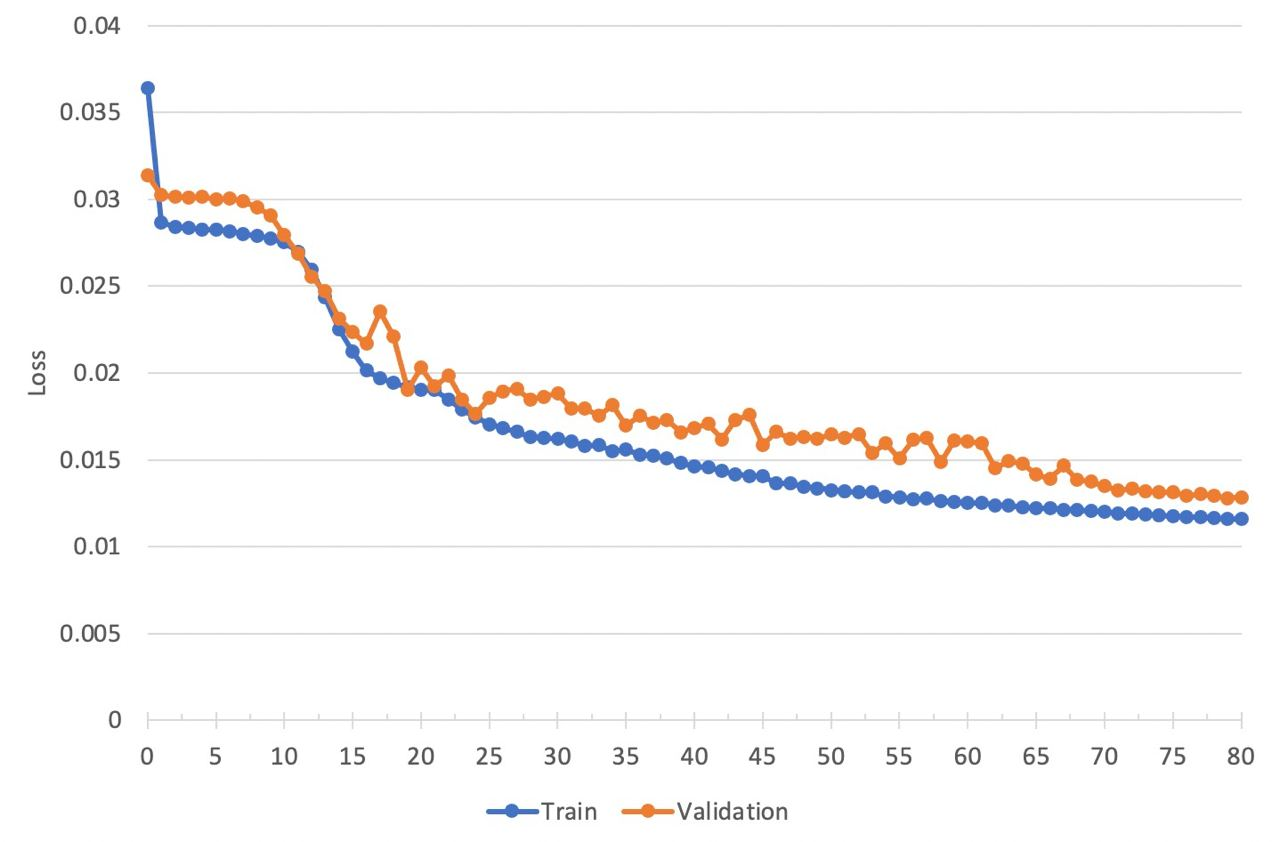
\includegraphics[width=0.5\linewidth]{bilder/nuclei/no-wi.jpg}
%		\caption{Default weight initialization is not suitable}\label{fig:no-wi}
%	\end{center}
%\end{figure}

%\begin{figure}[H]
%	\begin{center}
%		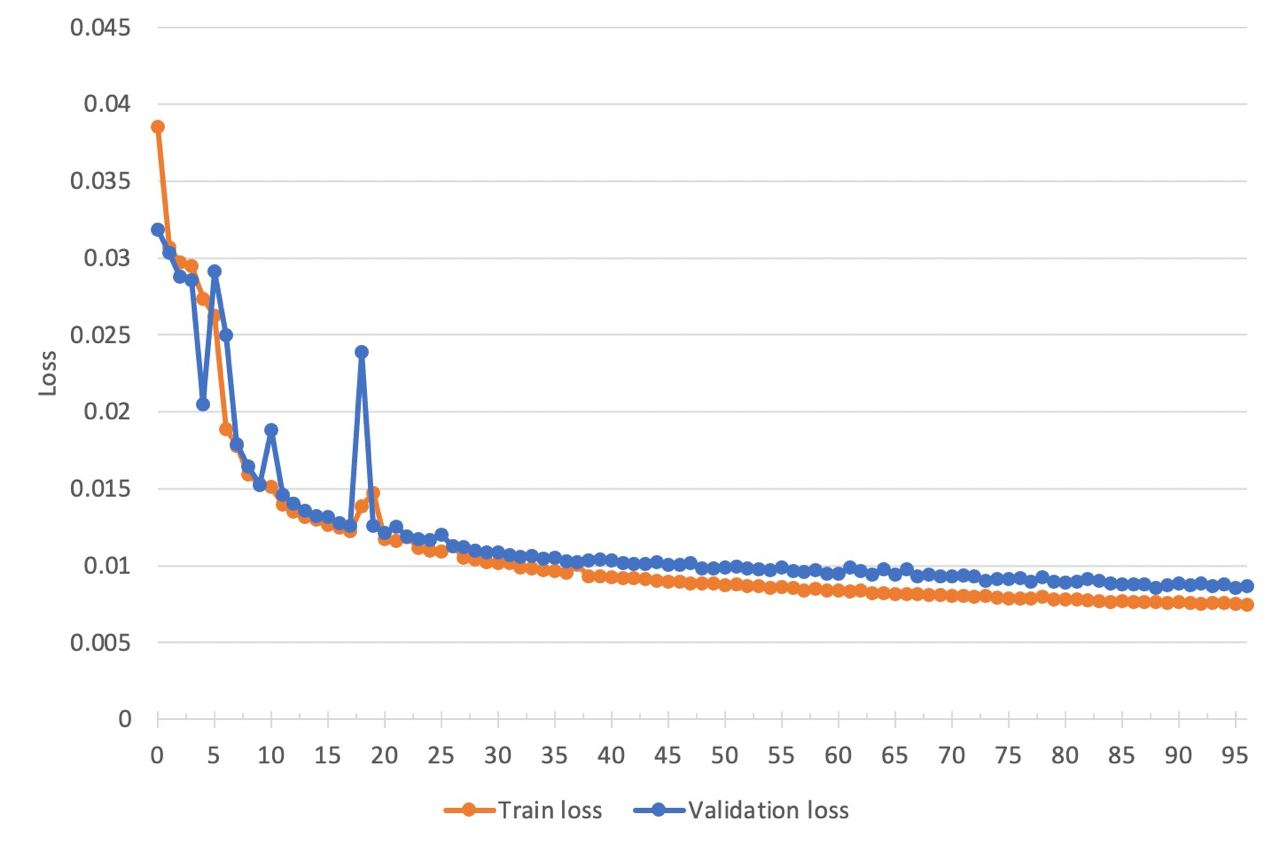
\includegraphics[width=0.5\linewidth]{bilder/nuclei/pca-2-datasets.jpg}
%		\caption{PCC with correct weight initialization converges but unstable}\label{fig:pcc-2-dataset}
%	\end{center}
%\end{figure}

As the nuclei dataset is one of the biggest ones (see Table \ref{table:data}), the experiments would first be performed on the subset of the data, and only once the training pipeline and good results were established, the training would be done using the full dataset. Figure \ref{fig:wi} (right) represents the training of nuclei using only two 96-well plates with MSE loss. The training is very unstable in the begining, but one can clearly see that the model successfully converges afterwards. Our hypothesis behind the instability was the clear lack of training data, which was proven by further training using the full data and as a result achieving a more stable PCC loss (see Figure \ref{fig:full-dataset-pcc}).

\begin{figure}[htb]
	\begin{center}
		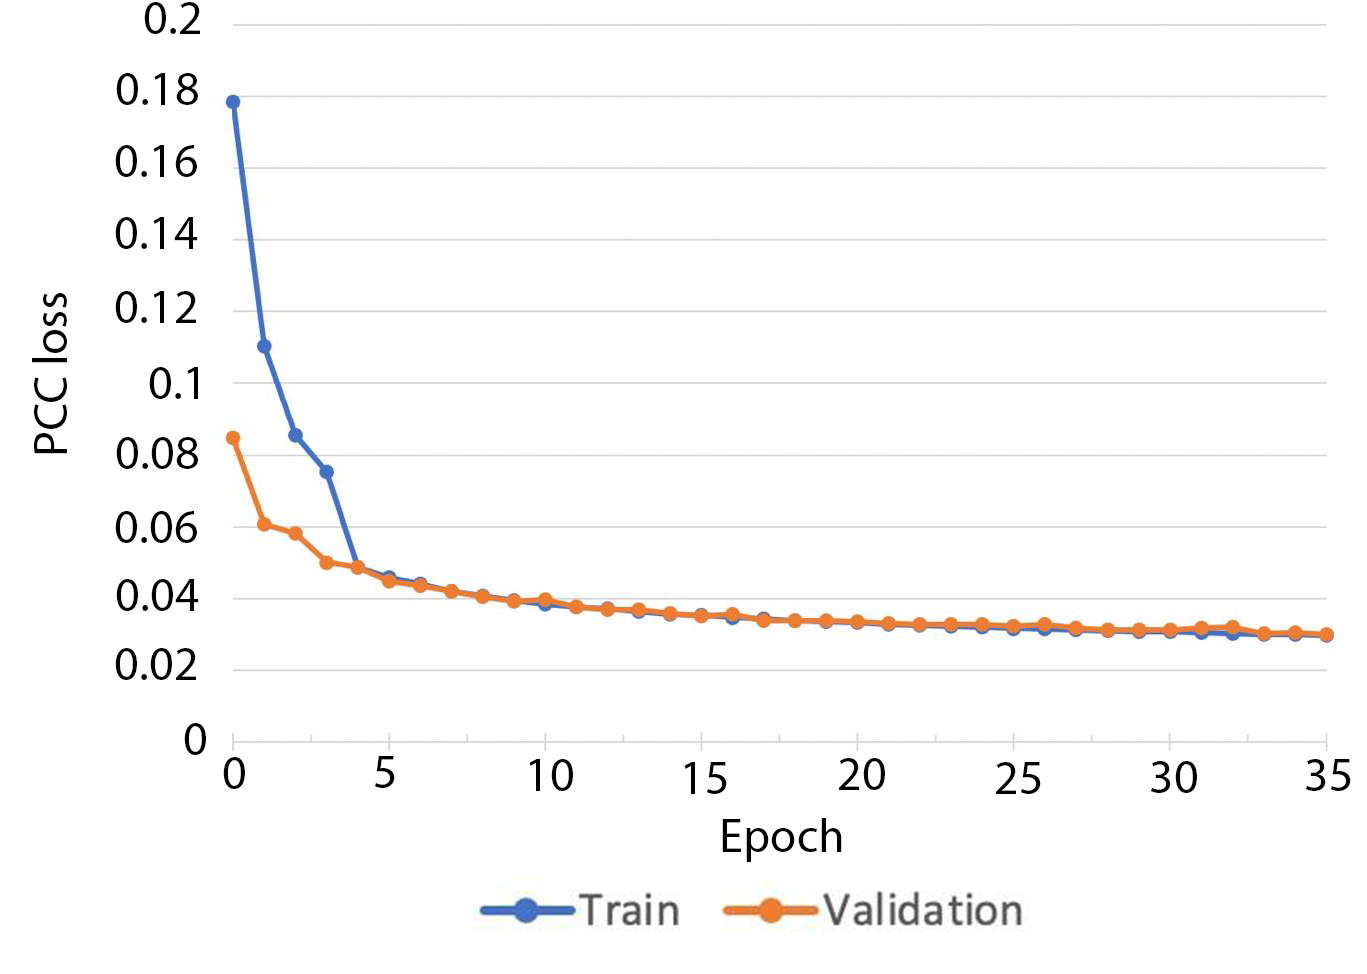
\includegraphics[width=0.5\linewidth]{bilder/nuclei/full-dataset.png}
		\caption{Having more data makes training more stable}\label{fig:full-dataset-pcc}
	\end{center}
\end{figure}

As mentioned in definition \ref{def:pcc-loss} for correct understanding of the following plots, one should be careful with differentiating PCC loss from PCC itself. PCC loss converts PCC to be between $0$ and $1$, with $0$ being an optimal value.

Seeing that the model significantly stabilizes with the use of more data and that the prediction results become much more similar to the ground truth (see Figure \ref{fig:nuclei-comparison-predictions} \textit{small dataset} vs. \textit{full dataset}), it was decided to try the use of augmentations in order to enlarge the dataset even more. In this case the augmentations were not used in order to regularize or stabilize training (by providing more difficult, for instance, blurred samples), but to simply have more data. Training and validation PCC losses from the training with the use of augmented data are presented in Figure \ref{fig:no-reg-augmented}. The augmentations used here are horizontal and vertical flips, rotations and crops (described in detail in section \ref{section:augmentations}).
\begin{figure}[H]
	\begin{center}
		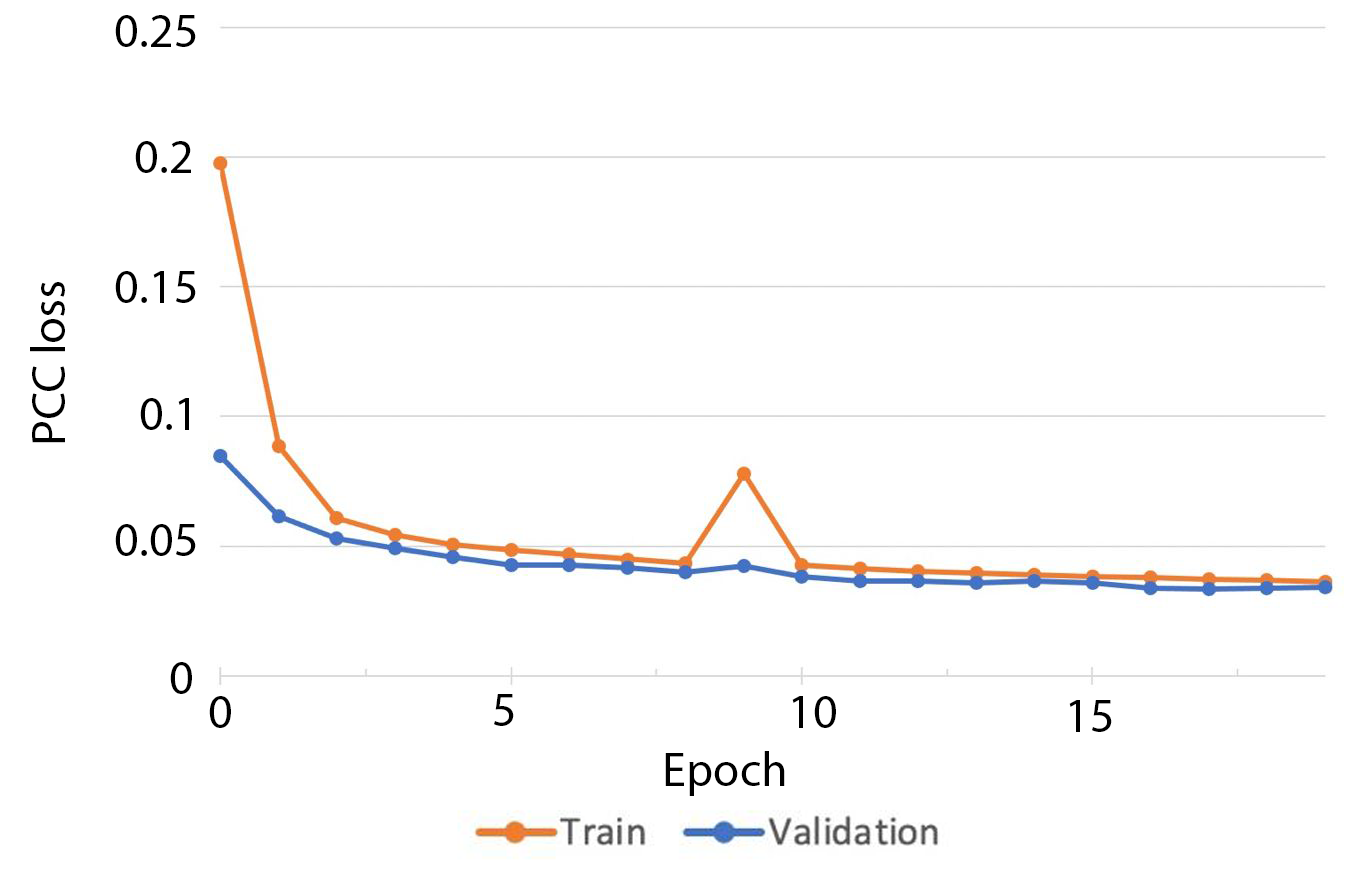
\includegraphics[width=0.5\linewidth]{bilder/nuclei/no-reg-but-aug.png}
		\caption{Adding simple augmentations in the dataset}\label{fig:no-reg-augmented}
	\end{center}
\end{figure}
Validation PCC loss has slightly increased to $0.0381$ in comparison to the previous value of $0.0365$. However, the validation set on which this loss was estimated also includes augmentations mentioned above and therefore presents a slightly more difficult task than the original validation set. True improvement is confirmed by measuring the loss of the models on the same dataset, where PCC loss has improved from $0.0365$ to $0.0322$ (or PCC from $0.92$ to $0.93$).

In the next experiment the model has additionally been regularized by adding dropout layers and using a weight decay of $0.0001$ (see Figure \ref{fig:full-dataset-pcc-regularized}). This did not bring a better result, but has only made it more difficult for the model to capture the needed feature to reproduce the fine details within the nuclei. However, this brought up a new hypothesis, namely that the model might simply have not enough of capacity to capture enough of the details. In order to confirm this a bigger model has to be trained.
\begin{figure}[htb]
	\begin{center}
		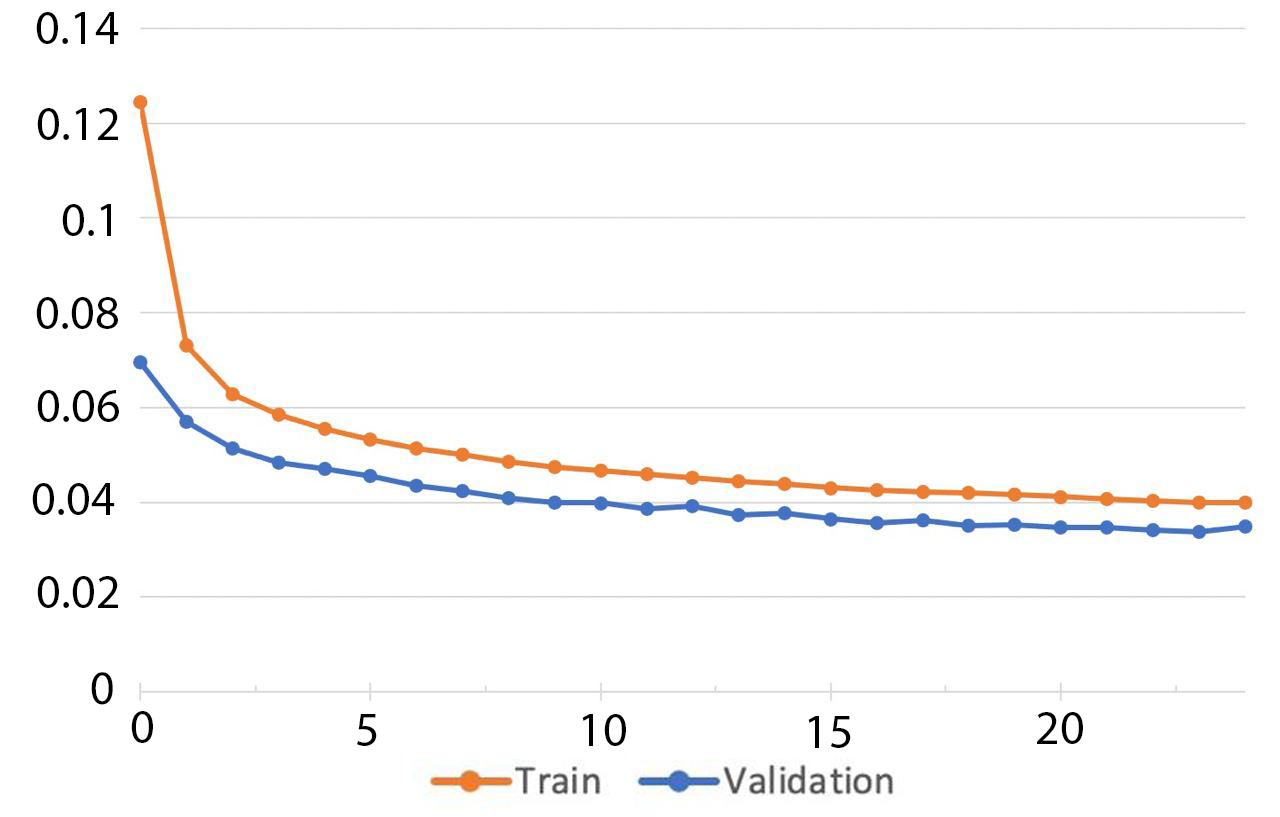
\includegraphics[width=0.5\linewidth]{bilder/nuclei/full-dataset-regularized.png}
		\caption{With regularization and augmentations}\label{fig:full-dataset-pcc-regularized}
	\end{center}
\end{figure}

\begin{figure}[htb]
	\begin{center}
		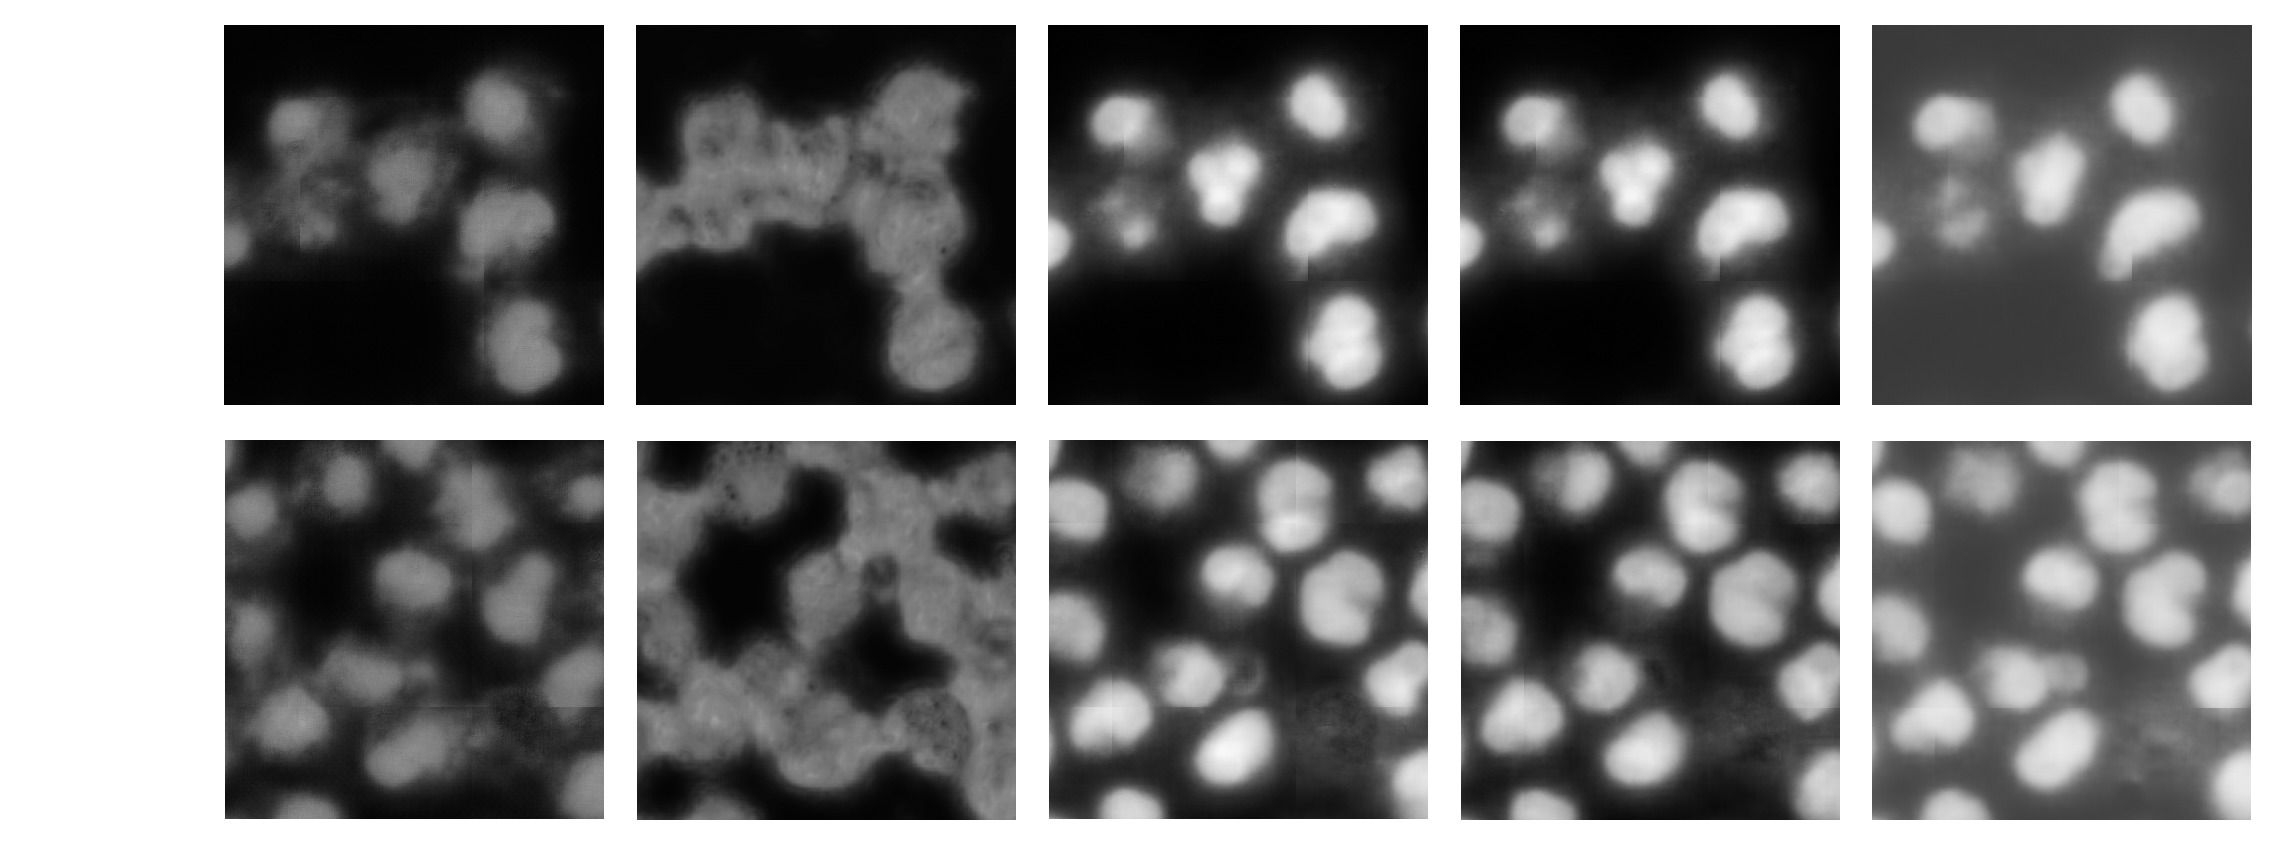
\includegraphics[width=0.6\linewidth]{bilder/nuclei/comparison-chzn-phx.png}
		\caption[Comparison of different models predictions and scores]%
		{Comparison of different models predictions and scores. PCC loss is representative of predictions quality, whereas MSE loss is not. Increasing model's size significantly improves the results.}\label{fig:nuclei-comparison-predictions}
	\end{center}
\end{figure}

Interestigly observations made in this section made it clear that metrics used for training (PCC and MSE losses) are indeed not representative enough to derive any conclusions regarding the model quality from them. Just by looking at Figure \ref{fig:nuclei-comparison-predictions} one can see that for example, training on the full dataset of data gives much better results than training on the small dataset. Yet MSE seems to be bigger for this experiment. Also, it is not representative in comparison of a model without the correct weight initialization vs. the regularized model with augmentations. MSE loss is much higher there, because in general the image became somewhat brighter, even though the quality of the nuclei is significantly better. PCC loss seems to represent the desired quality of the model better. This trend has been noticed by \cite{Lachance_2020} as well. They state that values of PCC lack the practical context --- which value would be good enough and good enough in which context? This issue has been addressed here as well in section \ref{section:model-evaluation}, where more practical metrics are introduced and the model evaluation on them is carried out.

        \paragraph{Predictions quality}
              \begin{figure}[H]
	\begin{center}
		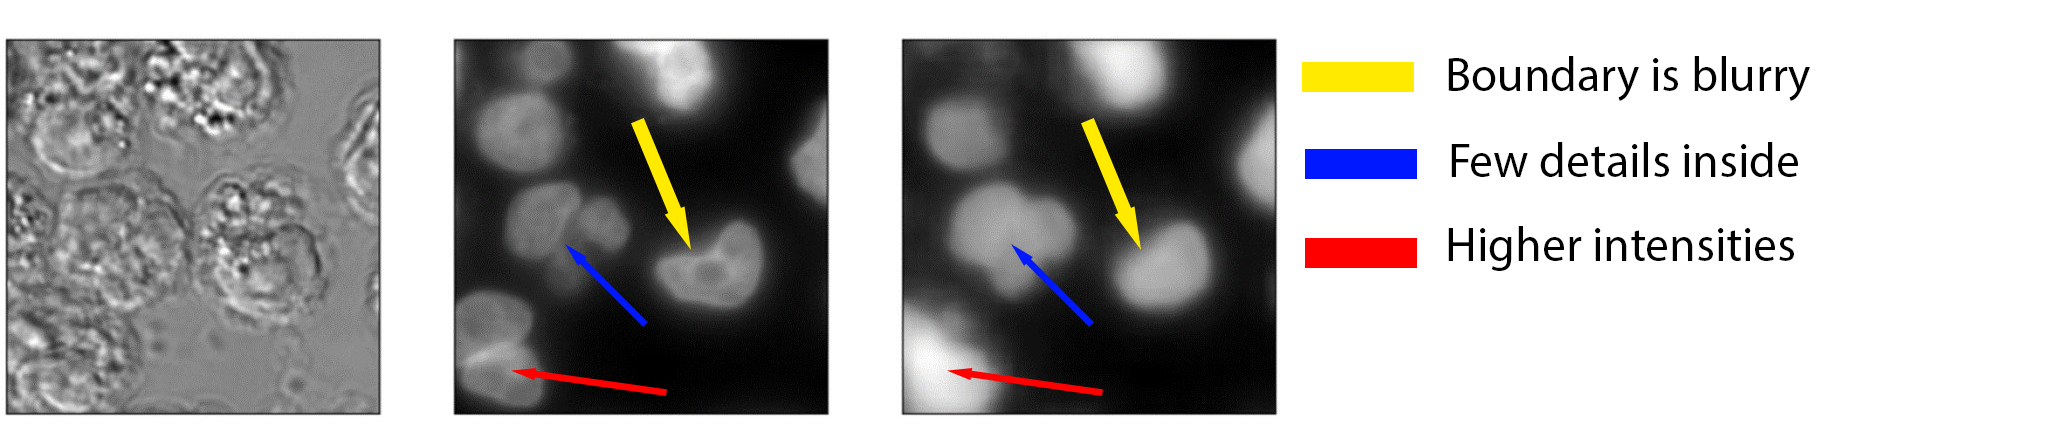
\includegraphics[width=0.8\linewidth]{bilder/nuclei/problems.png}
		\caption{Problems in predictions}\label{fig:nuclei-troubles}
	\end{center}
\end{figure}

\begin{figure}[H]
	\begin{center}
		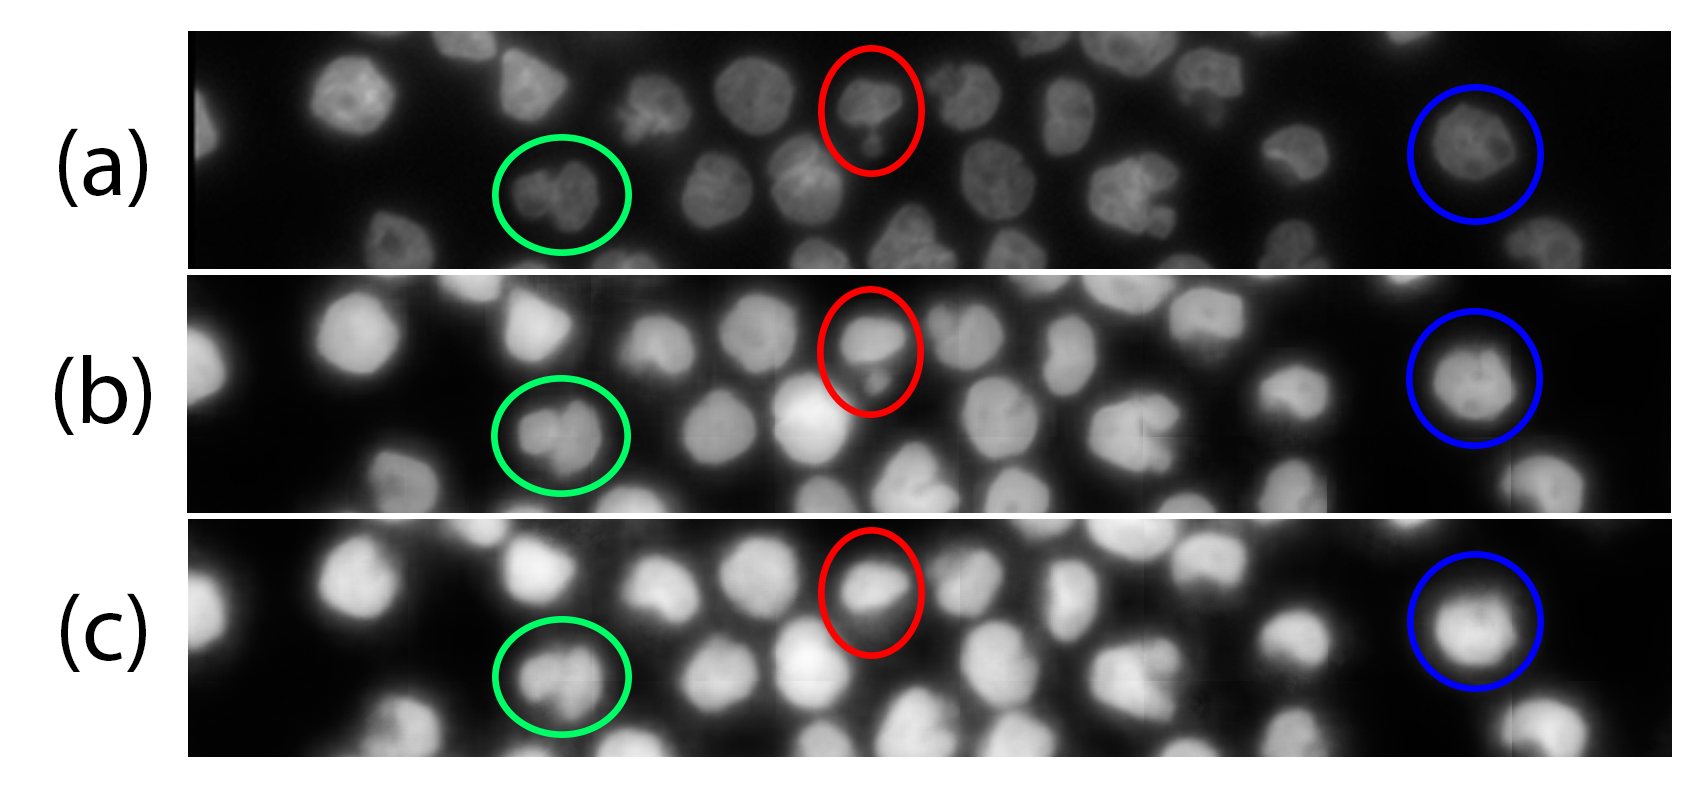
\includegraphics[width=0.6\linewidth]{bilder/nuclei/bigger-model.png}
		\caption{Predictions improvement}\label{fig:better-nuclei}
	\end{center}
\end{figure}
    \subsubsection{Postprocessing for nuclei segmentation}
        To properly evaluate the practical biological metrics described in section \ref{section:model-evaluation} on model predictions, one must be able to segment nuclei from fluorescence (as well as from predictions) first. Segmentation in this context refers to the creation of a mask. It should consist of $0$s and $1$s,  with a one being assigned to every pixel that is a part of the nucleus, while all the other ones are assigned with a zero. Although this might be a straightforward task for our eyes, it is not that easy to select separate nuclei via postprocessing. There are several edge cases where the nuclei are difficult to segment.

Even though the most extreme corruptions mentioned in section \ref{section:nuclei-preprocessing} were filtered out, some of the images that are corrupted not as severely (meaning they still have all the visible features needed for learning) are still present in the dataset, hence avoiding significant reduction of the amount of data.
\begin{figure}[H]
    \centering
    \setkeys{Gin}{width=\linewidth}
    \centering
        \begin{tabularx}{\textwidth}{YYYY}
            \textbf{Too few cells} &
            \textbf{Overexposure} &
            \textbf{Light gradient} &
            \textbf{Normal lighting} \\
            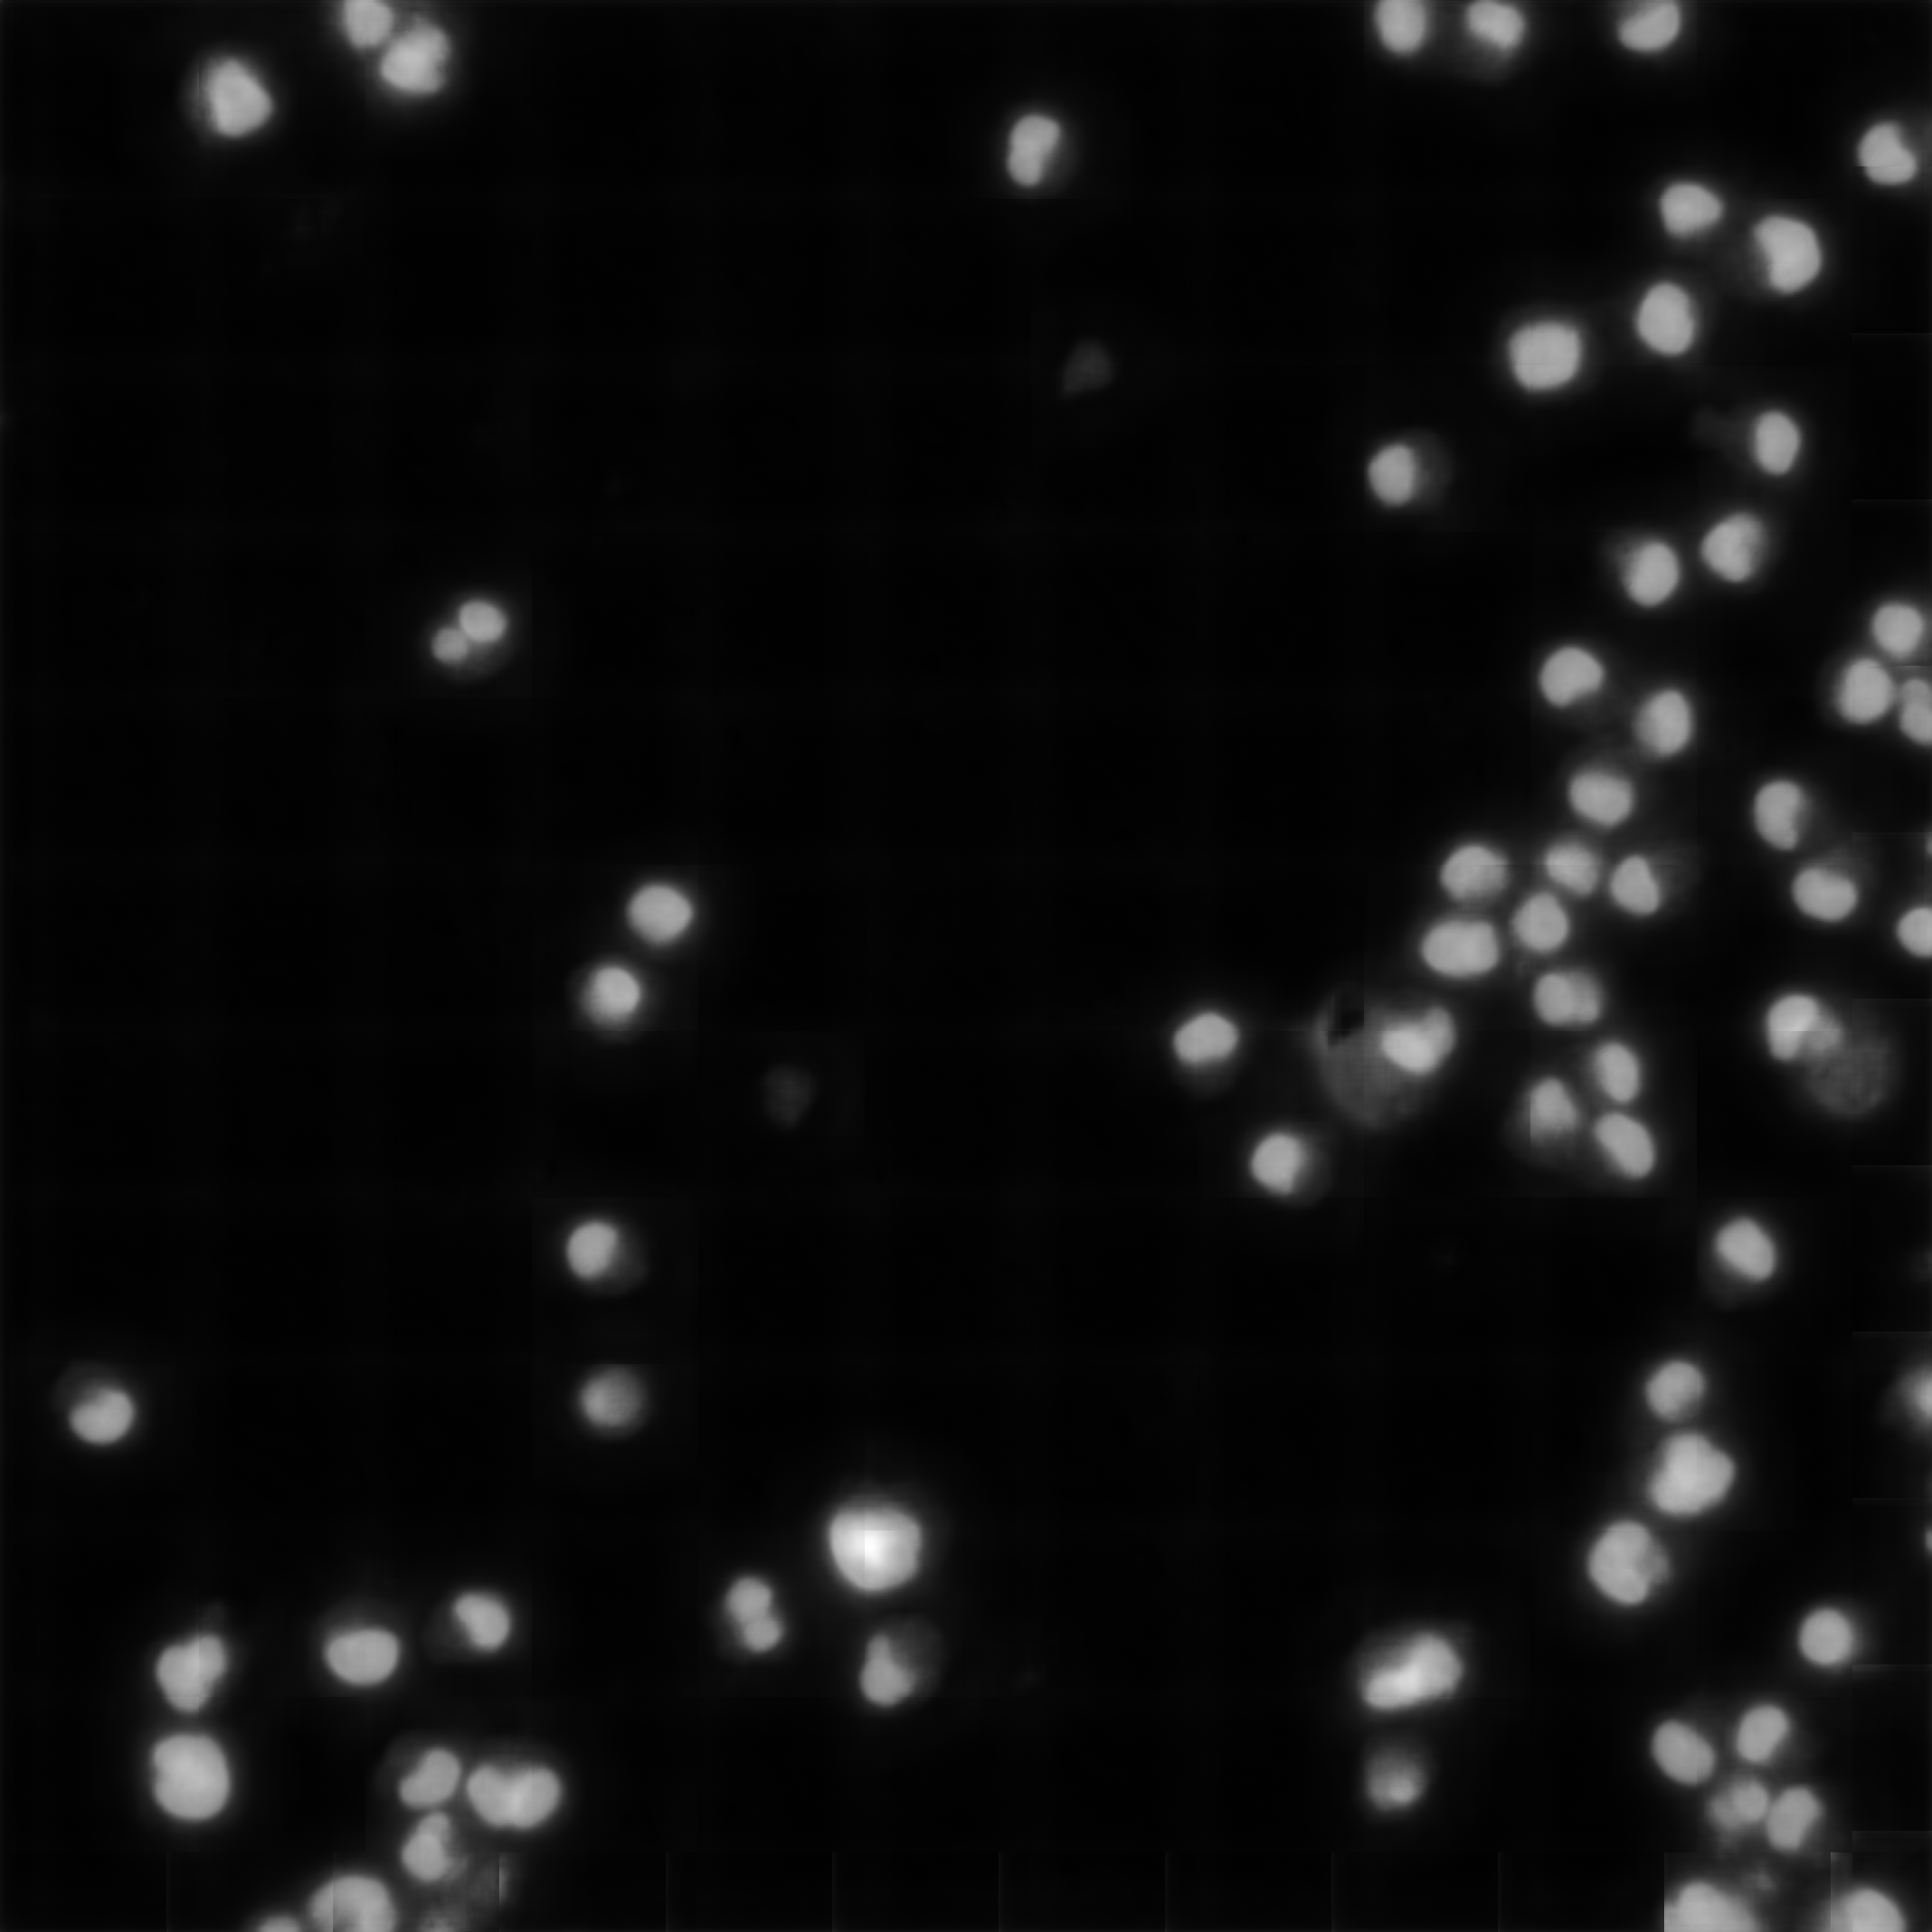
\includegraphics{bilder/lightning-conditions/lightning-1.png} & 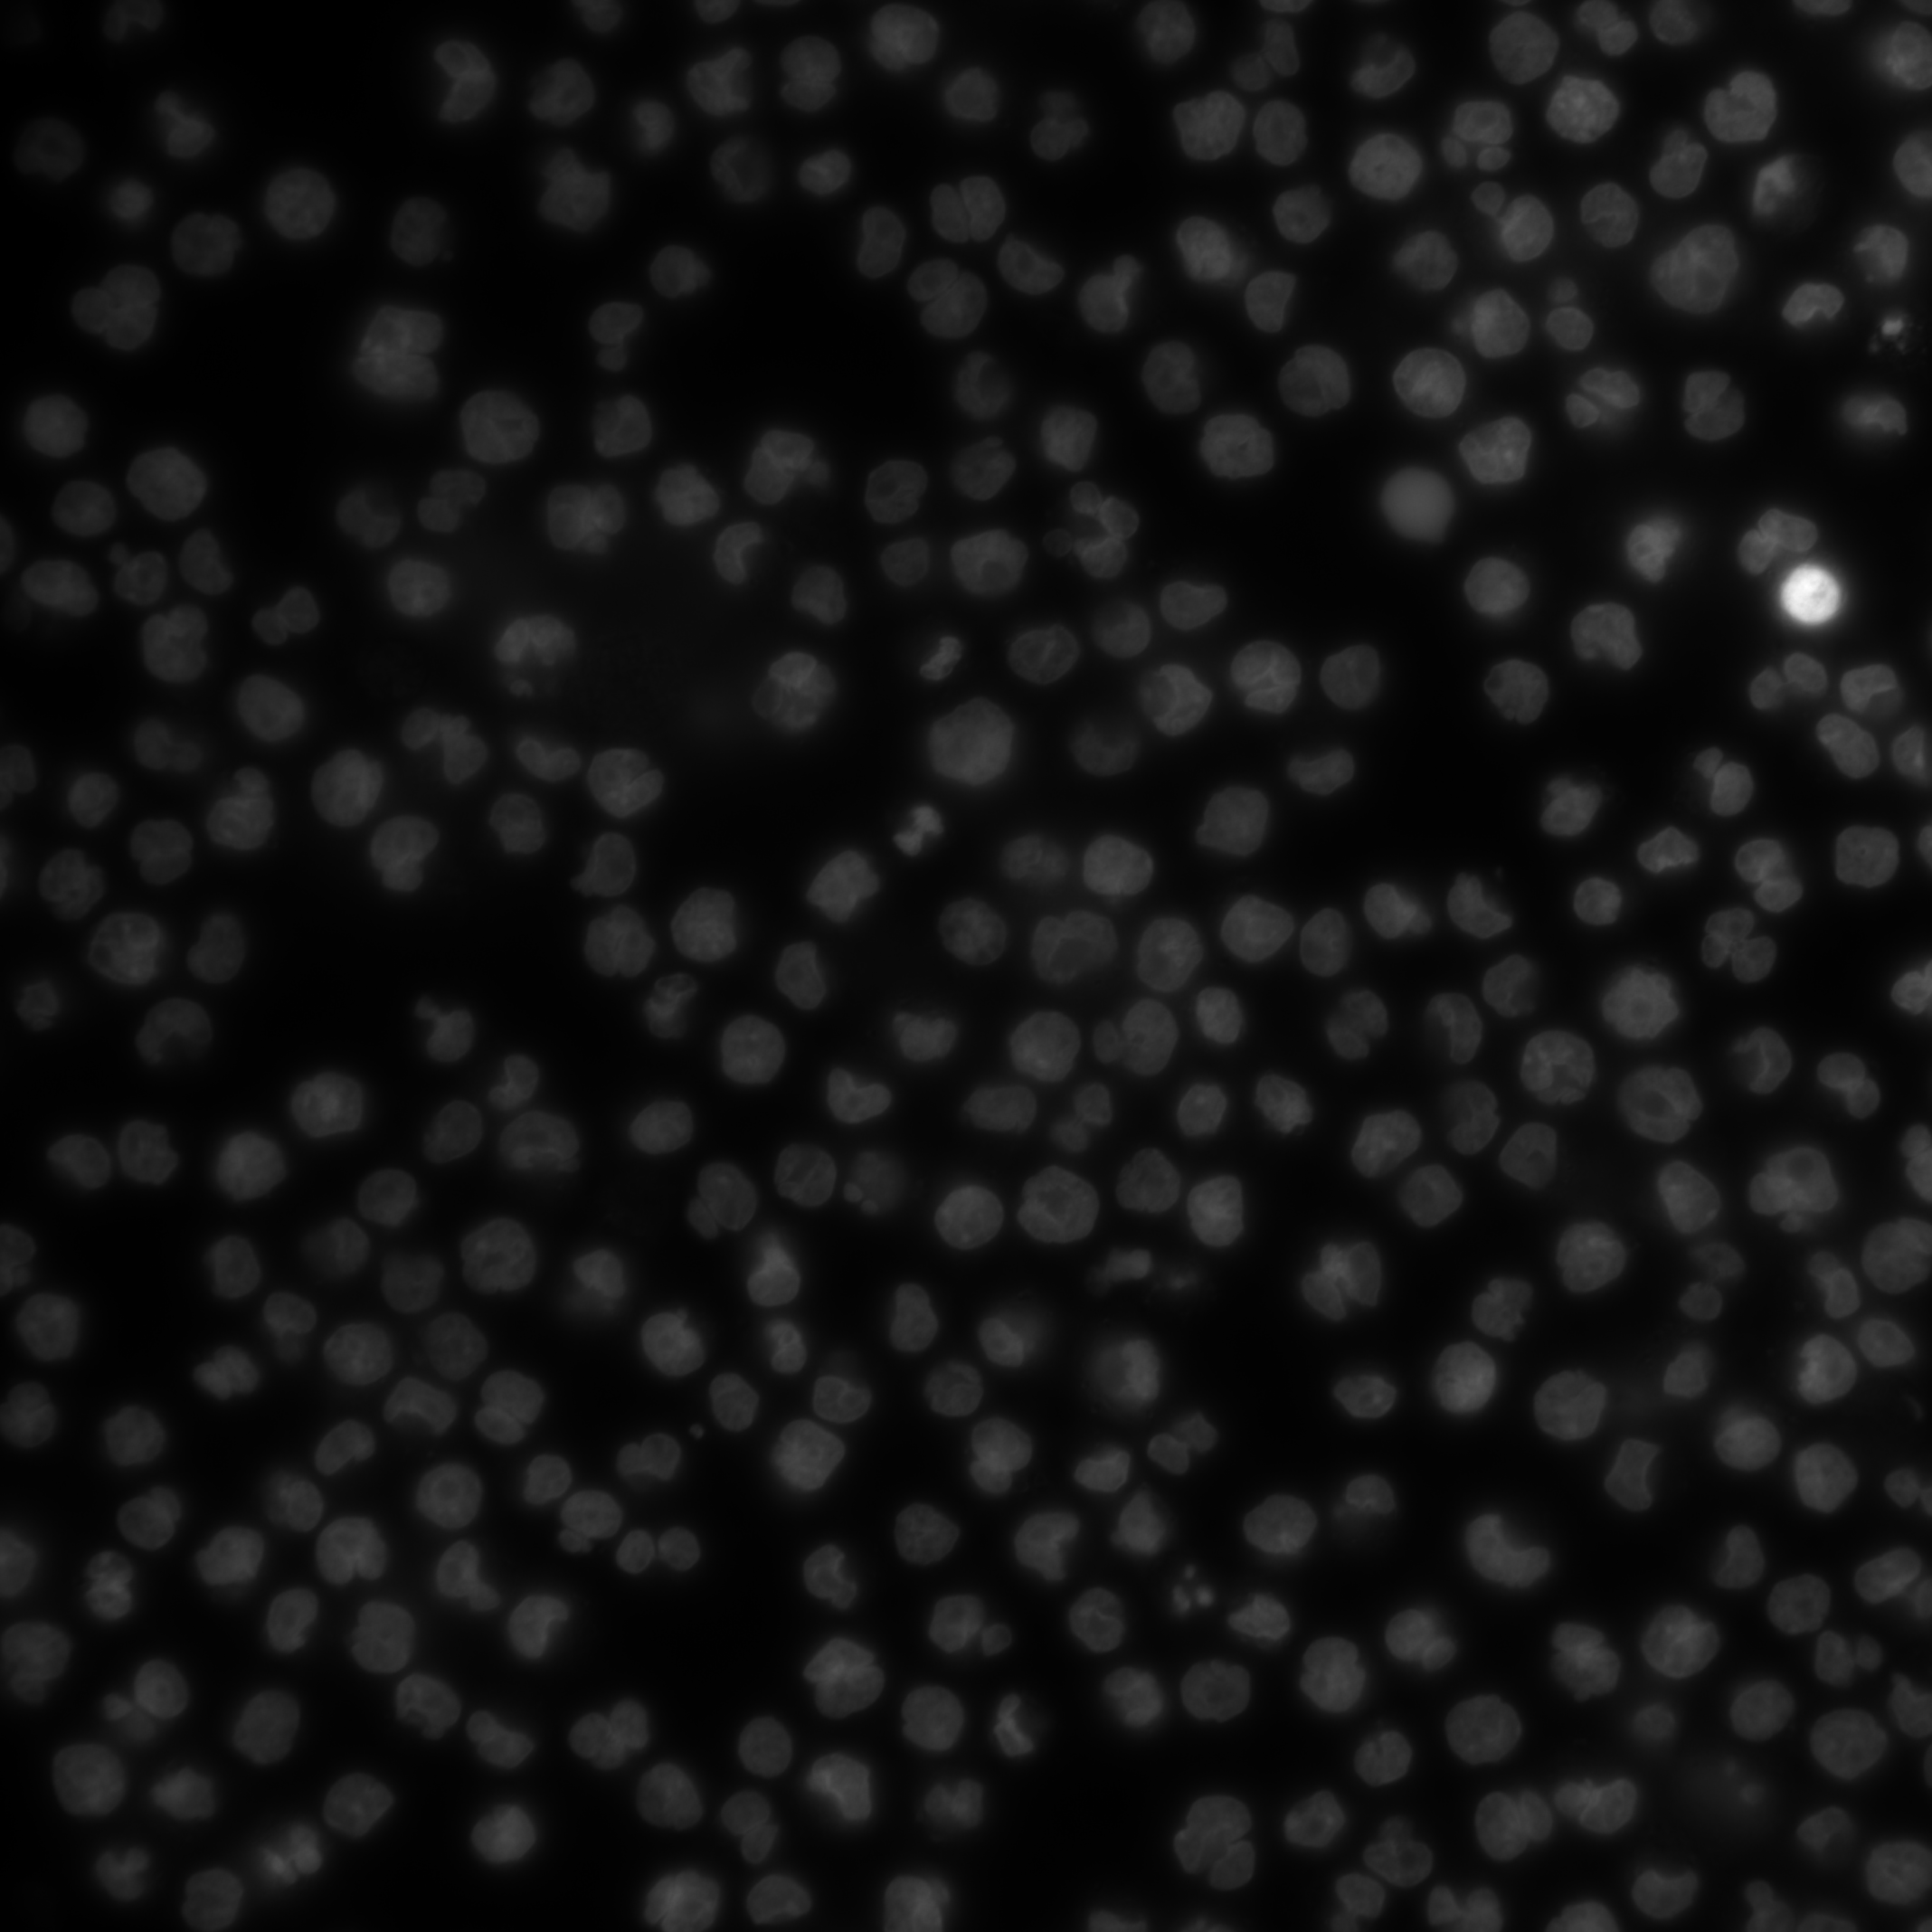
\includegraphics{bilder/lightning-conditions/lightning-2.png} &
            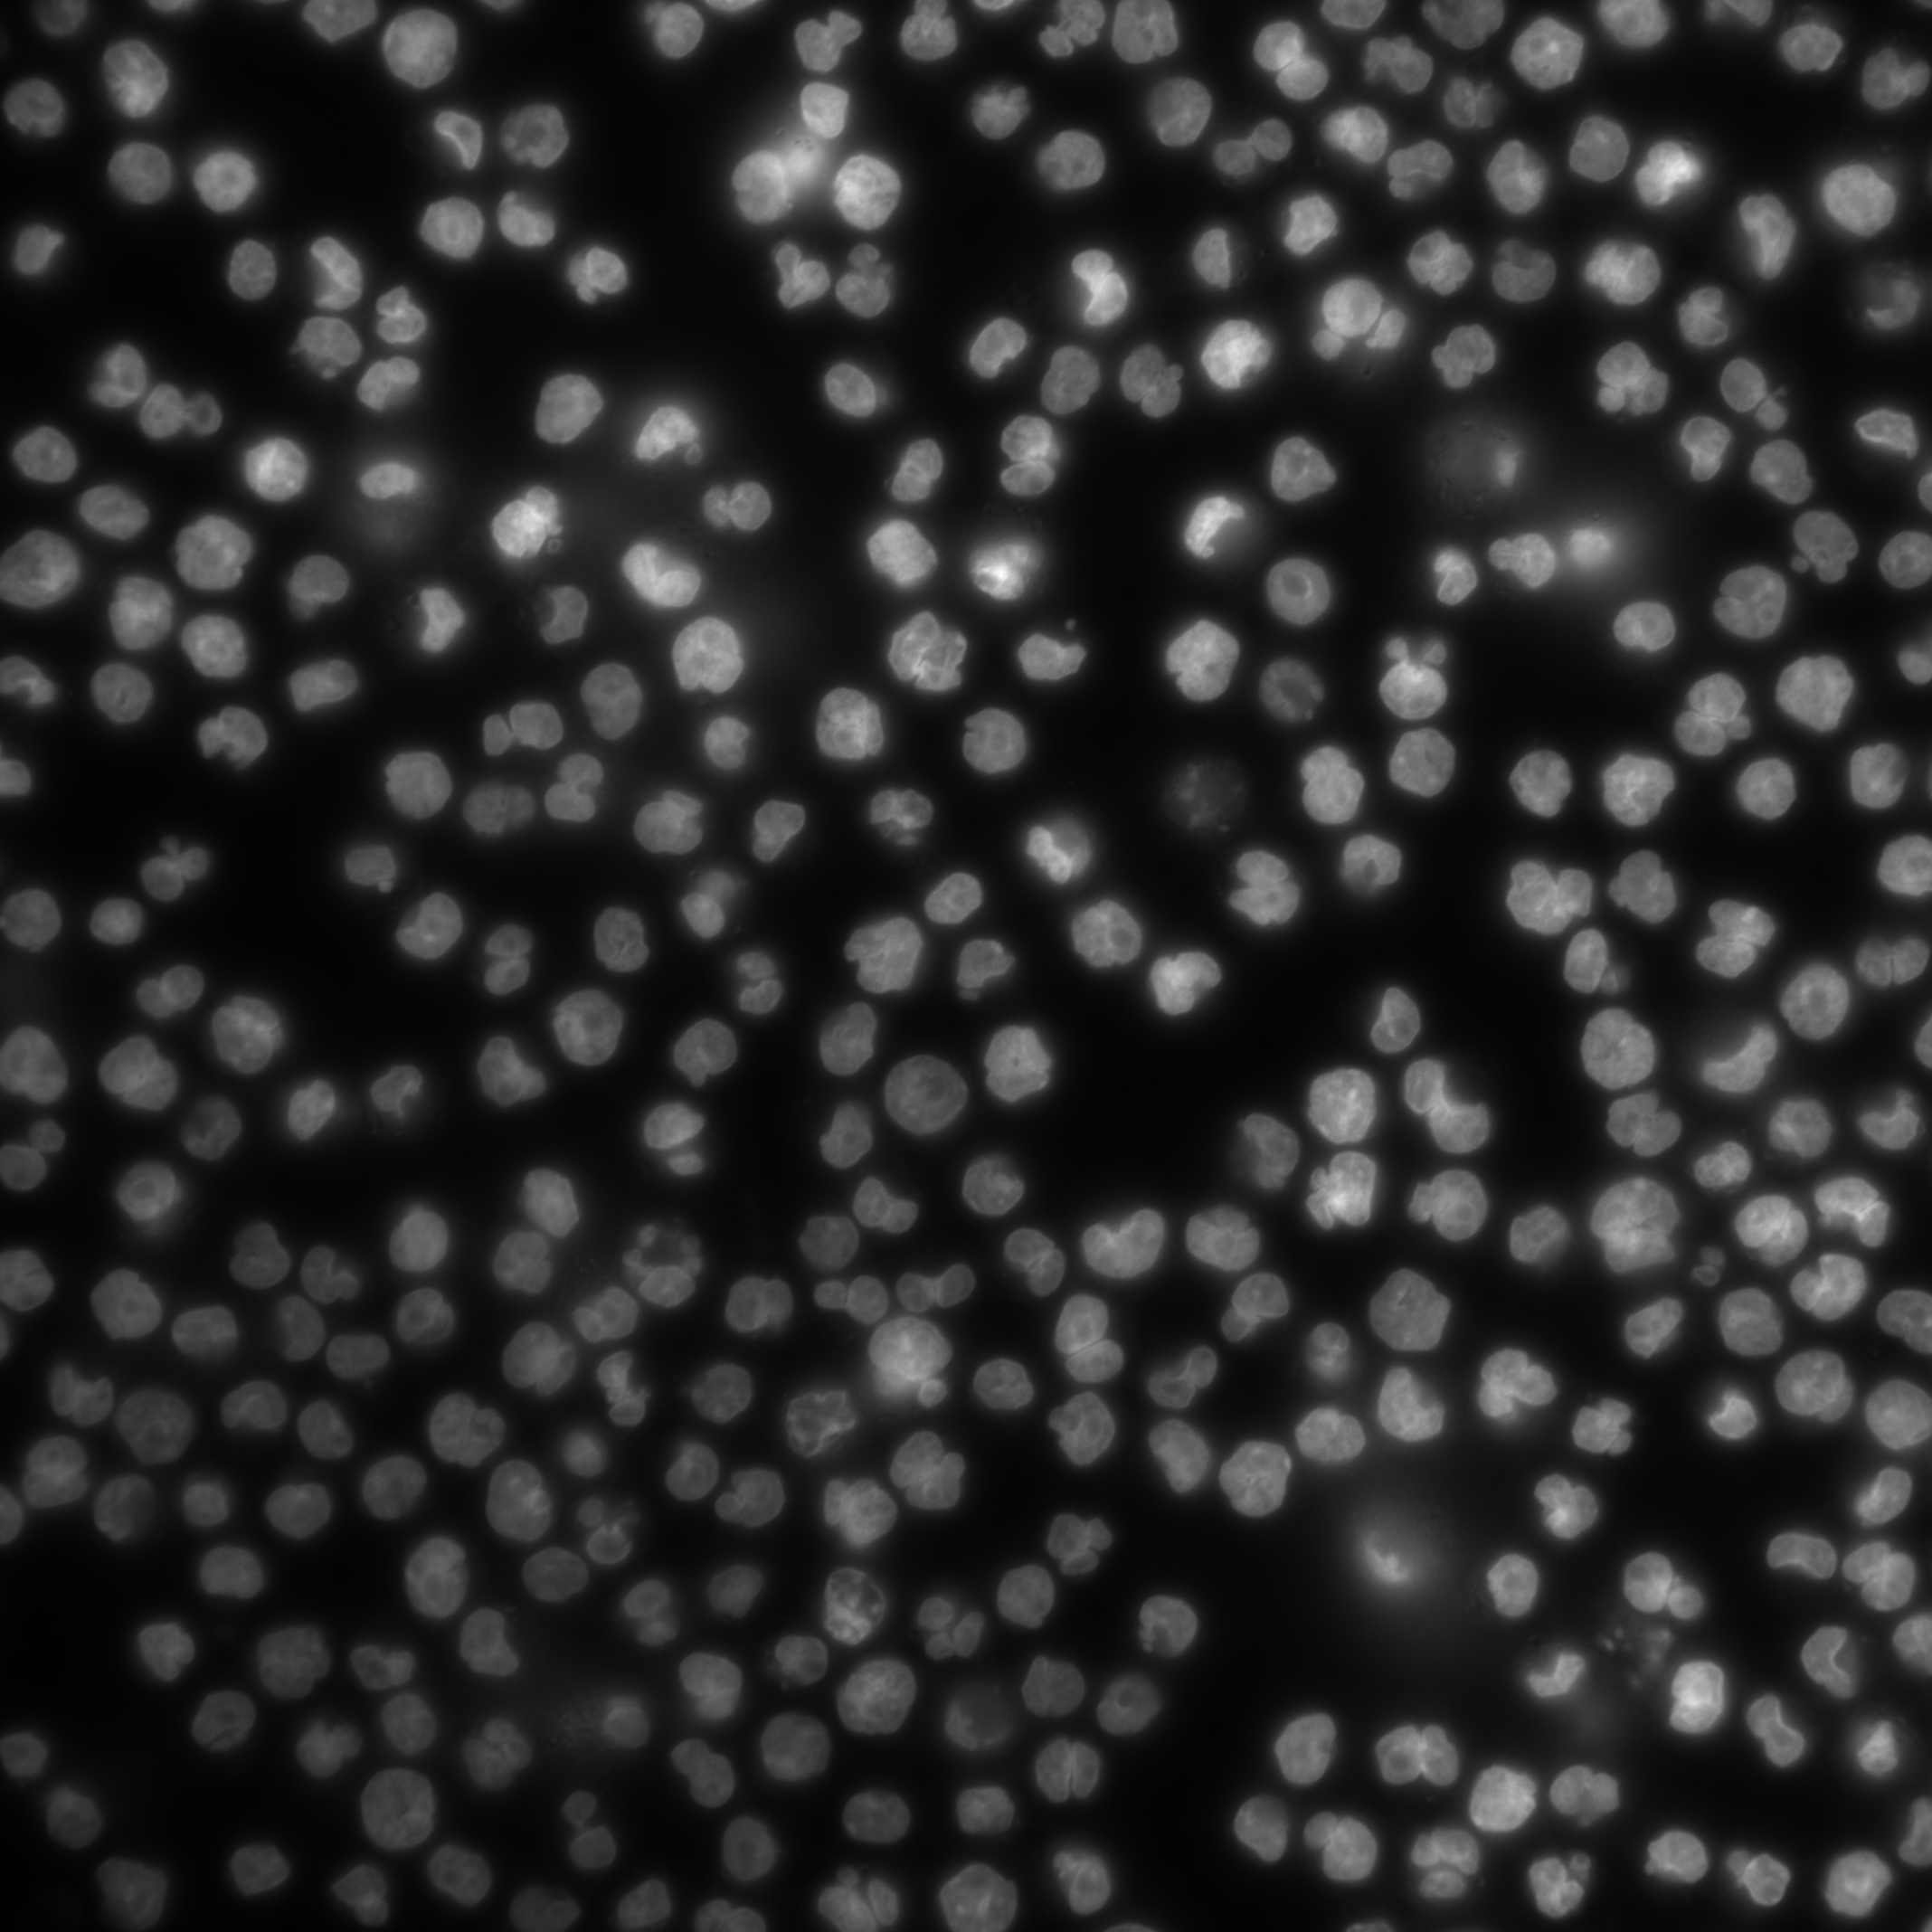
\includegraphics{bilder/lightning-conditions/lightning-3.png} &
            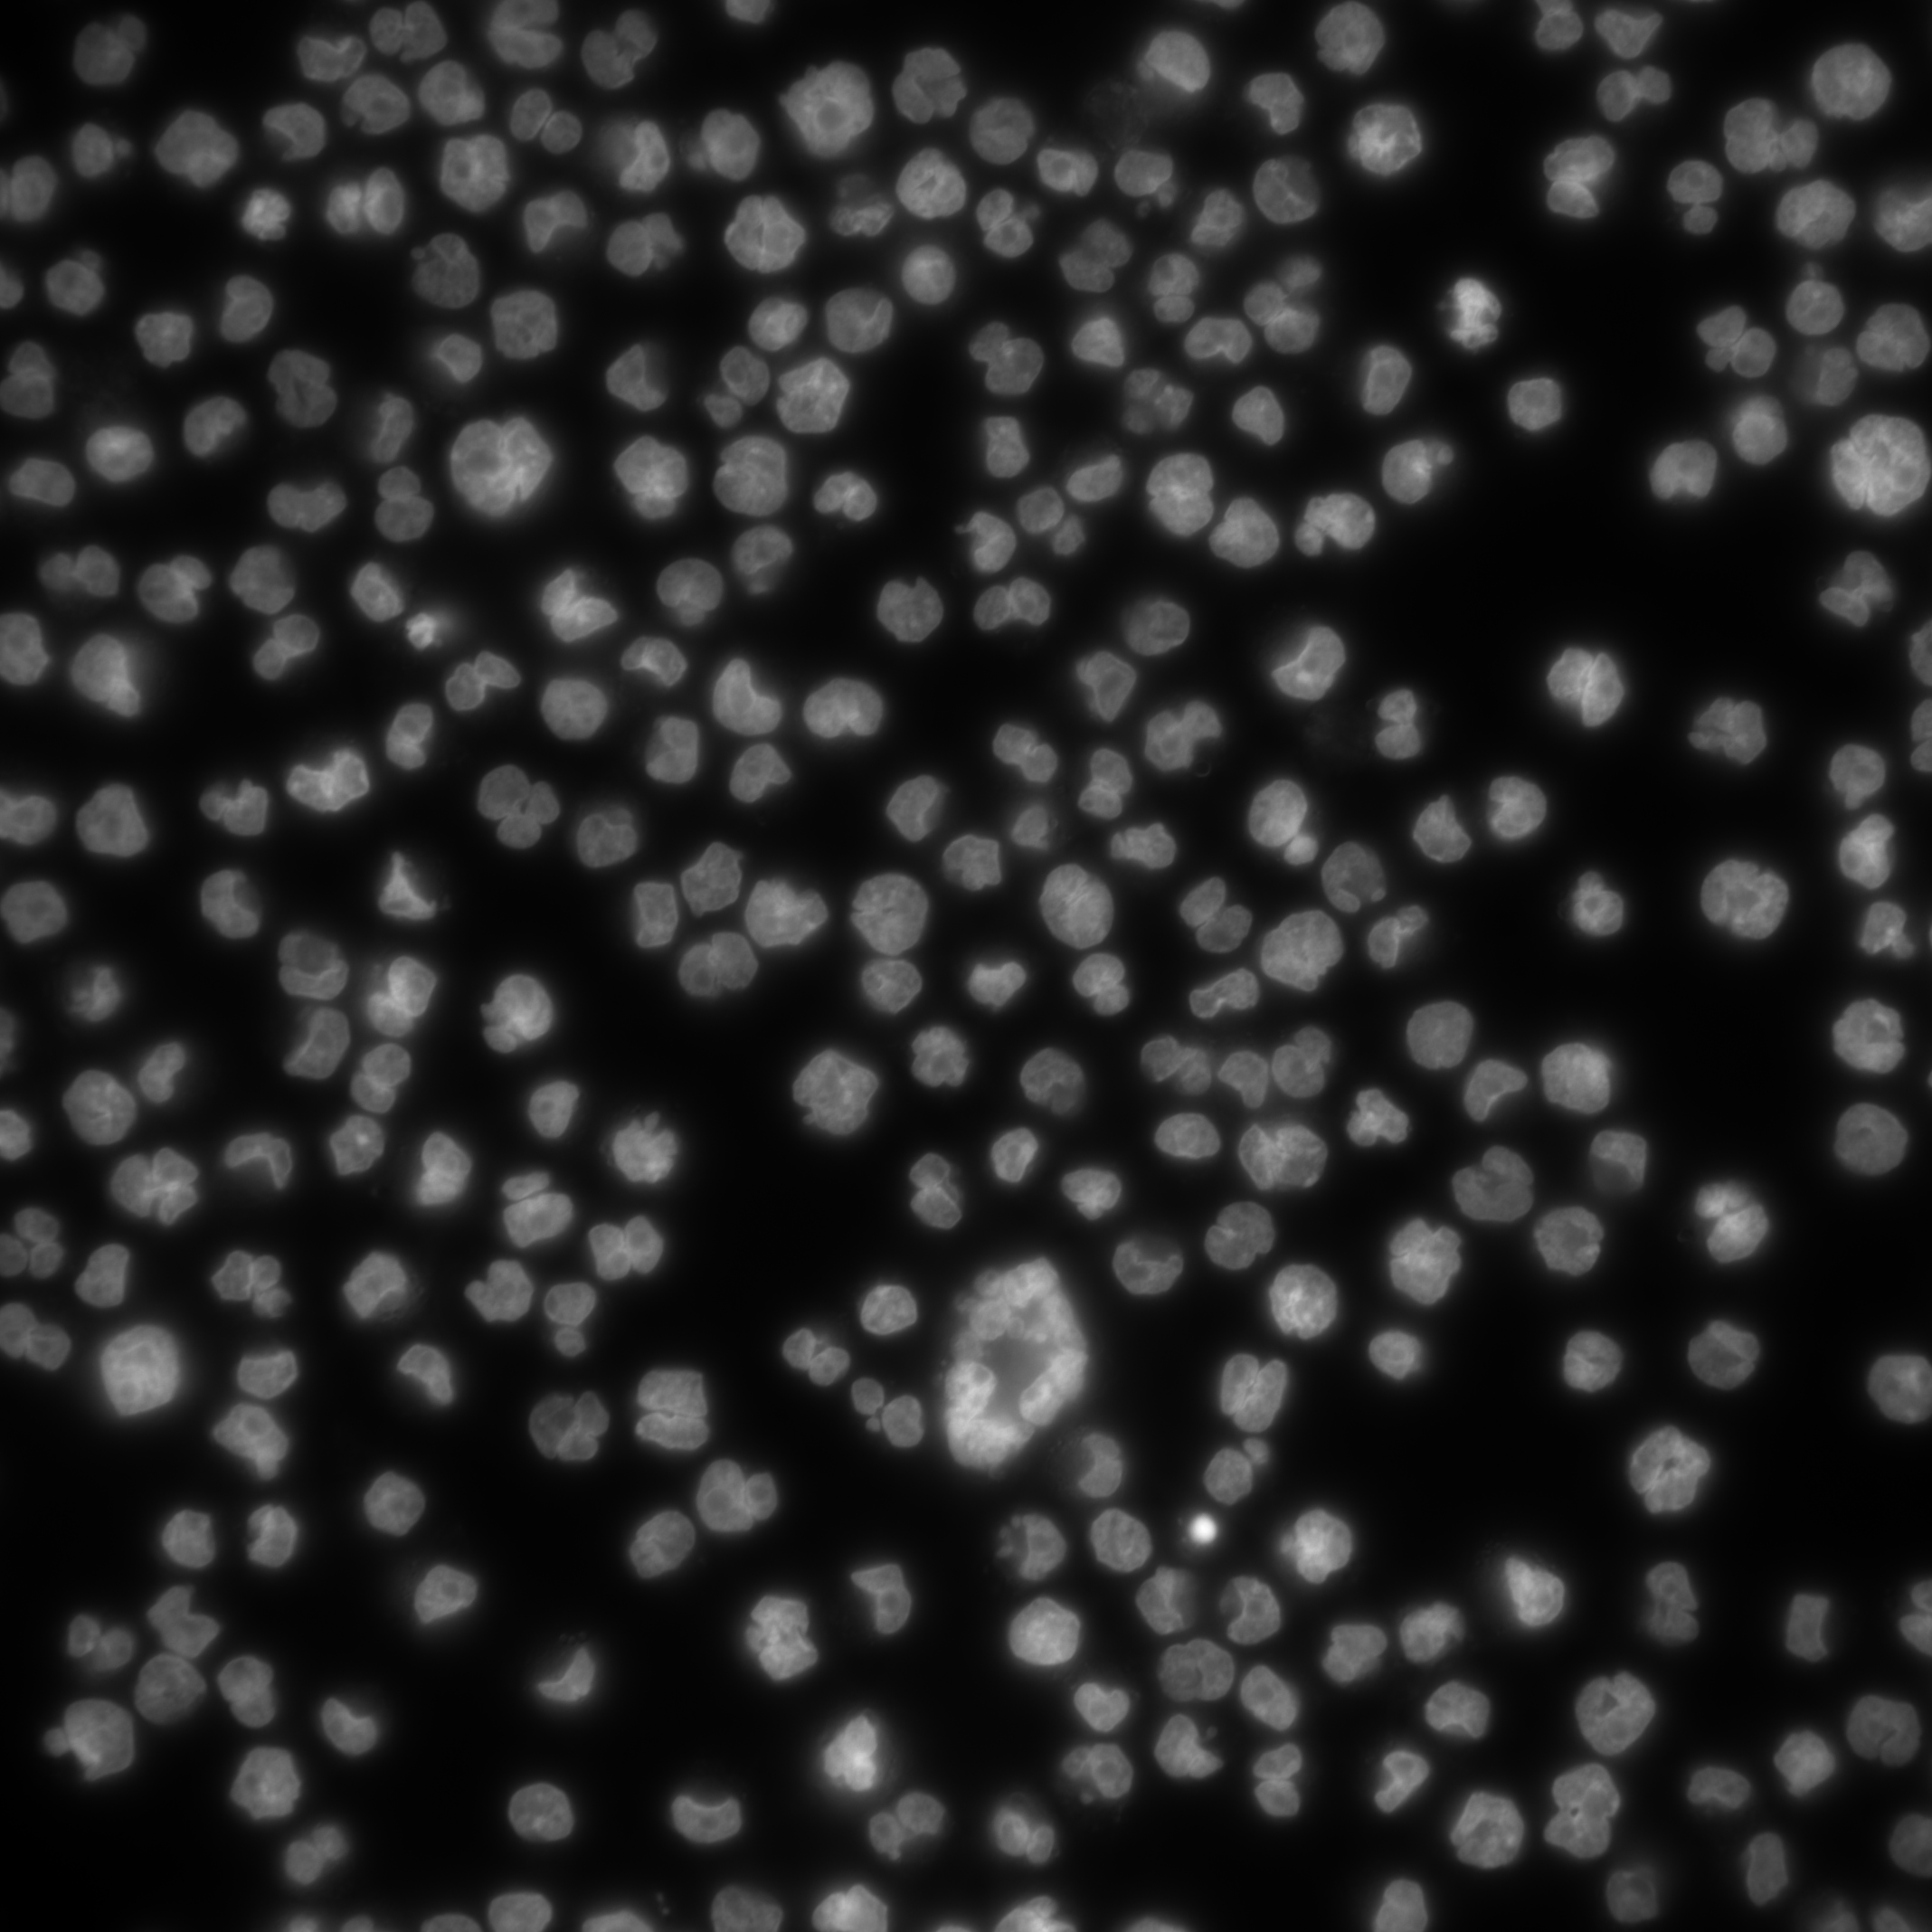
\includegraphics{bilder/lightning-conditions/lightning-4.png}
        \end{tabularx}
    \caption[Different lighting conditions]%
    {Different challenges in lightning and cells density that do not permit a successful use of a global thresholding for the foreground segmentation.}
    \label{fig:lightning_conditions}
\end{figure}

Examples of cases difficult for segmentation are presented in Figure \ref{fig:lightning_conditions} from left to right: the first image there are too few cells, which leads to the background being much darker than usual; the overexposure of one cell leads to difficulties segmenting the rest of the cells as they are hard to distinguish from the background; lighting gradient from darker (bottom left corner) to brighter (top right corner) region; normal lighting conditions.

Another challenge for segmentation bring nuclei that are very close to each other. This might happen sometimes because some of the cells are currently in the process of division. Also, when some have already fully divided, they might still be located close to one another. The example of such situations is presented in Figure \ref{fig:closely-located-cells}.

\begin{figure}[htb]
    \centering
    \subfloat[Original fluorescence]{{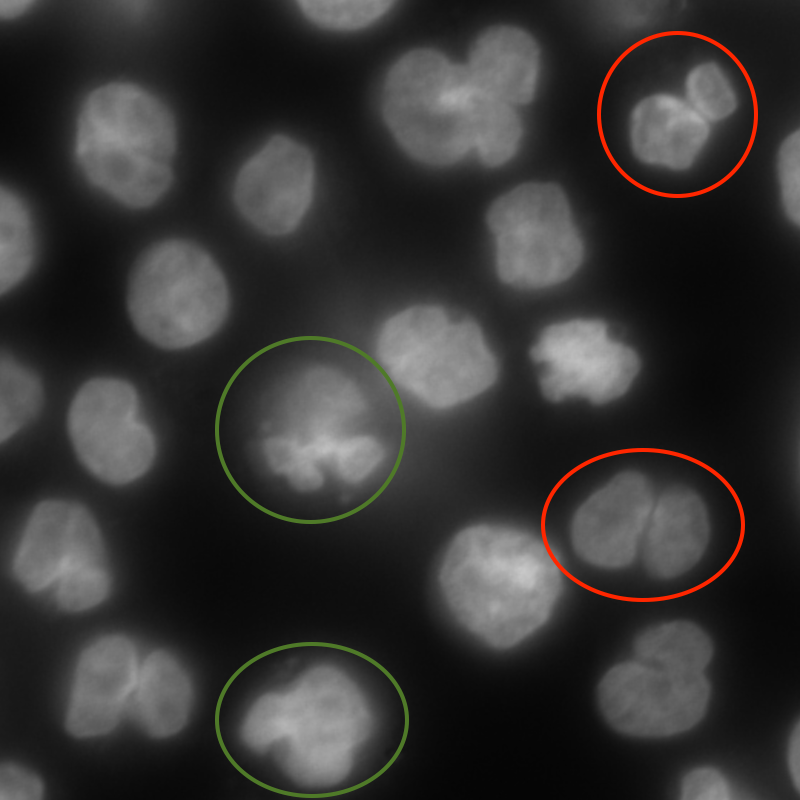
\includegraphics[width=0.2\linewidth]{bilder/close-located-cells/original.png} }}
    \qquad
    \subfloat[Segmentation (violet mask)]{{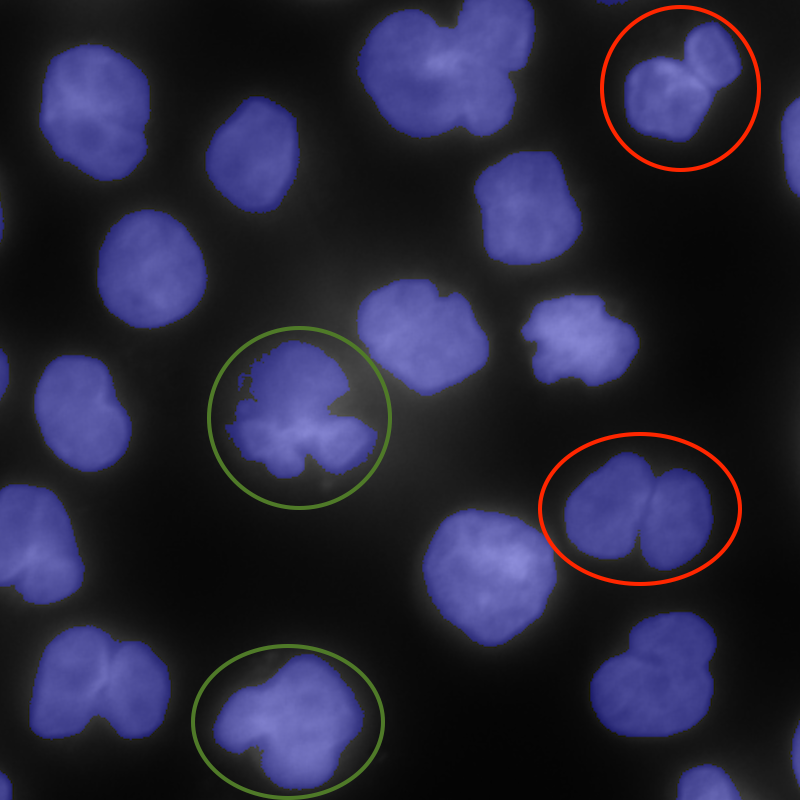
\includegraphics[width=0.2\linewidth]{bilder/close-located-cells/segmented.png} }}
    \caption[Closely located (red) and dividing (green) cells]%
    {Closely located (red) and dividing (green) cells represent a challenge for a foreground segmentation as they are recognized as one cell.}
    \label{fig:closely-located-cells}
\end{figure}

Here, the cells that are not yet fully divided are highlighted with green circles and the ones that are fully divided, but located too close to one another, are highlighted with red circles. You can see that the segmentation algorithm (see Algorithm \ref{algorithm:nuclei-segmentation}) recognises both such cases as one nucleus. This algorithm is described below and its steps are visualized in Figure \ref{fig:segmentation-nuclei-steps}.
\begin{algorithm}
    \caption{Fluorescence segmentation of nuclei}
    \begin{algorithmic}
    \item 1. Normalize image.
    \item 2. Apply local thresholding and get a threshold $T$ or a set of local thresholds \{$T_i$\} and create an initial mask: $1$ if $x_i > T$ or $0$ otherwise.
    \item 3. Apply \textit{fill\_holes} transformation to the initial mask in order to get rid of unneeded details within the nuclei.
    \item 4. Run \textit{findContours} from opencv in order to obtain separate regions and filter them based on the following criteria: filter out regions that are too big (measure the biggest possible nuclei manually), regions that are too small (measured manually as well), regions that have a shape that is not similar to convex circular type of nuclei. The last filter is done by checking the ratio of the area of the region to the area of the convex hull of the region (for more details regarding \textit{findContours} implementation refer too \cite{Suzuki_1985}).
    \end{algorithmic}
    \label{algorithm:nuclei-segmentation}
\end{algorithm}

\begin{figure}[htb]
    \centering
    \setkeys{Gin}{width=\linewidth}
    \centering
        \begin{tabularx}{\textwidth}{YYYY}
            \textbf{Normalized input} &
            \textbf{Local threshold} &
            \textbf{Filled holes} &
            \textbf{Filtered regions} \\
            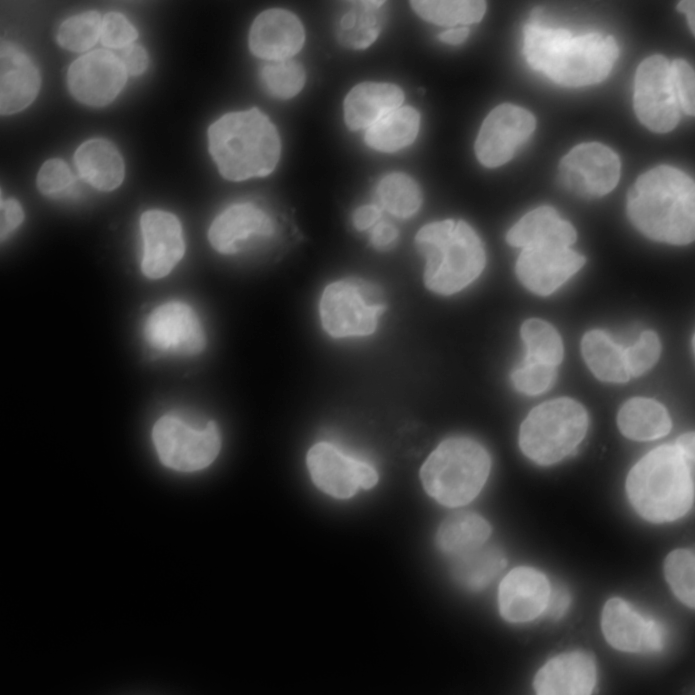
\includegraphics{bilder/segmentation/nuclei-mask/normalized.png} & 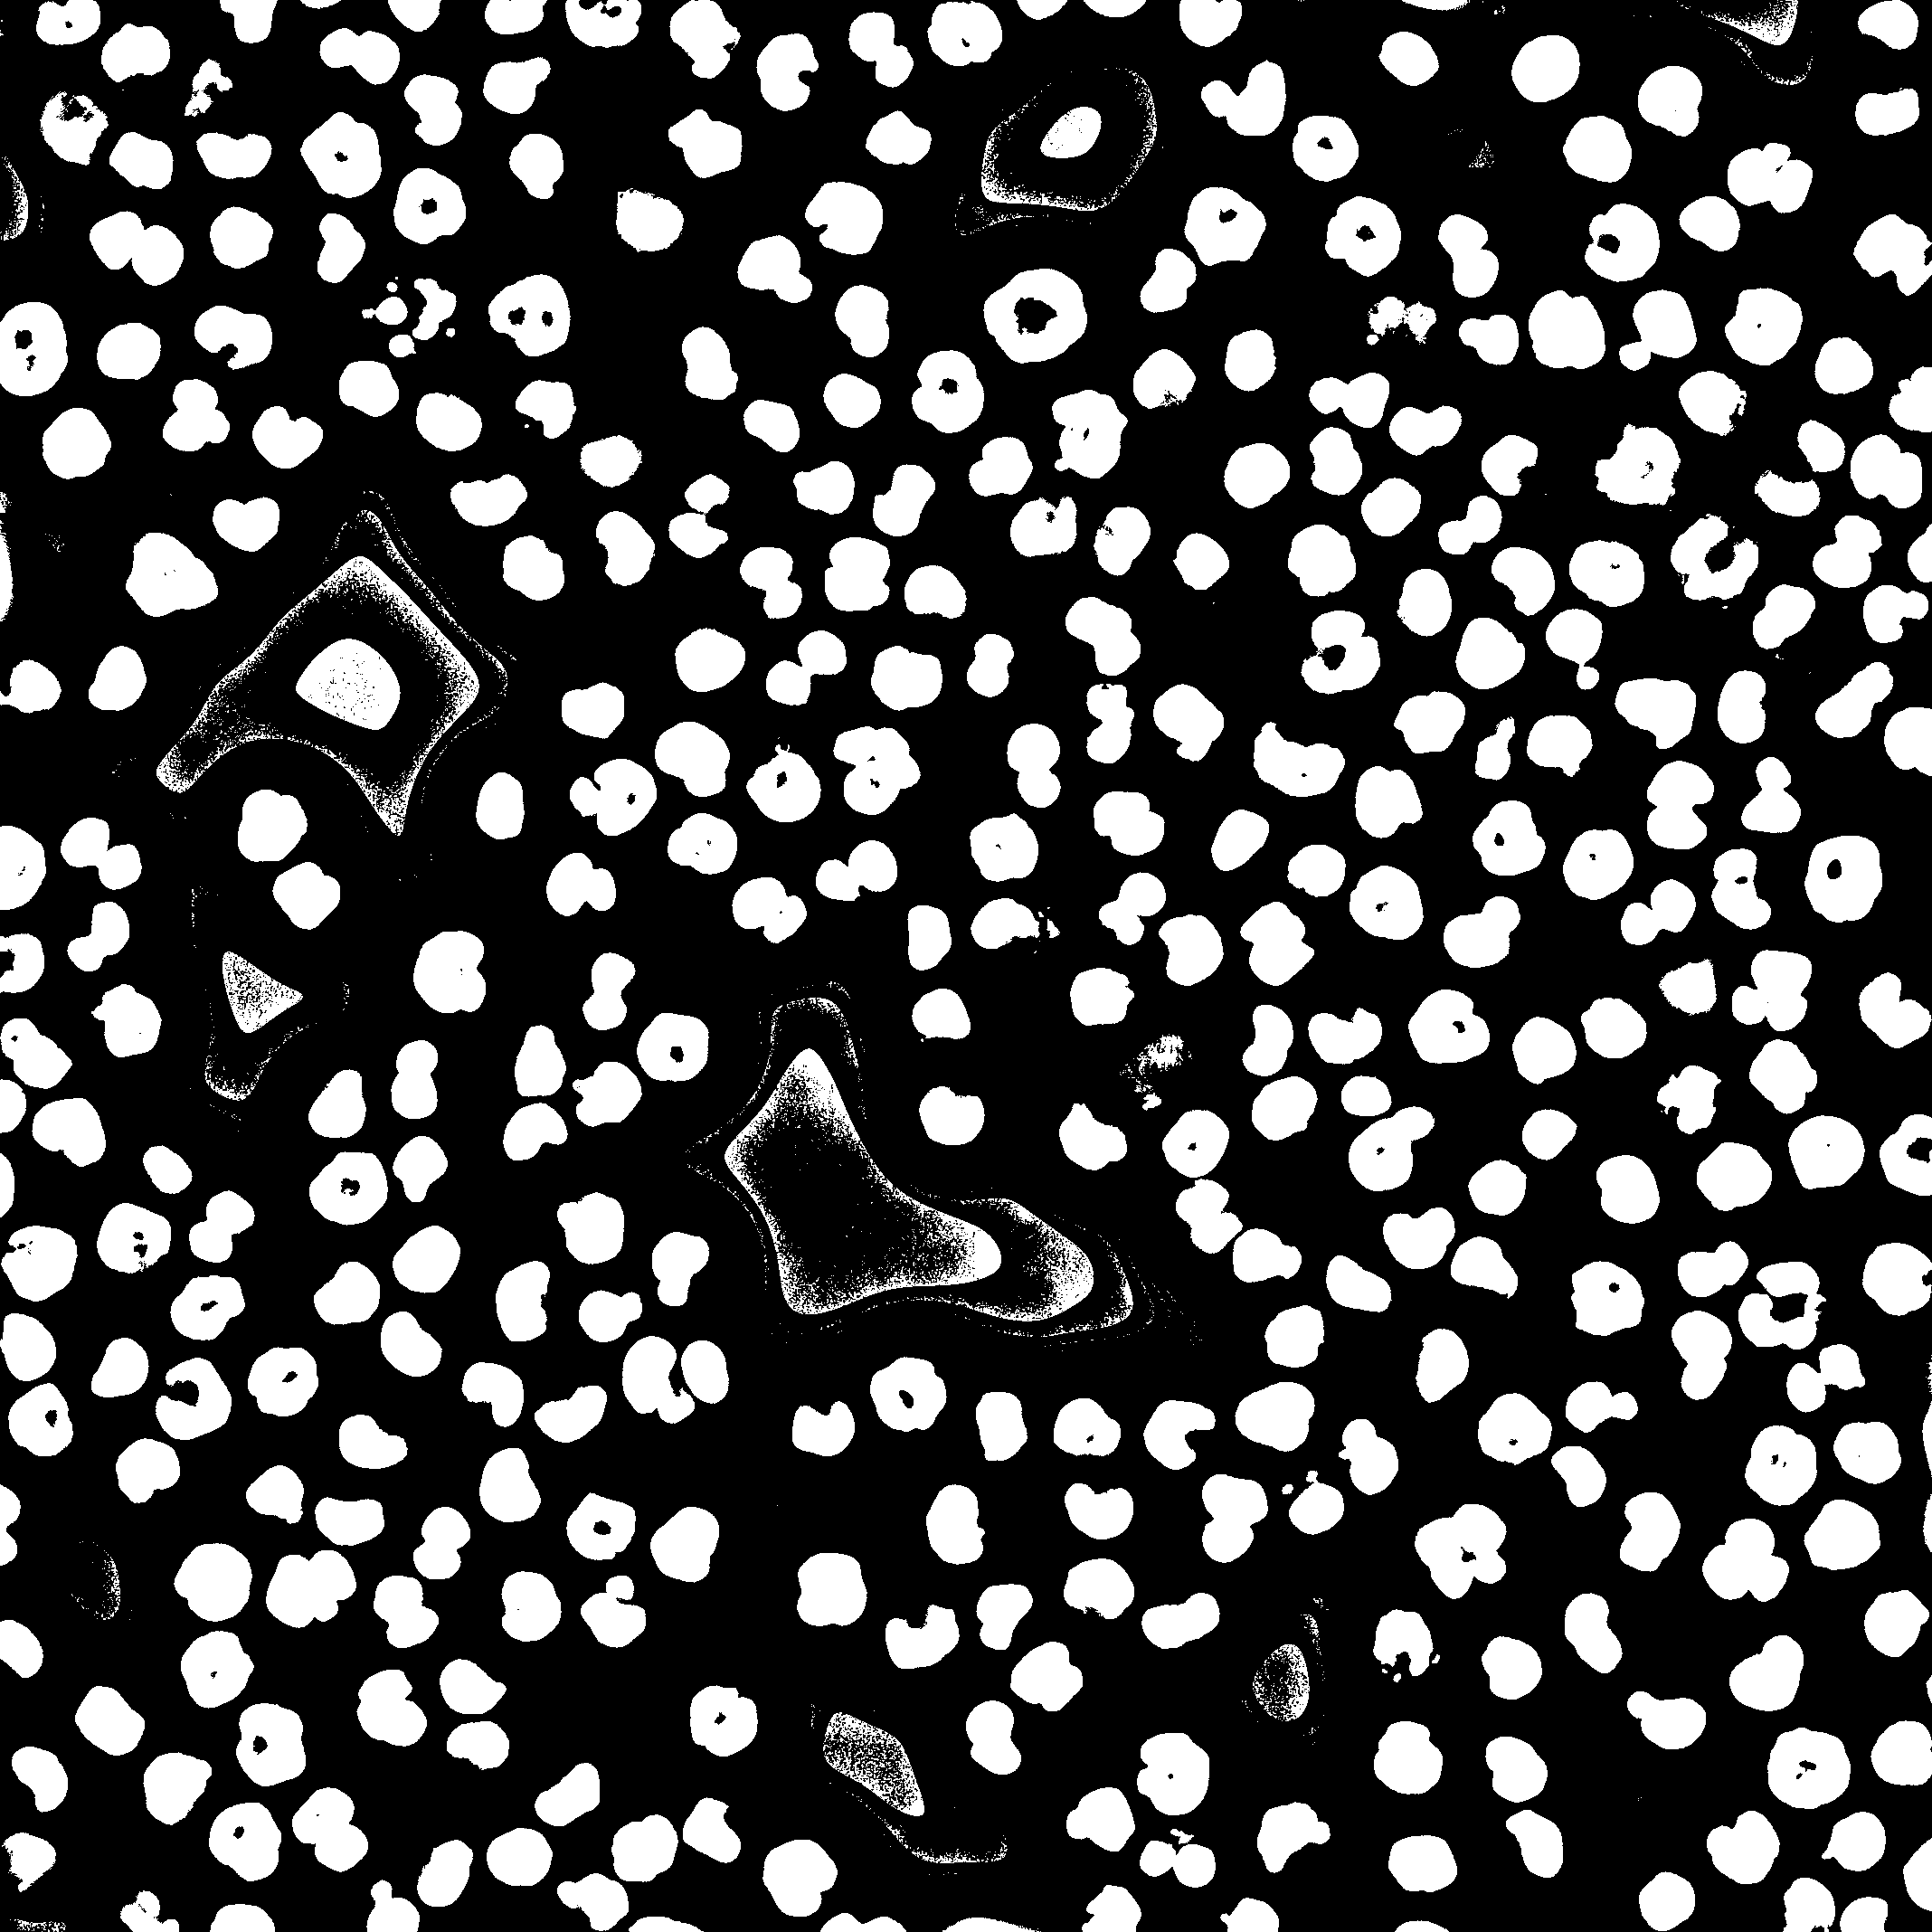
\includegraphics{bilder/segmentation/nuclei-mask/binary_local.png} &
            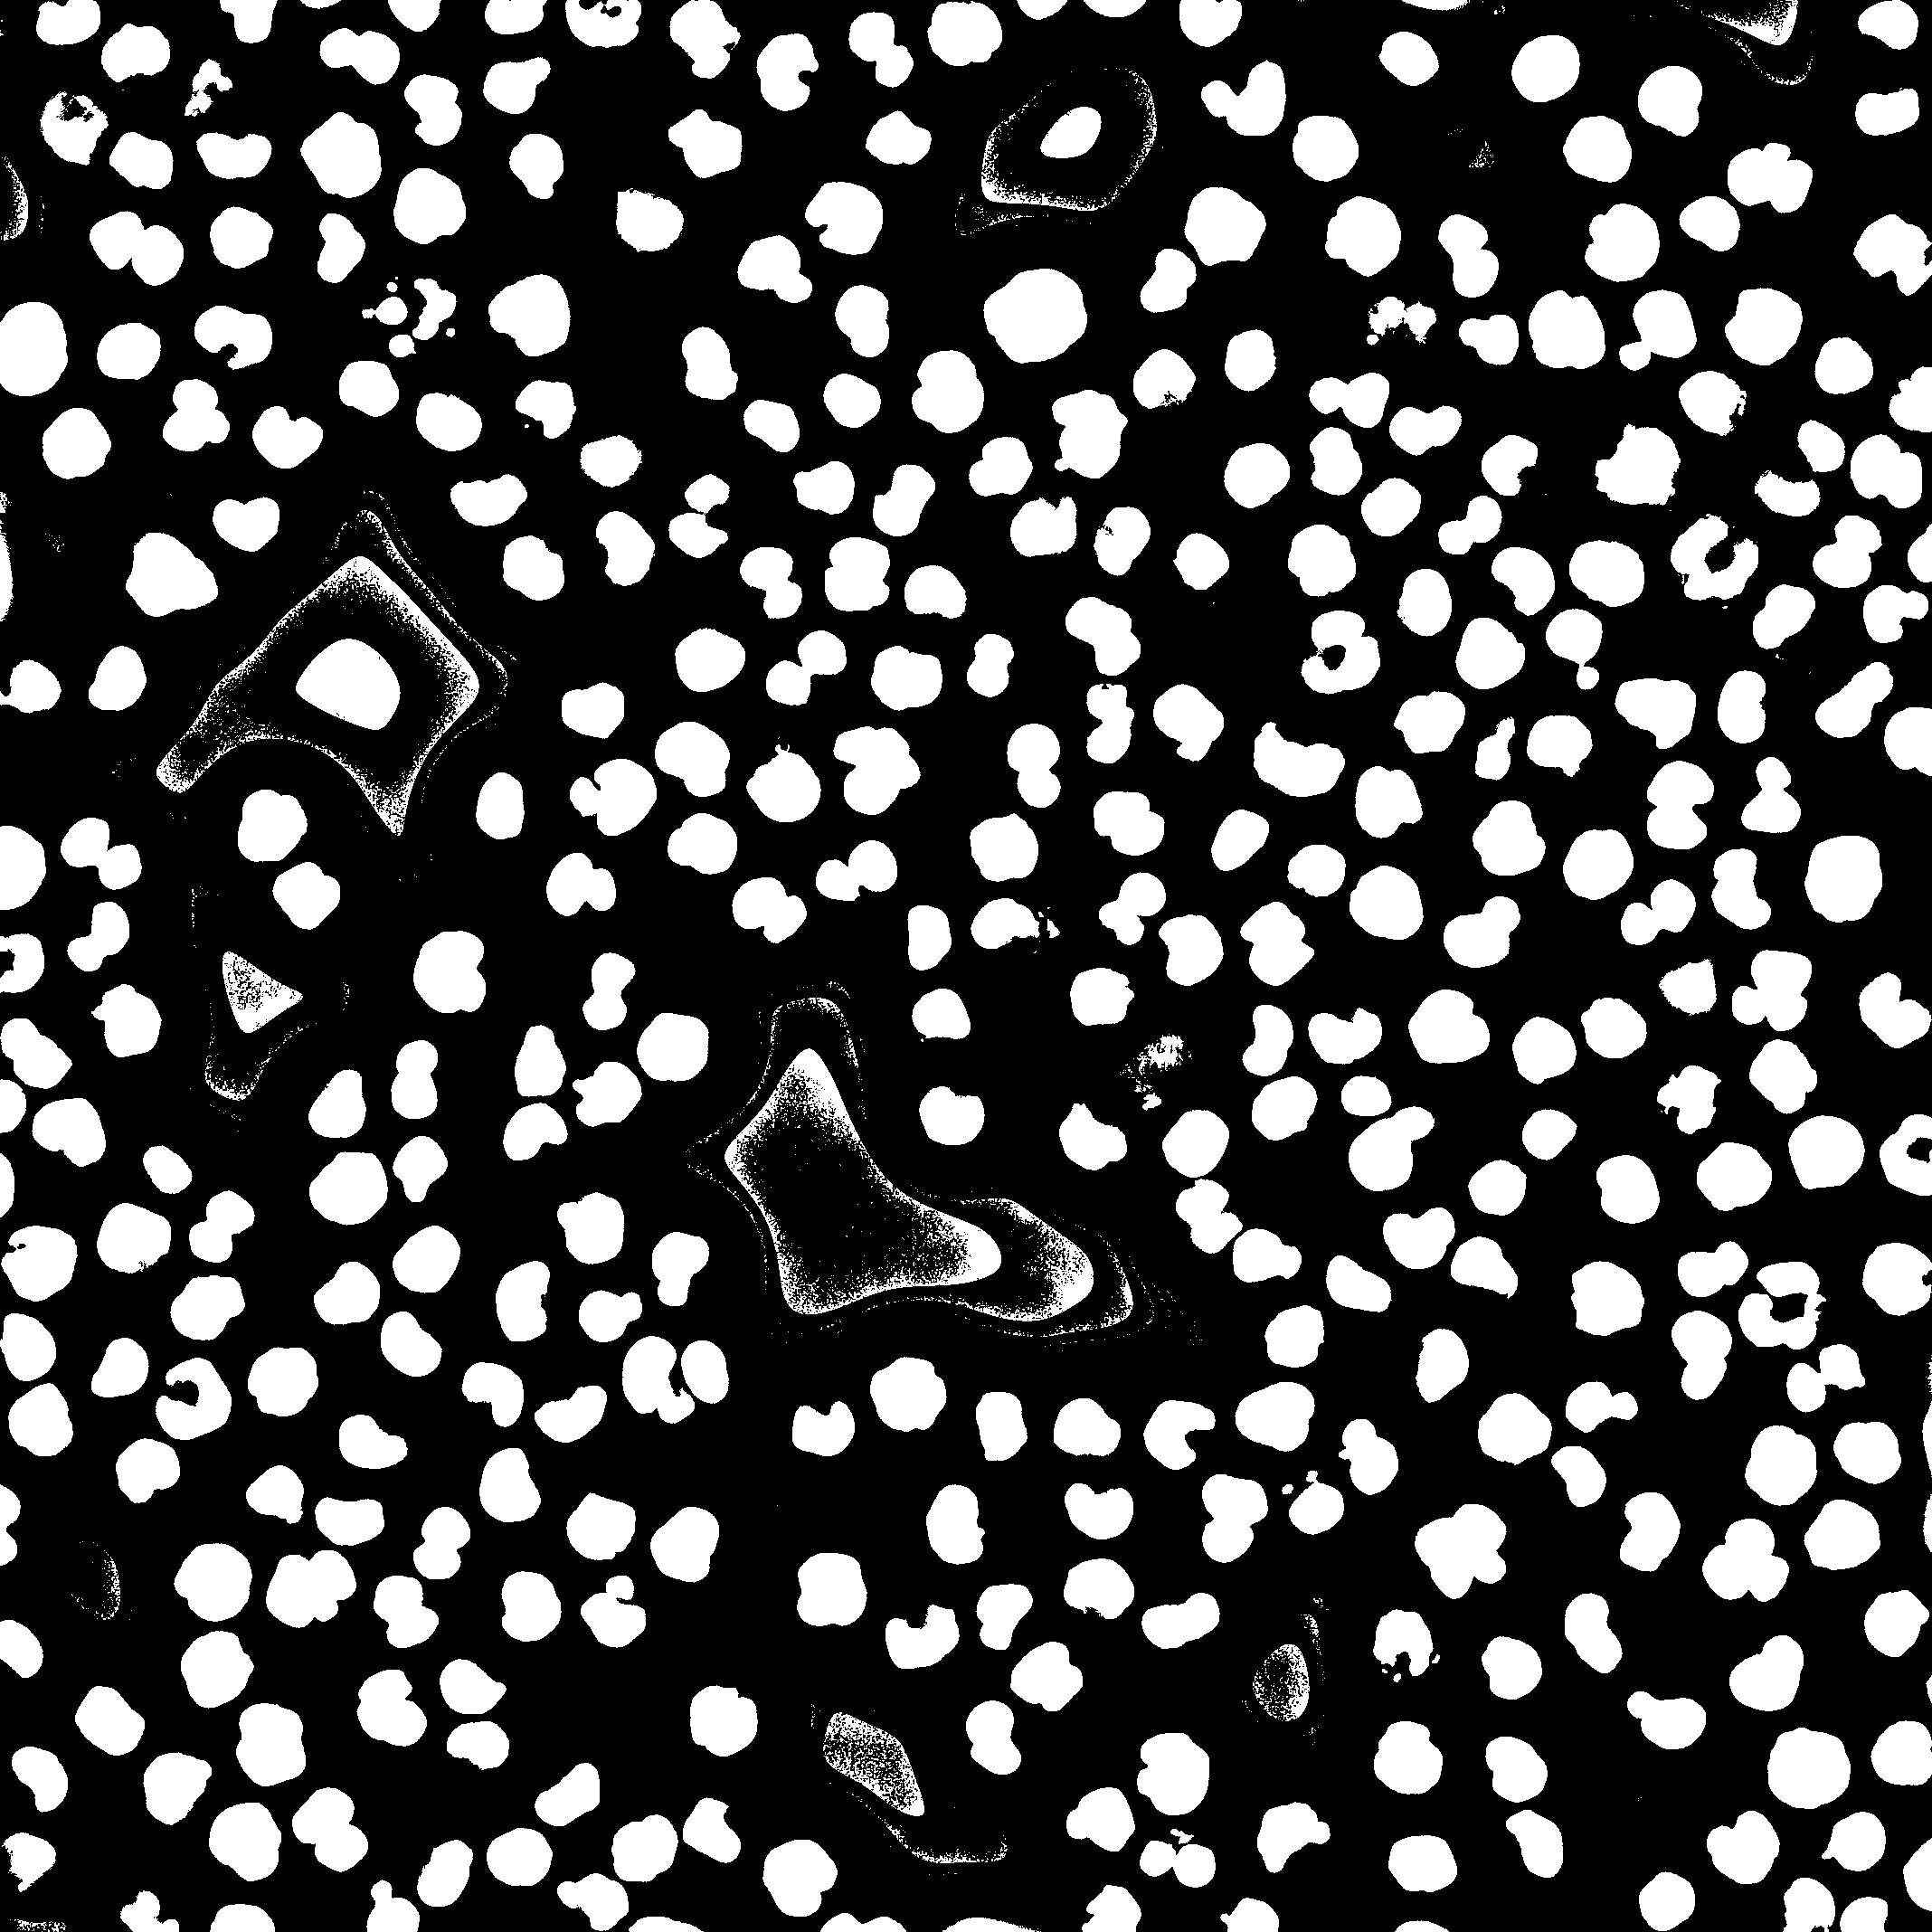
\includegraphics{bilder/segmentation/nuclei-mask/filled_holes.png} &
            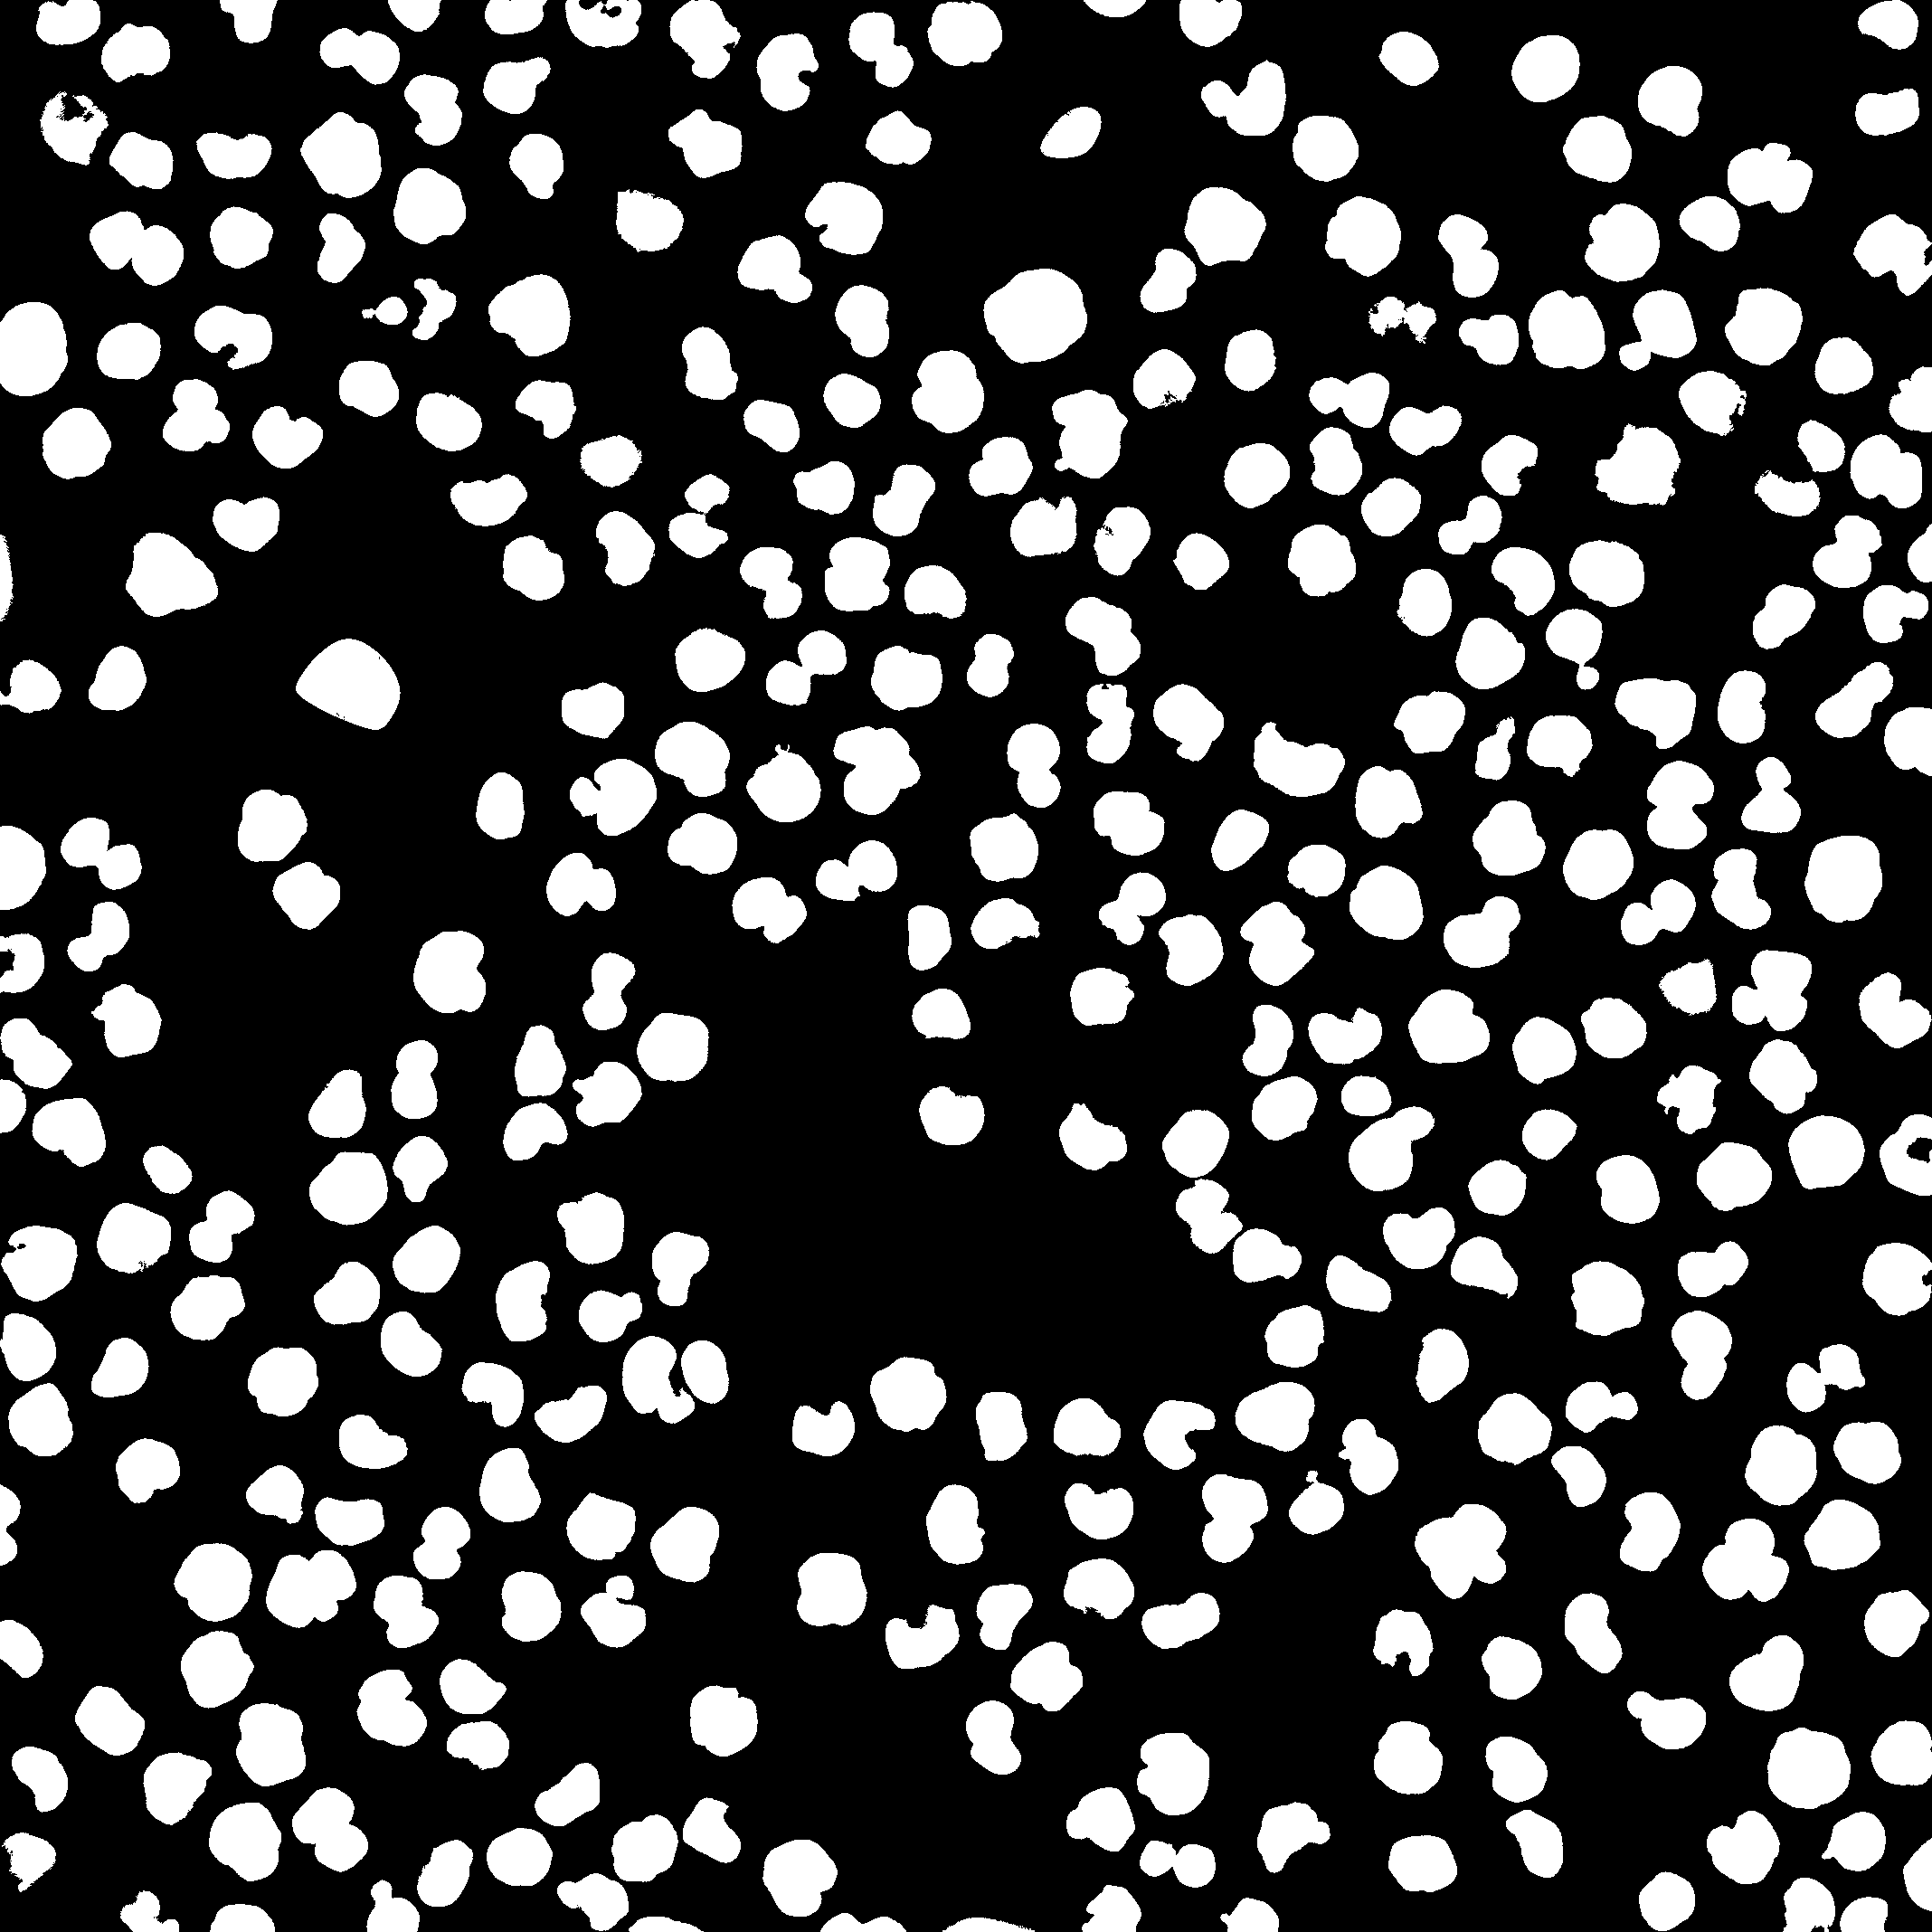
\includegraphics{bilder/segmentation/nuclei-mask/mask.png}
        \end{tabularx}
    \caption[Fluorescence segmentation]%
    {Fluorescence segmentation. Artifacts of local thresholding algorithm visible in the second image can be successfully filtered out based on their shape.}
    \label{fig:segmentation-nuclei-steps}
\end{figure}

A more detailed description of the reasoning why local thresholding approach was chosen is provided in the following subsection.

        \paragraph{Thresholding algorithms}
        There are in general two types of thresholding that exist to binarize an image (create its mask): global and local.

\textbf{Global thresholding} is a an algorithm that simply choses one threshold $T$ for the whole histogram of the image. All pixels that are smaller than this threshold $x_{i,j} < T$ are assigned to be of class $0$ (background) and all pixels that are larger than this threshold $x_{i,j} > T$ are assigned to be of class $1$ (foreground). It is very difficult to find a good threshold manually that would work out for all the images, especially in this case, when the brightness does differ not only between the images, but also within the image itself (light gradient in Figure \ref{fig:lightning_conditions}). To find a good threshold automatically (at least to some extect) \cite{digital_image_book} proposed the following algorithm:

\begin{algorithm}
  \caption{Global thresholding}
  \begin{algorithmic}
    \item 1. Select an initial estimate for $T$.
    \item 2. Segment the image using T. This will produce 2 groups of pixels $G_1$ (all pixels $x_i > T$) and $G_2$ (all pixels $x_i < T$).  
    \item 3. Computer the average gray values $\mu_1$ and $\mu_2$ for the pixels in  regions $G_1$ and $G_2$.
    \item 4. Compute a new threshold value 
        $T' = \frac{\mu_1 + \mu_2}{2}$
    \item 5. Repeat steps 2-4 until difference in the change of value $T$ is smaller that a predefined parameter.
  \end{algorithmic}
  \label{alg:global-thresholding}
\end{algorithm}

Nevertheless, it is not obvious how to preselect an initial threshold in step 1. There are several options here, however keep in mind that there is also no single best solution among them. For example, when an assumption that the foreground occupies approximately the same area as the background holds, than initial threshold $T$ should be chosen to be an average gray level and etc.

After trying out many different global threshold approaches, it has been derived that a \textit{global minimum thresholding} is the best one. It is implemented in \textit{skimage.filters} and according to the documentation (\cite{global_thresh}) works in the following way: it assumes that the histogram $p = (p_0, \ldots, p_{M})$ of the image is bimodal, meaning that it has two clearly defined peaks (background and foreground). Afetrwards the histogram is iteratively smoothed using a running average of size $k=3$. The points on the histogram are updated with the value $a_k$ from Equation \ref{eq:SMA} until only 2 local maximas ($a_l$ and $a_r$) are left. 
\begin{equation}
    a_k = \frac{1}{k}\sum_{i=n-k + 1}^{n}p_i
\label{eq:SMA}
\end{equation}
Then the threshold is taken as the minimum between the two local maximas:
\begin{equation}
    a_l \leq T \leq a_r
\end{equation}

One clear downside of this approach though is that images which histograms have very unequal peaks or a broad and flat valley will be unsuitable for this method (\cite{thresholding_skimage}).

\begin{figure}[htb]
	\begin{center}
		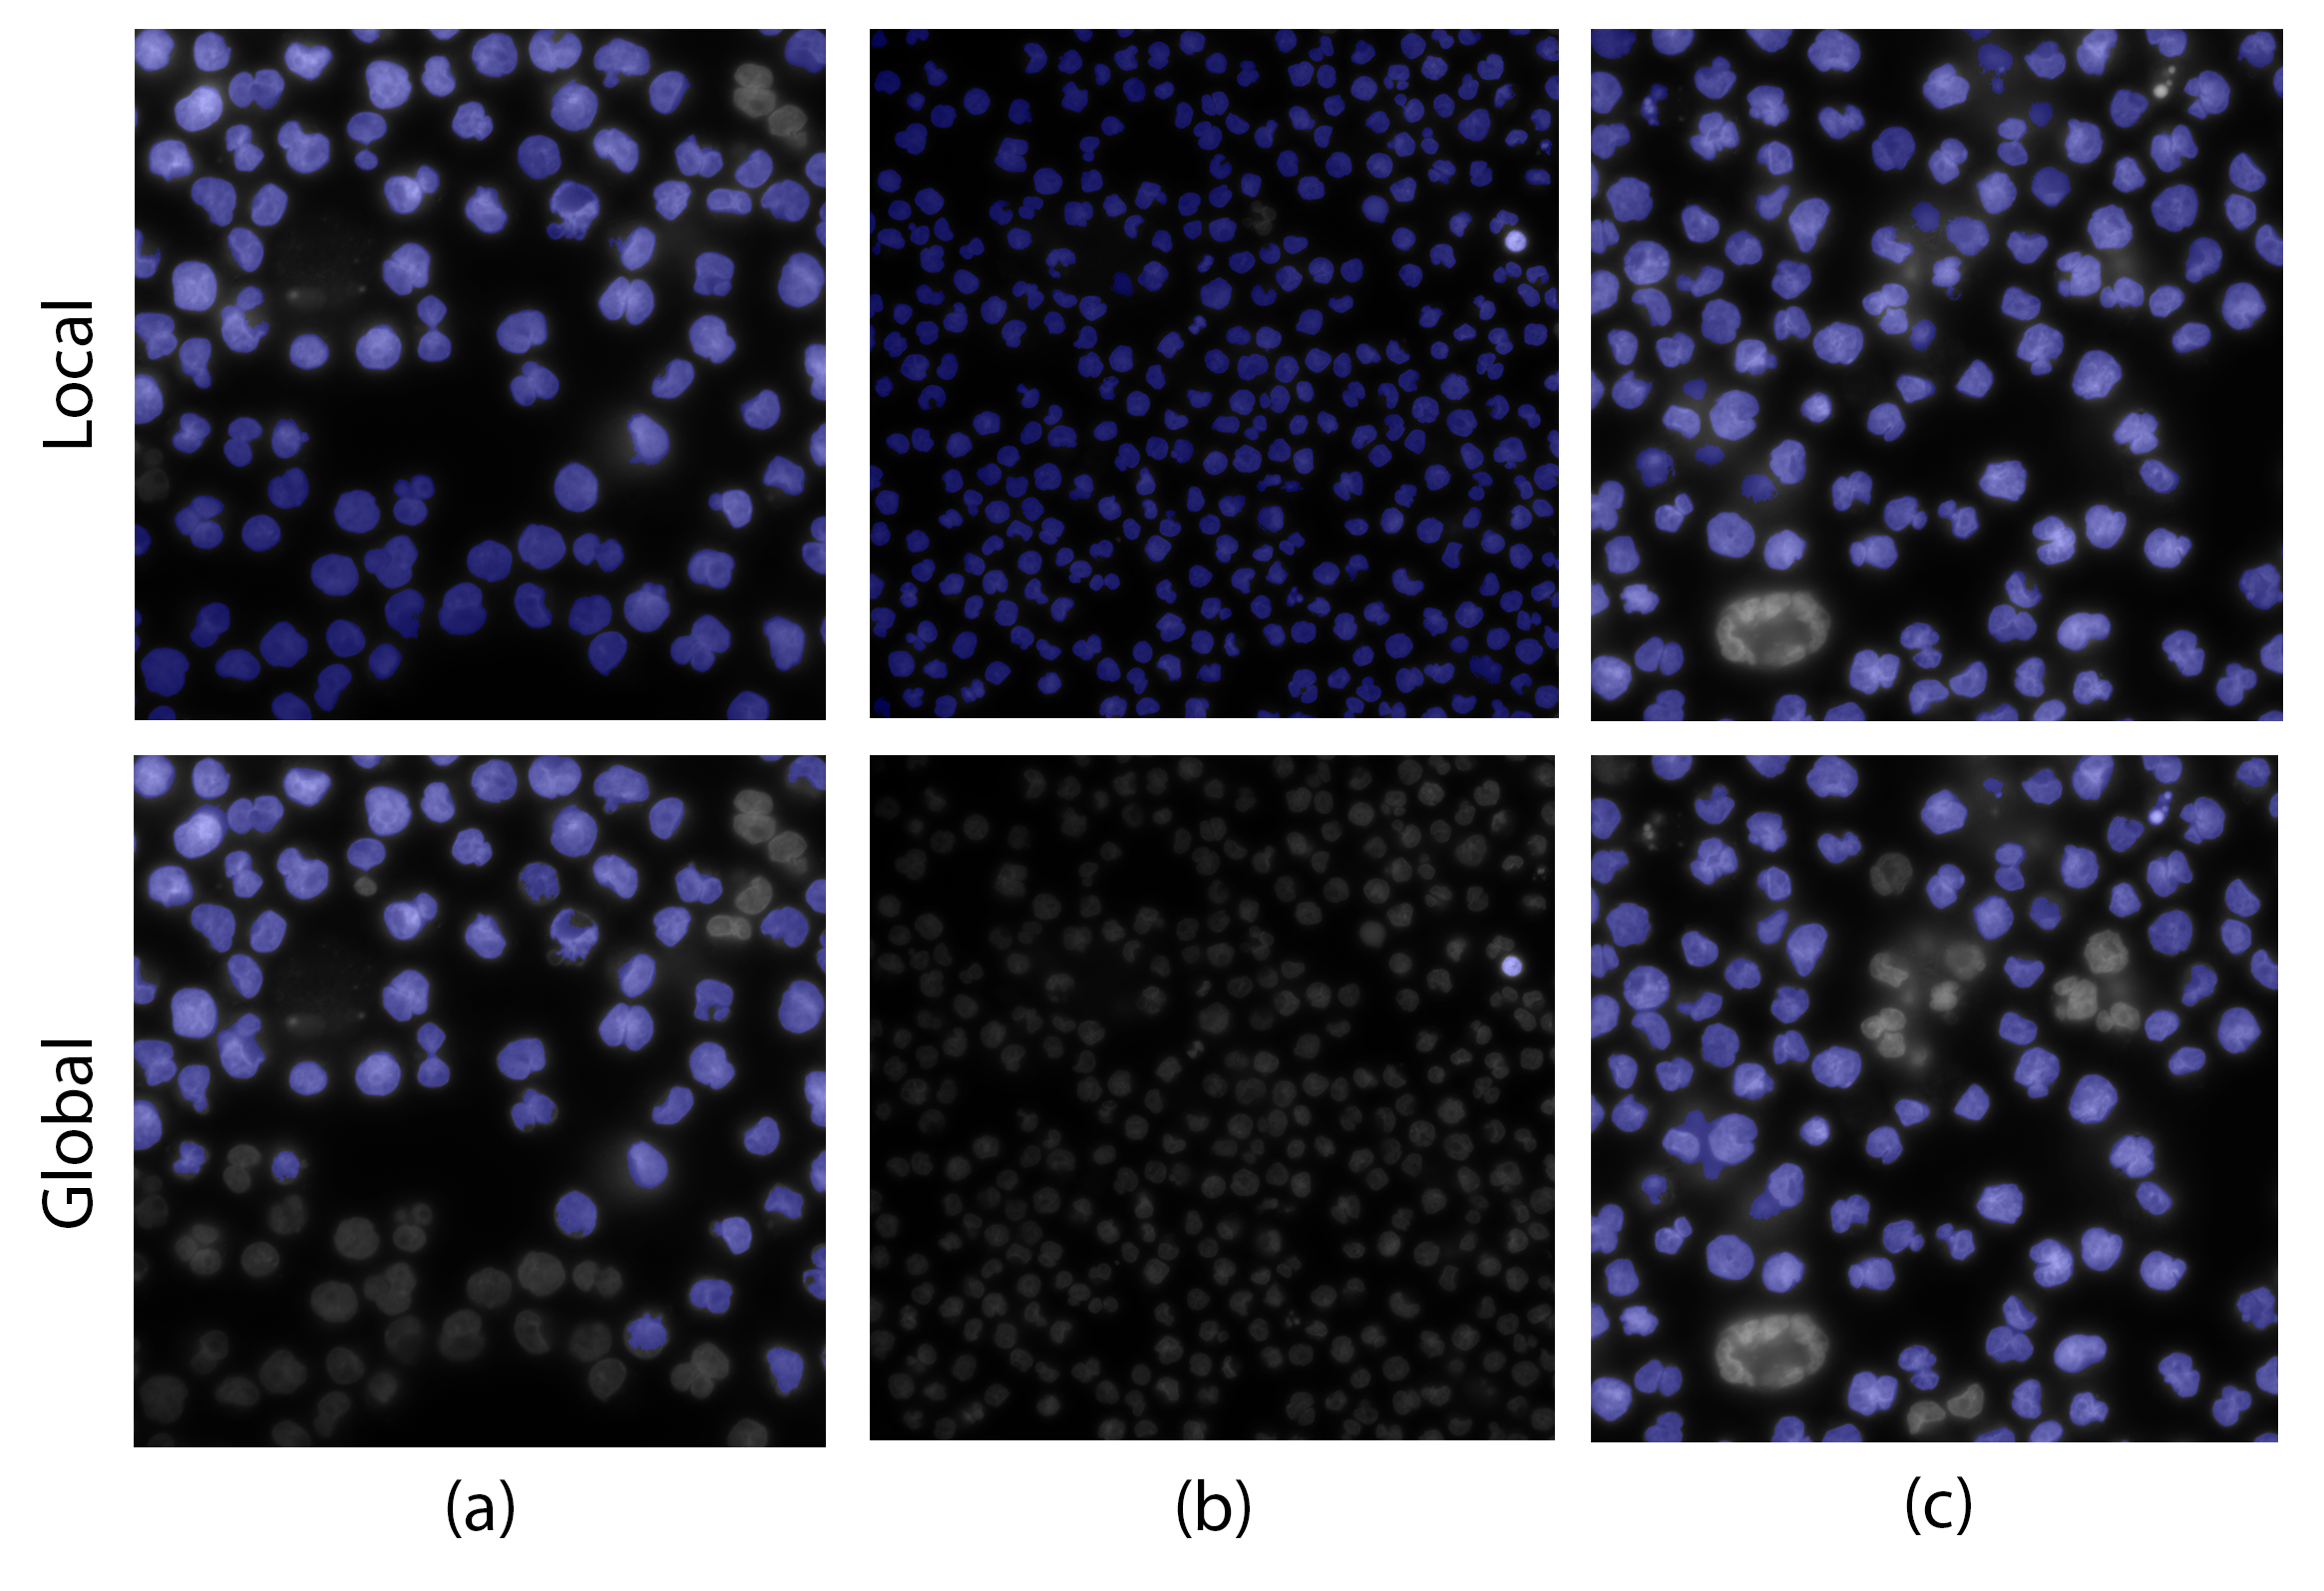
\includegraphics[width=0.6\linewidth]{bilder/difficult-lightning/local-vs-global.png}
		\caption{Local vs. global thresholding}\label{fig:thresholding-bad-conditions}
	\end{center}
\end{figure}

Unfortunately this method did not perfom well even for the images that have an equal amount of foreground and background. And the reason for that is a mentioned above non-uniform illumination within the images. For visual comparison of global thresholding applied to difficult images see Figure \ref{fig:thresholding-bad-conditions}a, b, c Global. \ref{fig:thresholding-bad-conditions}c is an image with equal brightness level, however even there some mistakes do appear.

However there is another better approach that performs well in such conditions: \textbf{local thresholding}. For nuclei segmentation exactly this algorithm was chosen. It is implemented in \textit{skimage.filters} and can be used in the following way:

\begin{lstlisting}
  skimage.filters.local_threshold(img, block_size=7, method='gaussian', offset=0)
\end{lstlisting}

The main idea behind it is the following: instead of selecting one threshold for the whole image (global one), one can select several thresholds for each local region with a predefined size. The comparison between global and local thresholding is presented in Figure \ref{fig:thresholding-bad-conditions}, where (a), (b) denote exteme corruption cases and (c) represents a normal illumination.

"The threshold value is the weighted mean for the local neighborhood of a pixel subtracted by a constant (\cite{digital_image_book})". With the image size of $2136 \times 2136$, the local neighborhood (or a \textit{block\_ size}) by experimenting with different values was chosen equal to $111$. The default \textit{method} used on for local thresholding is \textit{gaussian}, \textit{offset} value is a constant that will be subtracted from weighted mean of neighborhood during the calculation of the local threshold, by default this value is $0$ \cite{local_thresholding}.

Let $z$ be a random variable that quantifies a gray-level value of the pixel, then the histogram of the image is a probability density function (PDF) $p(z)$. Since we assume that the image contains a background and a foreground, then this PDF is a mixture of two densities $p_1(z)$ and $p_@(z)$ weighted by the relative areas of these two classes (their number of pixels) $P_1$ and $P_2$. Then 

\begin{equation}
    p(z) = P_1 p_1(z) + P_2 p_2(z)
\end{equation}

By assuming Gauassian model for both $p_1(z)$ and $p_2(z)$, one gets a Gaussian Mixture Model (GMM). Since we have assumed that each pixel can be asssigned to either a background of foreground only, $P_1 + P_2 = 1$ must hold. 

\begin{figure}[htb]
	\begin{center}
		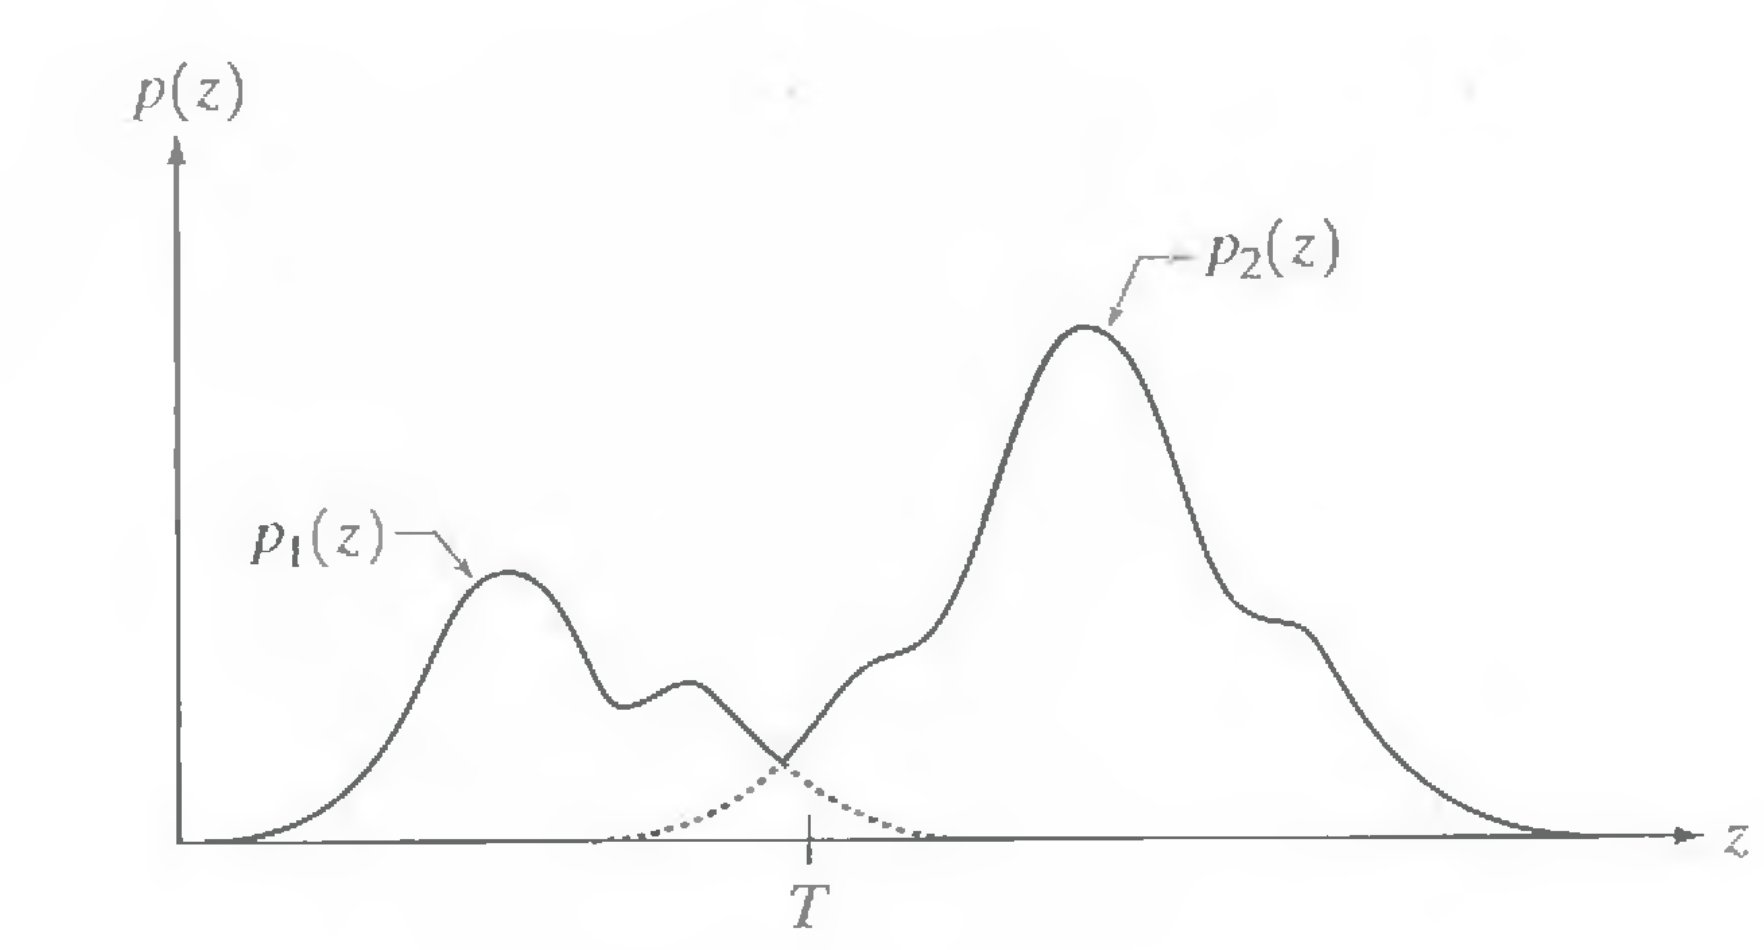
\includegraphics[width=0.8\linewidth]{bilder/Gonzalez.png}
		\caption{Histogram as a probability density function (\cite{digital_image_book})}\label{fig:gmm}
	\end{center}
\end{figure}

Probability to falsely classify an background pixel as a foreground then is:

\begin{equation}
    E_1(T) = \int_{-\infty}^T{p_2(z) \, dz}
\end{equation}

And probability to falsely classify a foreground pixel as a background then is:

\begin{equation}
    E_2(T) = \int_T^{+\infty}{p_1(z) \, dz}
\end{equation}

The overall error is:

\begin{equation}
    E(T) = P_1E_1(T) + P_2E_2(T)
\end{equation}

By differentiating $E(T)$ wrt. to $T$ and equating the result to zero the optimal solution will be:

\begin{equation}
    P_1p_1(T) = P_2p_2(T)
\end{equation}

Since Gaussian distributions have been assumed, it will hold that:
\begin{equation}
    p(z) = \frac{P_1}{\sqrt{2\pi} \sigma_1}e^{-\frac{(z-\mu_1)^2}{2\sigma_1^2}} + \frac{P_2}{\sqrt{2\pi} \sigma_2}e^{-\frac{(z-\mu_2)^2}{2\sigma_2^2}}
\end{equation}

With $\mu_i$ and $\sigma_i^2$ for $i \in \{1, 2\}$ being the mean and variance of the Gaussian distribution $p_i(z)$. This results in the following solution for $T$:
\begin{equation}
    \begin{split}
        &AT^2 + BT + C = 0 \\
        &A = \sigma_1^2 + \sigma_2^2 \\
        &B = 2(\mu_1 \sigma_1^2 - \mu_2 \sigma_2^2) \\
        &C = \sigma_1^2 \mu_2^2 - \sigma_2^2 \mu_1^2 + 2\sigma_1^2 2\sigma_2^2ln\left(\frac{\sigma_2P_1}{\sigma_1P_2}\right)
    \end{split}
\end{equation}

To escape two optimal solutions of the quadratic equation, it may be assumed that $\sigma_1 = \sigma_2 = \sigma$ and then:

\begin{equation}
    T = \frac{\mu_1 + \mu_2}{2} + \frac{\sigma^2}{\mu_1 - \mu_2}ln\left(\frac{P_2}{P_1}\right)
\end{equation}

Such threshold search is then applied to all of the subregions of the image with overlaps. Thresholds are calculated only for the regions that contain two clear peaks in their histograms and interpolated to the other pixels from the regions that do not contain them. If the subregions does not contain two peaks, it simply means that there is no foreground or background object on it. 

\begin{table}[htb]
  \centering
      \begin{tabular}{||c c||} 
       \hline
       Local Threshold & Global Threshold \\ [0.5ex] 
       \hline\hline
       0.3 sec & 17 sec  \\ 
       \hline
      \end{tabular}
      \caption{Threshold timing}
      \label{table:threshold-timing}
  \end{table}
  
Of course local thresholding approach has a longer runtime time (see Table \ref{table:threshold-timing}). Therefore when the inference speed is crutial one can still use \textit{global minimum thresholding}. It does performs visually a bit worse that a local threshold (especially for the extreme corrupted cases), however for the normal conditions the performance is quite similar ot the local thresholding (Figure \ref{fig:thresholding-bad-conditions}c).



    \subsubsection{Downstream metrics}
        In this subsection the evaluation of the model trained on full nuclei dataset with full set of augmentations is presented. Distributions of number of nuclei and their area are very similar in shape, the corresponding scatter plots form almost linear dependance. Distributions of intensities are less similar, the higher intensity of predicted images is proved here. However, high scores in Pearson and Spearman correlation coefficients (see Table \ref{table:nuclei-downstream-metrics-coefficients}) suggest that distributions are indeed close to each other. The difference between predictions and ground truth might be caused by an absolute value shift, that can be easily fixed.
\begin{figure}[htb]
	\begin{center}
		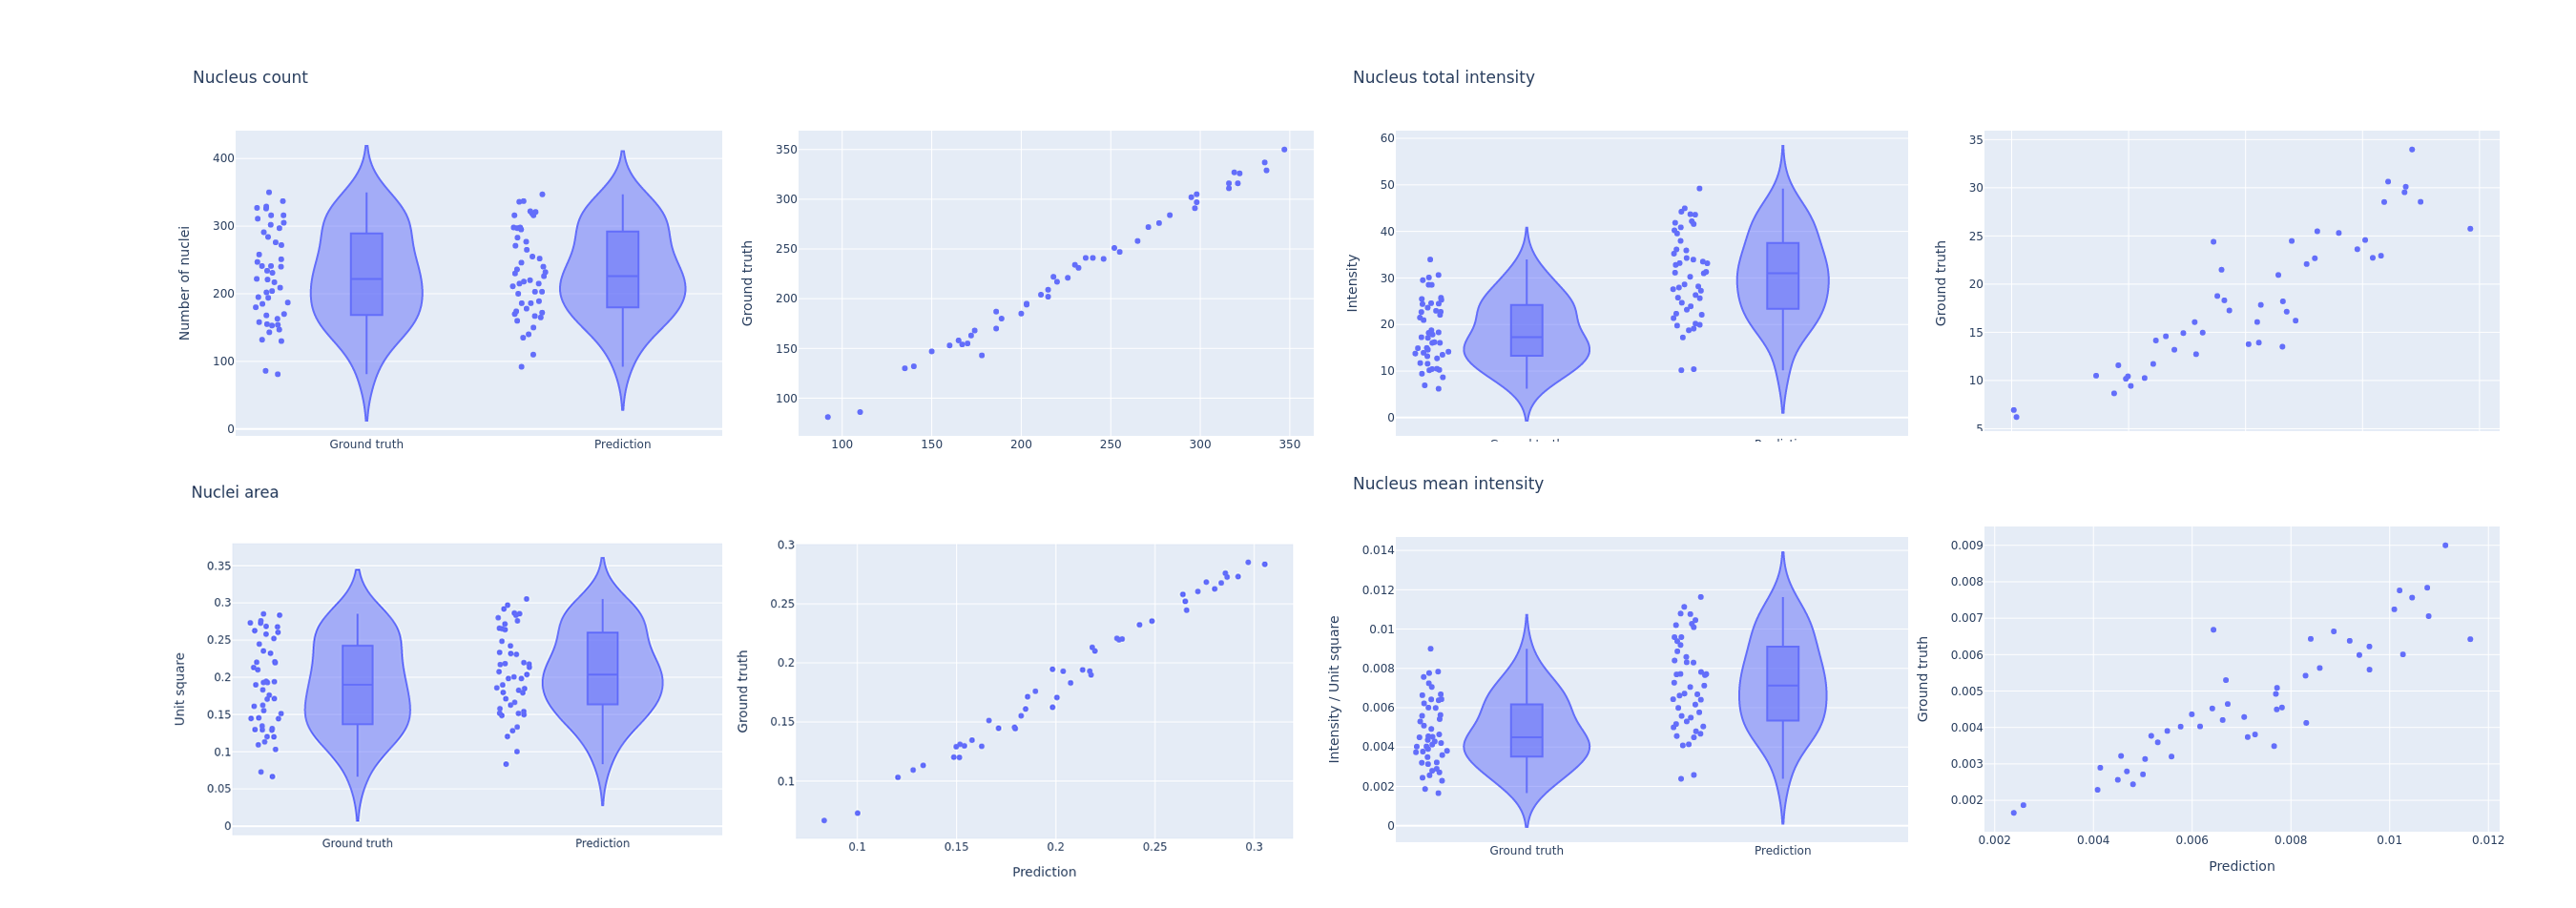
\includegraphics[width=\linewidth]{bilder/nuclei/metric/combined-metrics.png}
		\caption{Metrics for downstream tasks on nuclei}\label{fig:nuclei-downstream-metrics}
	\end{center}
\end{figure}

\begin{table}[htb]
    \centering
    \caption{Correlation coefficients for downstream tasks on nuclei}
        \begin{adjustbox}{width=0.4\textwidth}
            \begin{tabular}{|c|c|c|}\hline
                &Pearson&Spearman
                \\\hline\hline
                Number of nuclei&0.995&0.994\\\hline
                Total intensity&0.902&0.911\\\hline
                Mean intensity&0.907&0.904\\\hline
                Area&0.992&0.990\\\hline
            \end{tabular}
        \label{table:nuclei-downstream-metrics-coefficients}
        \end{adjustbox}
\end{table}

    \subsubsection{Influence of scaling on predictions quality} 
        Examples of predictions quality with different scales.

\begin{table}[H]
    \centering
    \caption{Paerson correlation coefficients for downstream tasks for different scaling factors} 
        \begin{adjustbox}{width=\textwidth}
            \begin{tabular}{|M{35mm}|M{35mm}|M{35mm}|M{35mm}|M{35mm}|M{35mm}|M{35mm}|}\hline
                &1.3 scale&0.7 scale&Train (1.0 scale + augments) \newline Predict (1.3 scale)&Train (1.3 scale) \newline Predict (1.0 scale)&Train (1.3 scale) \newline Predict (0.7 scale)
                \\\hline\hline
                Number of nuclei&0.987&0.995&0.975&0.971&?\\\hline
                Total intensity&0.902&.88&0.861&0.856&?\\\hline
                Mean intensity&0.922&0.906&0.88&0.872&?\\\hline
                Area&0.991&0.992&0.961&0.952&?\\\hline
            \end{tabular}
        \end{adjustbox}
\end{table}

    \subsubsection{Generalizability across phenotypes}
        TODO train the model on one phenotype and predict on the other, compare predictions (visually?) 
        postprocessing with metrics then?

    \subsubsection{Conclusions}
        Fluorescence staining of nucleus in CHO cells used for recombinant protein production at Merck KGaA can be successfully replaced with \textit{in silico} labeling using deep a neural network. The provided dataset is big enough to achieve accurate predictions, nevertheless further research could be dedicated to improving fluorescence image preprocessing in order to remove blur around the nucleus, as well as to cleaning the data from the under- or overexposed images.

The model successfully converges, and the use of augmentations improves its performance. Pearson correlation coefficient is more representative for the model's predictions evaluation than MSE, and MSE is not representative of a model's quality in this case. The performance of a model is evaluated in terms of practical biological metrics. Further research can also be conducted to advance the architecture of the model, as the use of more parameters improved the predictions significantly both visually and in metrics.

In order to perform segmentation of the nucleus it is recommended to use a local thresholding approach when the inference time is not crucial and global minimum thresholding algorithm when the inference time is critical. Training the model on cells of a larger size slightly improves the intensity predictions. Yet a slight change in cell size does not influence the model's performance significantly.

    \pagebreak
    \subsection{Endoplasmic Reticulum}
    Endoplasmic reticulum (ER) is a network of membranes inside a cell, through which proteins and other molecules move. Ribosomes are small and round organelles with the main function to produce the protein needed for the cell. They are located in a continuous membrane system that forms series of flattened sacs, this membrane is called ER (see Figure \ref{fig:cell}) (\cite{er}). ER itself is moslty located around the nuclei. In order to stain ER, CHO cells were treated with Donkey Anti-Rabbit IgG antibody. This is a fluorescent stain that binds strongly with ER. The analysis of this cell organelle is also important for the CLD as ER is directly related to the process of protein production within the cell: it is responsible for the synthesis, folding, modification, and transport of proteins (\cite{er_2}). The proximity of the ER to the nucleus essentially allows to control the protein production. For example, when the protein is incorrectly folded it will be accumulated in the ER lumen and it will serve as a signal to activate misfolded protein response from the cell. In contrast to other imaging datasets ER dataset does not require special preprocessing steps as the images are of a good quality and without any visible problems (see the ground truth image in Figure \ref{fig:er-combined}).
    
    \subsubsection{Training and predictions}
        During the training with PCC loss the model has successfully converged already after 35 epochs, however a clear overfit was encountered (see Figure \ref{fig:er-overfit} (left)) with the best PCC loss before the overfit being $0.0713$. Overfitting happens due to the lack of data, as for ER case there were much fewer samples than for nuclei for example (see Table \ref{table:data}). Even though one could use early-stopping approach and simply choose an earlier epoch before overfit, the better approach would be to use regularization methods described in section \ref{section:regularization}. Additional regularization in terms of data augmentations was introduced. The new learning curve is shown in Figure \ref{fig:er-overfit} (middle). Overfit happens now much later (after $120$ epochs) and PCC loss improves to $0.0701$. Introducing a stronger regularization with the use of weight decay in adadelta optimizer and dropout layers with a dropout rate of $0.1$ (see Figure \ref{fig:er-overfit} (right)) reduces the overfit completely, however at the same time increases the loss to $0.099$.
\begin{figure}[H]
	\begin{center}
		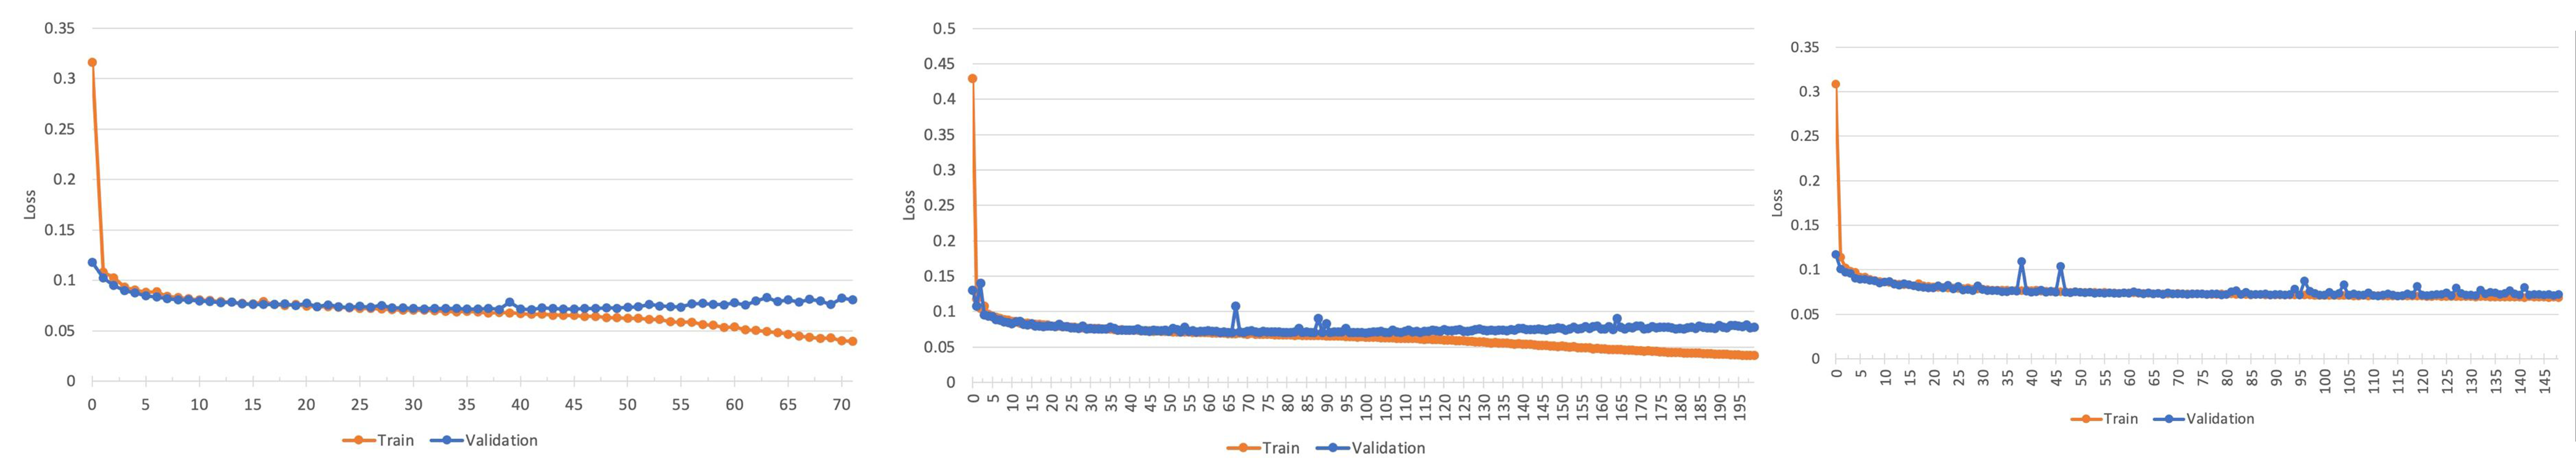
\includegraphics[width=\linewidth]{bilder/ER/segmentation/reg-not-reg.png}
		\caption{Default model (left), slightly regularized model(middle), strongly regularized model (right)}\label{fig:er-overfit}
	\end{center}
\end{figure}

Although the validation loss seem to be higher in comparison to $0.0701$, in this case the growths were not explained by the difference between the validation sets, where the loss was measured on. PCC losses on the same validation set for both were $0.0701$ and $0.0742$. It might have been the case that the regularization was too strong. In this case it would be better to use early-stopping approach with the epoch that has the lowest loss.
    \subsubsection{Combination of nuclei and actin predictions}
        Now having two models for the predictions of two organelles: nuclei and ER, it is interesting to visualize the predictions together (see Figure \ref{fig:er-combined}). It is clear from the image that ER indeed is located around the nucleus. As one can see, there is a great advantage in the used of \textit{in silico} fluroescence labeling especially for the cases where several cell targets have to be ananlysed. Instead of a expesive and time-consuming procedure for staining several targets at the same time they can be predicted based on one DIC image only.
\begin{figure}[htb]
    \centering
    \setkeys{Gin}{width=\linewidth}
    \centering
        \begin{tabularx}{\textwidth}{YYYY}
            (a)  \textbf{Ground truth} &
            (b)  \textbf{Prediction} &
            (c)  \textbf{Prediction + nuclei} \\
            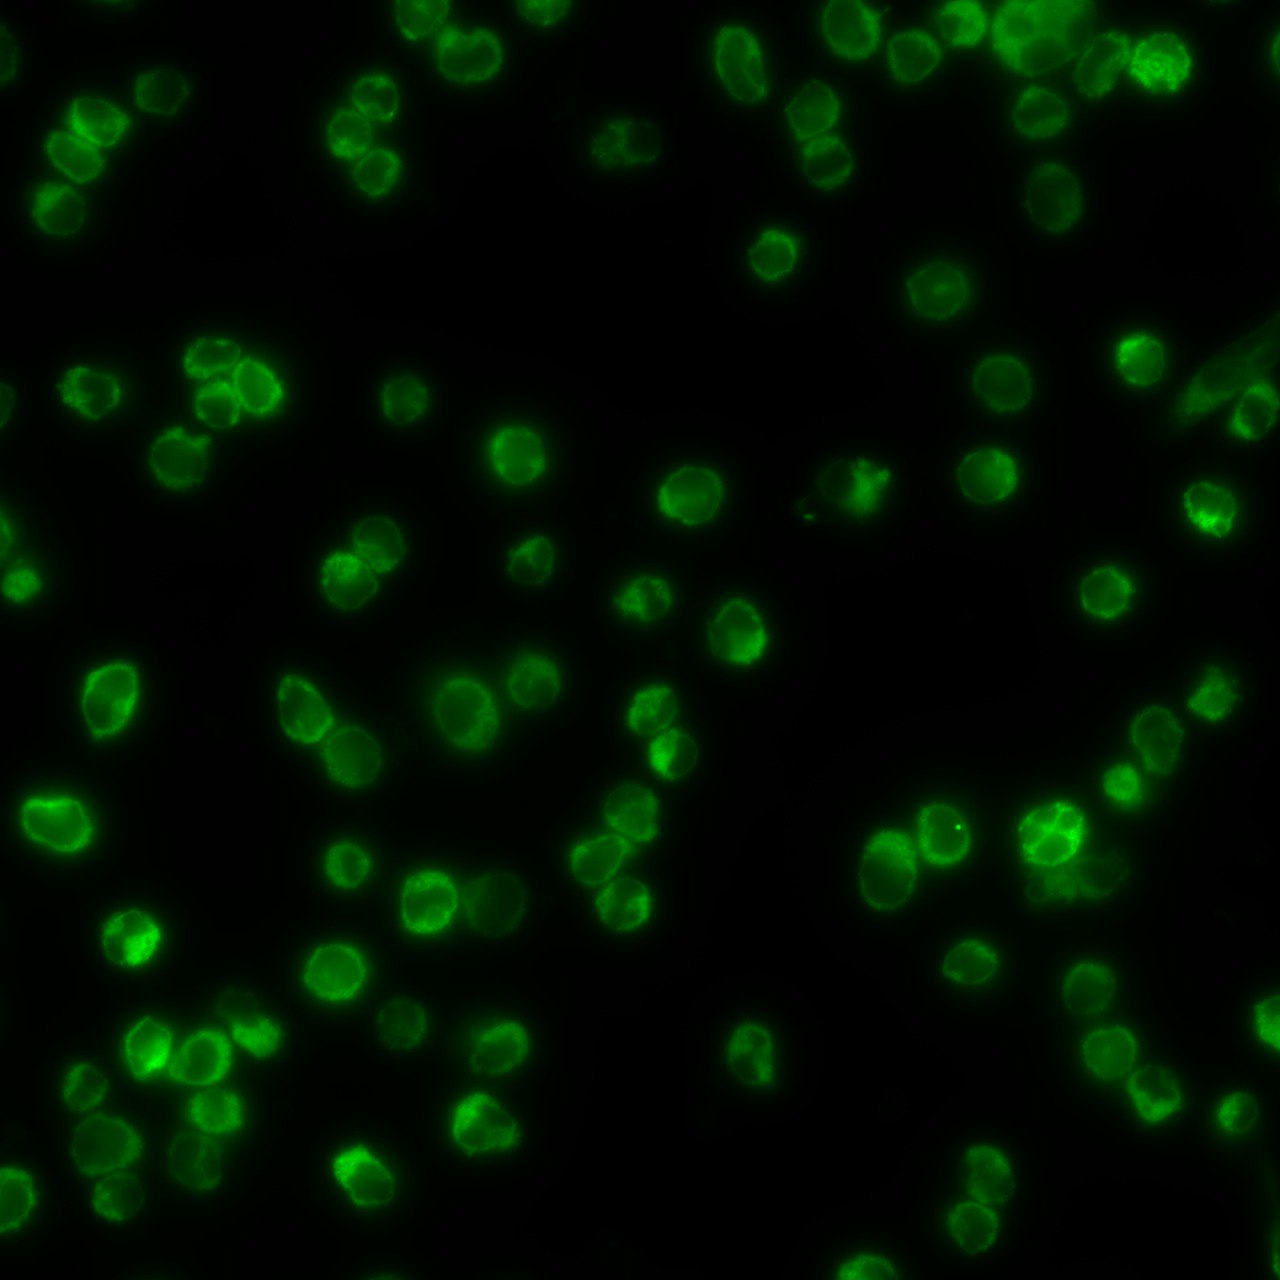
\includegraphics{bilder/ER/gt.jpg} & 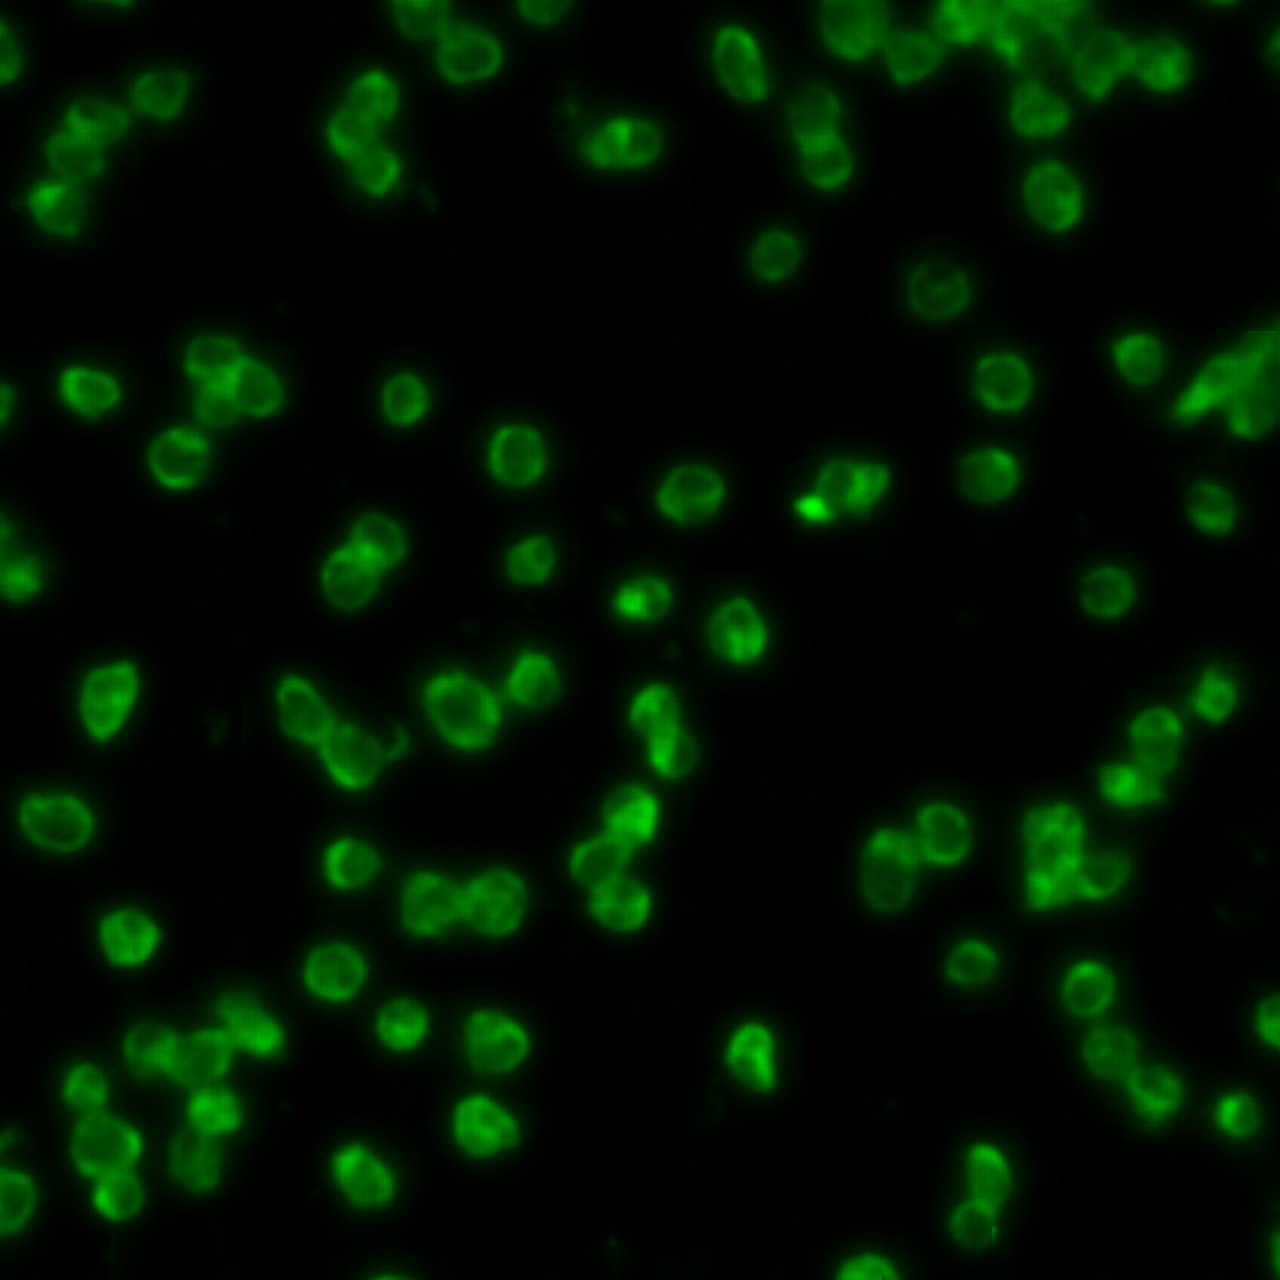
\includegraphics{bilder/ER/er.jpg} &
            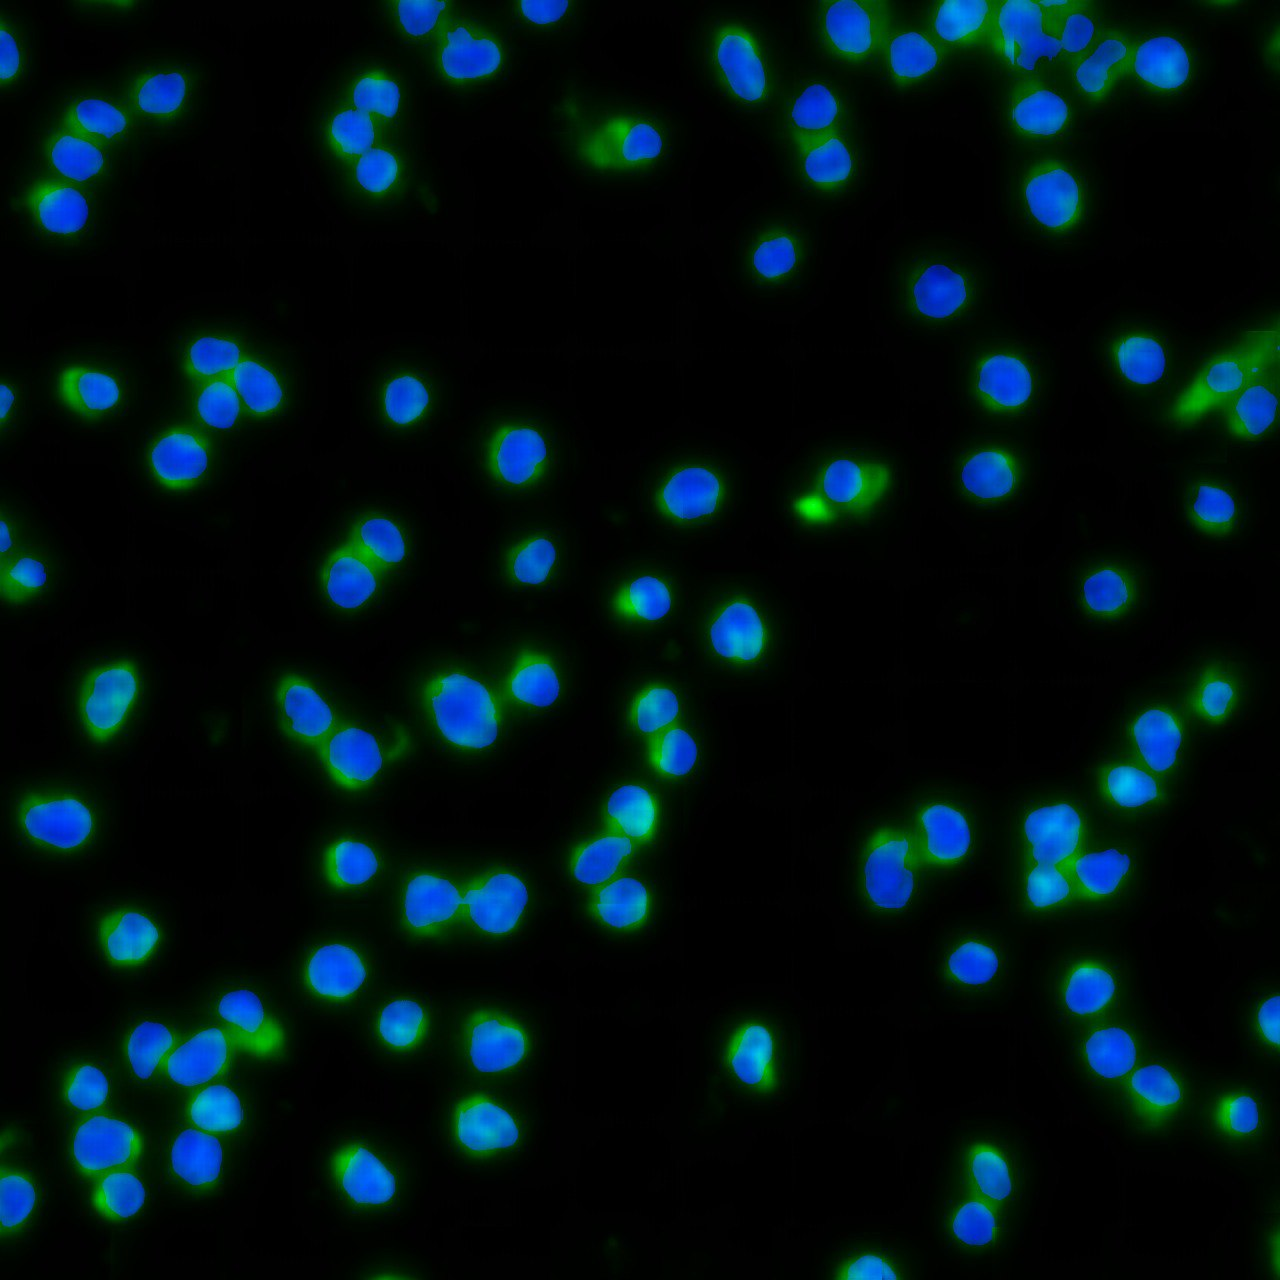
\includegraphics{bilder/ER/gt_nuclei.jpg}
        \end{tabularx}
    \caption{Combination of ER with nuclei prediction. Image (a) here is the original fluorescence image of ER, image (b) is the UNet prediction of ER and image (c) is the combination of predicted ER (green) with predicted nuclei (blue).}
    \label{fig:er-combined}
\end{figure}
    \subsubsection{Postprocessing for ER segmentation}
        The process of ER fluorescence segmentation is somewhat different in comparison to nuclei segmentation. These fluorescence staining has a stronger "shining" around the ER itself and therefore any method for background removal would be helpful to reduce it. One of such methods based on the rolling ball algorithm is described in more details in section \ref{par:background-removal}.

Initially it was established that a local thresholding approach for segmentation would be nessecary here as well, as the images also have a non-uniform illumitation. However a downside of a local thresholding algorithm is the appearance of the artifacts briefly mentioned in the previous section and presented in Figure \ref{fig:artifacts-er}. Even though the background in fluorescence imaging appears to be completely black, it still contains some slight signal (non-zero values), that are boosted by a local threshold and becomes an unwanted artifact. 
\begin{figure}[H]
	\begin{center}
		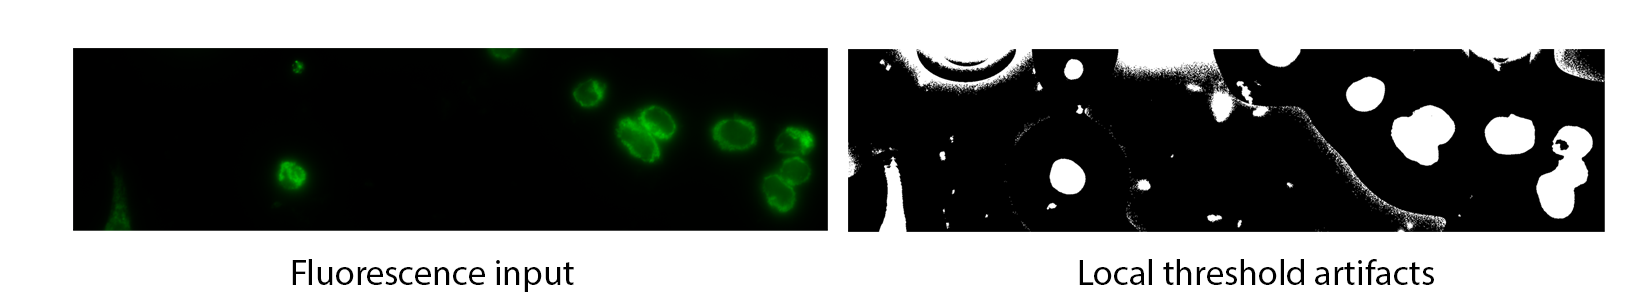
\includegraphics[width=\linewidth]{bilder/ER/artifacts.png}
		\caption{Artifacts from local thresholding algorithm}\label{fig:artifacts-er}
	\end{center}
\end{figure}
Such falsely recognized regions appeared in the nuclei as well, yet there they were easily filtered out based on the shape criteria. All nuclei are almost round and convex objects, whereas background artifacts are prolonged completely non-convex objects. Unfortunately, such filtration cannot be applied to ER imaging as very often ER from one cell is located very close one to the ER from another cell, and together they may form a long non-convex object, that now could not be filtered out this easily. That is why it is very important to remove the background noise here first before applying a local threshold.

In order to do that one can first apply a rough "over-predictive" global thresholding, that will cover a true signal fully, including the "shine" around the ER, but will ignore the background noise. In the role of "over-predictove" global mean thresholding algorithm can be used (see Figure \ref{fig:er-segmentation-steps}.2). The mask created with the mean thresholding approach is used to zero out all the pixels that are not covered by it. And after that the local thresholding can be successfully applied with the \textit{block\_size} of $181$ (Figure \ref{fig:er-segmentation-steps}.4). Then  algorithm fills in all the holes in the middle of ER that might have appeared during the thresholding. Morphological opening (see Section TODO cite section) and Gaussian Blur with the squared kernel $3 \times 3$ are applied. Connected components are detected afterwards and filtered based on the limit of the area they occupy, this filters out mostly very small components from the mask which might be produced by the left out background noise. The whole algorithm overview is described below:

Segmentation steps are described in Algorithm \ref{alg:er-segmentation-steps} and also illustrated in Figure \ref{fig:er-segmentation-steps}.

\begin{algorithm}
    \caption{Fluorescence segmentation}
    \begin{algorithmic}
    \item 1. Normalize image
    \item 2. Apply global \textit{threshold\_mean} to receive initial mask.
    \item 3. Zero out pixels outside the mask
    \item 4. Apply local thresholding.  
    \item 5. Apply \textit{fill\_holes} transformation.
    \item 6. Morphological opening from OpenCV and Gaussian blur.
    \item 7. Run \textit{findContours} from OpenCV in order to obtain separate regions and filter out too small regions.
    \end{algorithmic}
    \label{alg:er-segmentation-steps}
\end{algorithm}    

\begin{figure}[htb]
    \begin{center}
        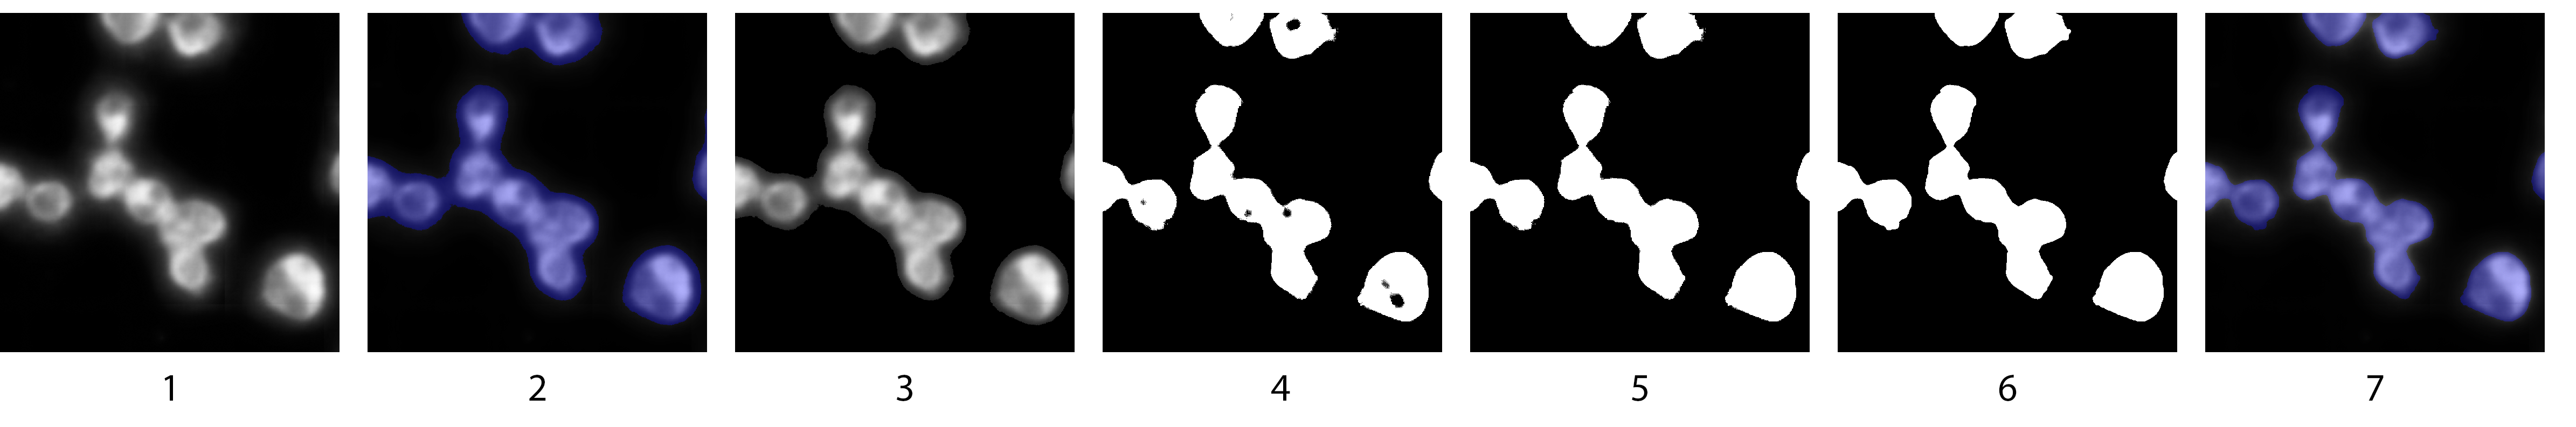
\includegraphics[width=\linewidth]{bilder/ER/segmentation/segmentation.png}
        \caption{Segmentation steps in ER postprocessing}\label{fig:er-segmentation-steps}
    \end{center}
\end{figure}
    \subsubsection{Conclusions}
        Training the model on the ER stain images produced very successful results that can be used as a replacement for manual staining with \textit{in silico} labeling. Overfit of the model has been encountered and several experiments were performed to overcome it, the best checkpoint was selected and evaluated.

The segmentation of ER for further downstream metrics evaluation was proposed. The problem of overlap between cells being present was discovered, which causes the segmented regions to merge together. Subsequently, a better preprocessing algorithm was proposed. This algorithm helps to avoid the artifacts appearing from a local thresholding.

The combination of ER with nuclei predictions was visualized and analysed, it was confirmed that the models produce realistic results confirming biological definition of their mutual arrangement within the cell. However, it is recommended to test the models using the simultaneous staining of both organelles to get quantitative metrics of the accuracy.
    \subsubsection{Generalizability across phenotypes}
        TODO move into the other section, there is only 1 phenotype here
        TODO train the model on one phenotype and predict on the other, compare predictions (visually?) 
        postprocessing with metrics then?
        Add metrics

    
    \pagebreak
    \subsection{Golgi}
    \subsubsection{Preprocessing}
        Enhancement
        One can see an example of how Golgi fluorescence staining looks like in Figure \ref{fig:golgi-enhancement}. It is evident that there is a lighter foreground fluorescence and a bit darker one in the background. A true Golgi signal here is considered to be only the lighter part of fluorescence lightning. The light gray background present here is called a non-specific fluorescence lightning. It comes from the cell itself, and might occur when the antigen is impure and contains antigenic contaminants (\cite{Borek_1984}). And brightness of it may vary due to longer or shorter exposure times. 

\begin{figure}[htb]
	\begin{center}
		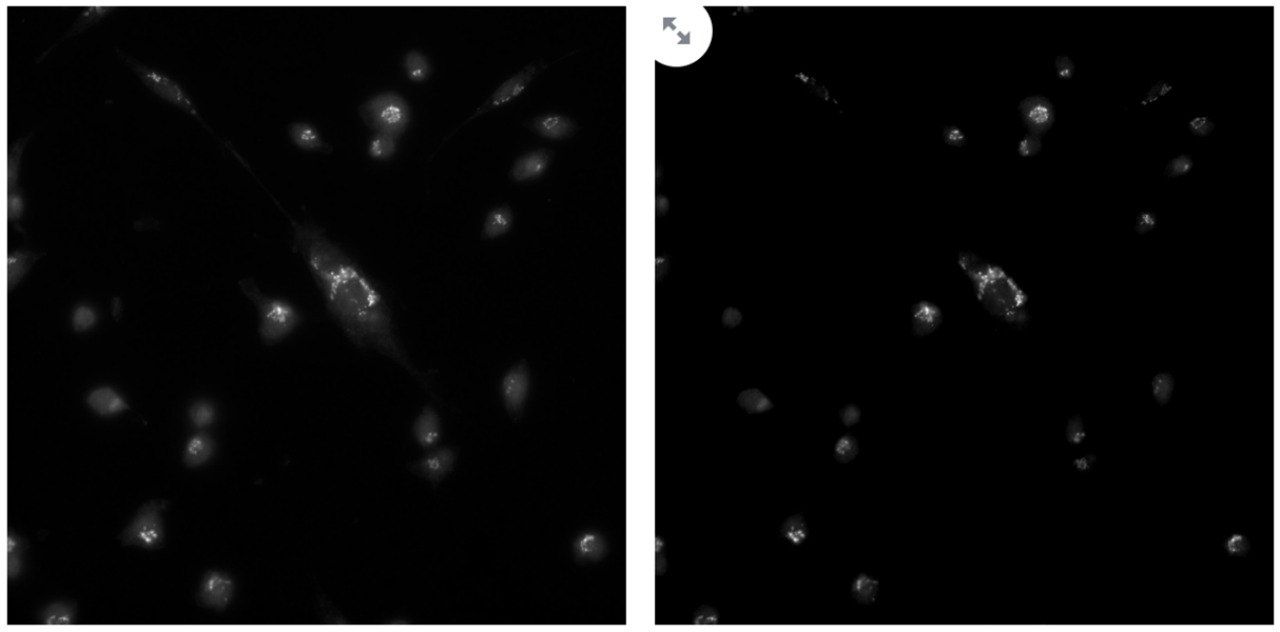
\includegraphics[width=0.5\linewidth]{bilder/enhancement.jpg}
		\caption{Golgi enhancement: left --- original signal, right --- enhanced image}\label{fig:golgi-enhancement}
	\end{center}
\end{figure}

Having such a non-specific fluorescence background has two challenges for training:
\begin{itemize}
    \item The relative area of the background fluorescence is bigger than the area of Golgi themselves. Therefore quite a big part in the loss during training will be dedicated to teaching model to restore this background fluorescence instead of the Golgi itself.
    \item It introduces difficulties during the post-processing of the predictions. As well as for nuclei, the mask of the predicted Golgi apparatus is needed for further evaluation of the downstream metrics. Using the same algorithm for post-processing segmentation that was used for nuclei, the mask of the Golgi Apparatus will consider the background noise to be relevant, although this is an unwanted behavior.
\end{itemize}

On the left of Figure \ref{fig:golgi-enhancement} one can see the original ground truth image and on the right --- the images after the background was substracted. One of the great background subtraction algorithms is the rolling ball algorithm which is described below.

Additionally, all of the crops used for training were filtered base on the amount of background they contain. Without filtering the crops that contain a lot of background, a big portion of a dataset would be black crops only, which creates very strong class imbalance.

        \paragraph{Background removal algorithms}
            The rolling ball algorithm was introduced by \cite{Sternberg_1983} and is still widely used for processing medical and biological data. The idea of this algorithm is based on morphological opening of the image. 

\begin{definition}[Morphological opening]
	Morphological opening is an operation in image processing, when an image is first eroded and then dilated using the same structuring element. 
\end{definition}

Morphological opening is helpful for removing noisy elements, thin lines, while preserving bigger objects in the image (\cite{morph_open}).

A structuring element is an analog of a kernel in image processing. It is a matrix of zeros and ones (true and false), where ones represent the elements that will be used to perform the morphological operation and others will be ignored (see an example in Figure \ref{fig:rolling-ball} [left]). Such a structuring element is applied across the whole input image producing a new image based on the rules of a morphological operation it performs.  

For example, morphological dilation takes a new value of the pixel as the maximum value of its neighbors within the structuring element. Therefore, after this operation, the lines will be thicker and in general objects will appear bigger.

Whereas morphological erosion turns the pixel value into the minimum value of its neighbors within the structuring element. After this operation the floating pixels will be removed and all objects become smaller and thinner.

\cite{Sternberg_1983} has extrapolated the operation of morphological opening from 2D into 3D space. He defines a new interpretation of a 2D image in a 3D world called umbra. Umbra can be described as a 3D plane, where the height of each point is determined by its intesity value.

The structuring element for morphological opening of an umbra has to be then also a 3D object --- in this case a ball. Morphological opening of an umbra is a union of translations of the 3D structuring element that can be entirely contained inside it (see Figure \ref{fig:rolling-ball}). One can imagine the ball freely moving inside the volume constrained by the upper surface of an umbra. The opening then consists of all the pixels that can be reached by the ball. The radius of the ball is a hyper-parameter which has to be tuned.

\begin{figure}[H]
    \centering
    \subfloat[Structuring element]{{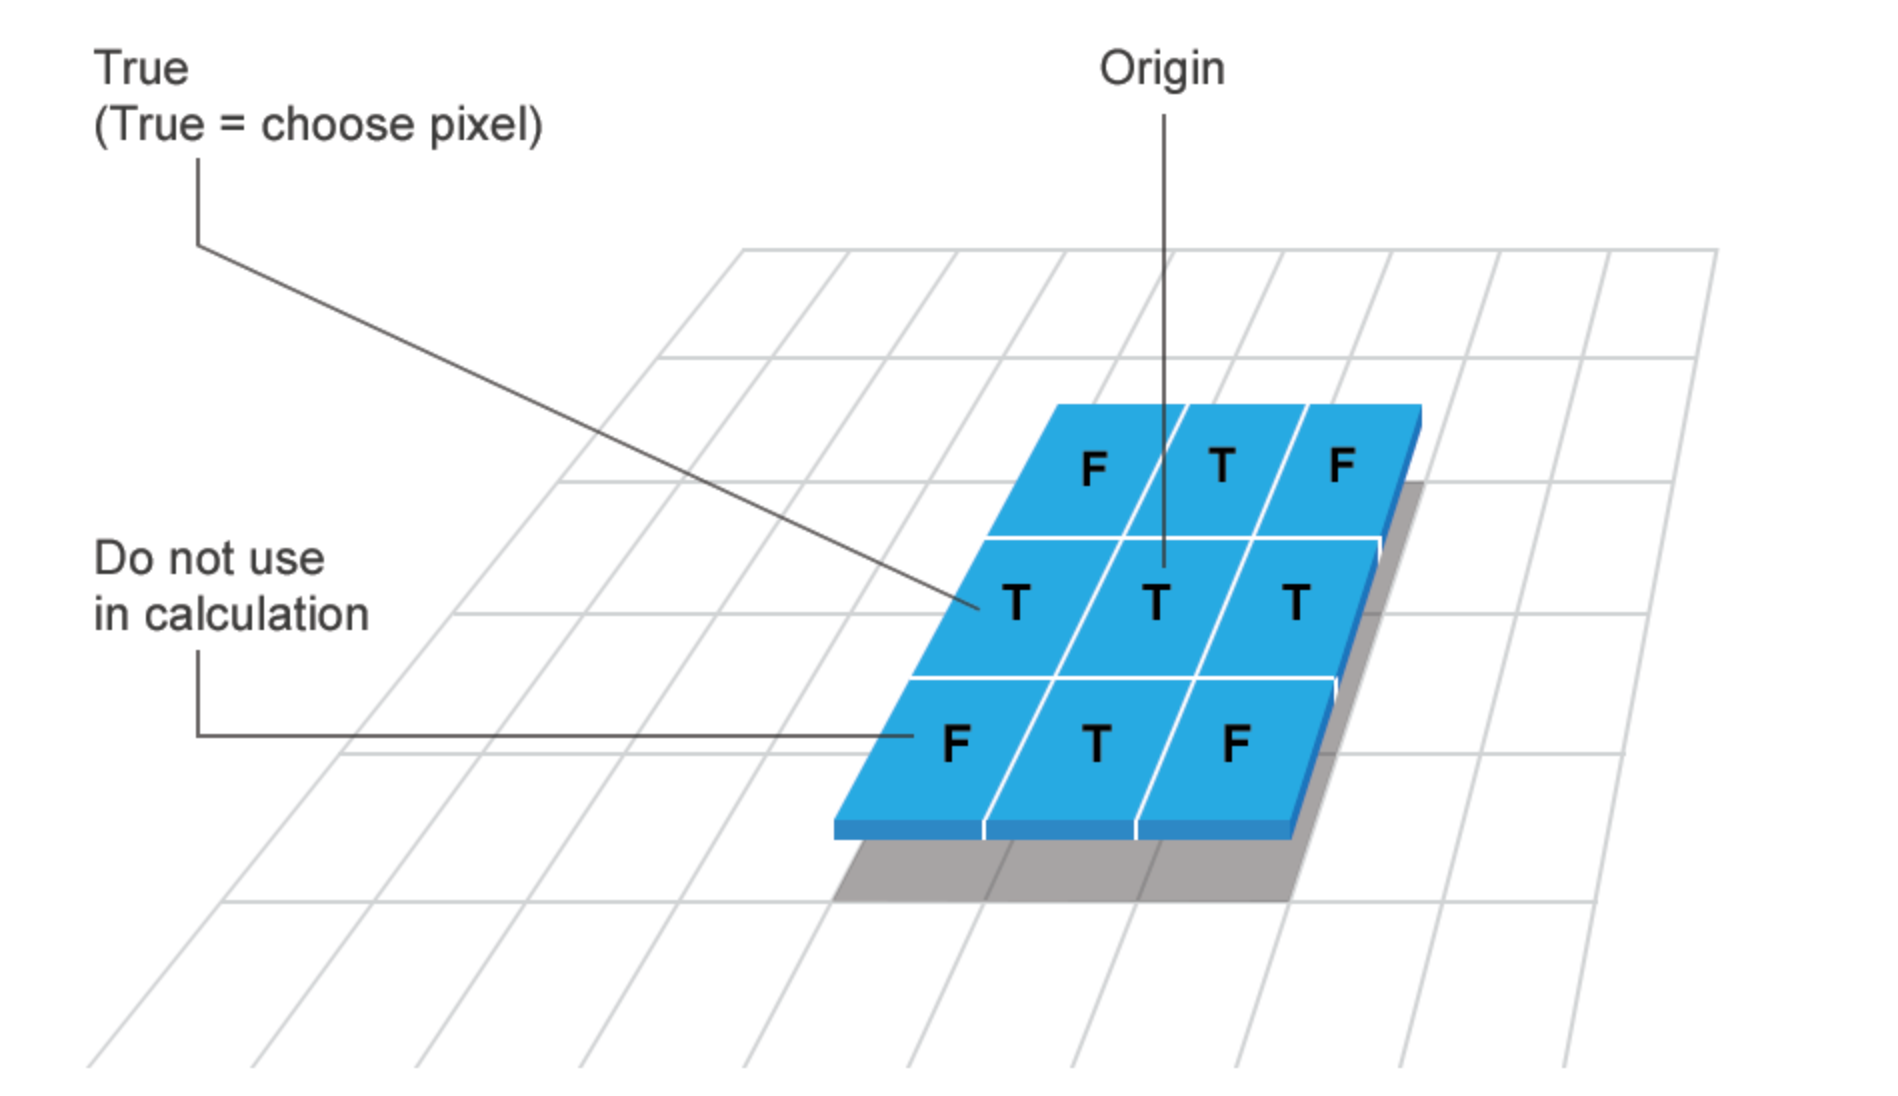
\includegraphics[width=0.3\linewidth]{bilder/structuring-element.png} }}
    \qquad
    \subfloat[Rolling ball]{{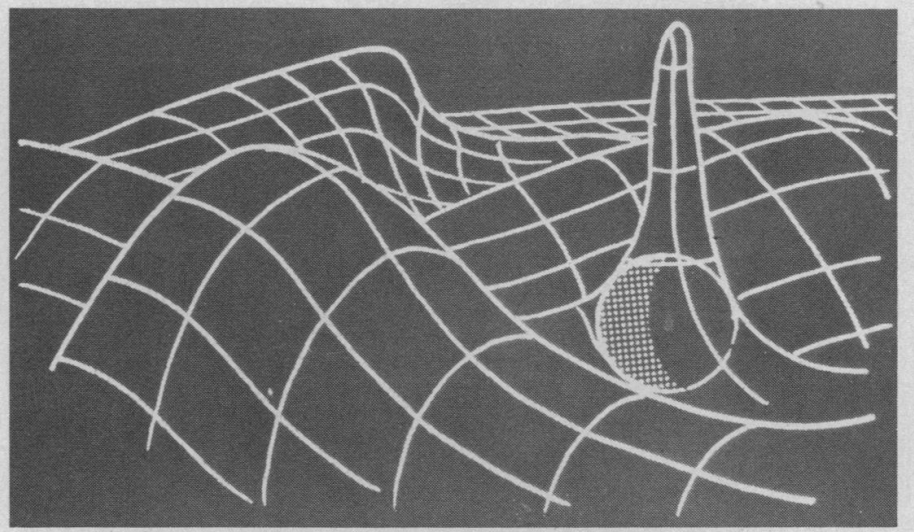
\includegraphics[width=0.3\linewidth]{bilder/rolling-ball.png} }}
    \caption{Background removal}
    \label{fig:rolling-ball}
\end{figure}

Subtracting the background with the rolling ball algorithm unfortunately is still not enough to get a reasonably clean signal of Golgi apparatus from fluorescence imaging, as a lot of background noise will still be present there. In Figure \ref{subfig:vanilla} one can see a fluorescence image preprocessed with a rolling ball algorithm. Let's turn it into a binary image that can be seen in Figure \ref{subfig:vanilla-mask}. 
\begin{figure}[htb]
	\centering
	\begin{subfigure}[b]{0.22\textwidth}
		\centering
		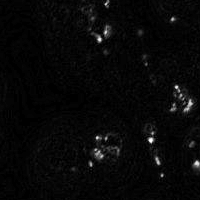
\includegraphics[width=\textwidth]{bilder/preprocessing/crop_golgi_not_full_processed.png}
		\caption{}
		\label{subfig:vanilla}
	\end{subfigure}
	\hfill
	\begin{subfigure}[b]{0.22\textwidth}
		\centering
		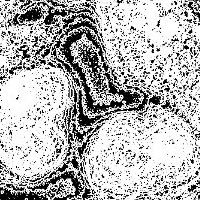
\includegraphics[width=\textwidth]{bilder/preprocessing/crop_golgi_not_full_processed_mask.png}
		\caption{}
		\label{subfig:vanilla-mask}
	\end{subfigure}
	\hfill
	\begin{subfigure}[b]{0.22\textwidth}
		\centering
		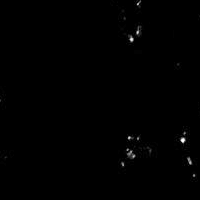
\includegraphics[width=\textwidth]{bilder/preprocessing/crop_golgi_full_processed.png}
		\caption{}
		\label{subfig:clipping}
	\end{subfigure}
	\hfill
	\begin{subfigure}[b]{0.22\textwidth}
		\centering
		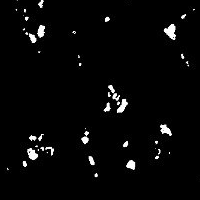
\includegraphics[width=\textwidth]{bilder/preprocessing/crop_golgi_full_processed_mask.png}
		\caption{}
		\label{subfig:clipping-mask}
	\end{subfigure}
	   \caption{(a) Vanilla preprocessing with automatic background removal algorithm only; (b) masked or subfigure (a); (c) Additional clipping of lower intensities after vanilla pre-processing; (d) mask of subfigure (c)}
	   \label{fig:pre-processing-golgi}
\end{figure}
It clearly still contains a lot of background noise of low intensity which was not visible for an eye. In order to get rid of it one could clip lower intensities of the image via the following approach:
\begin{lstlisting}
	import numpy as np
		
	def clip(image):
		minval = np.percentile(image, 90)
		image = np.clip(image, minval, image.max())
		image = (image - image.min()) / (image.max() - image.min())
		return image
\end{lstlisting}

The result of the clipped image and its mask are illustated in Figure \ref{subfig:clipping}, \ref{subfig:clipping-mask} correspondingly. It contains almost no background noise now. Such additional clipping might improve the results slightly.
    \subsubsection{Training and predictions}
        Applying the usual model architecture with PCC loss too train the model to predict fluorescence signal from DIC imaging for Golgi did not bring a good results. Model seems to converge (see Figure \ref{fig:golgi-no-reg-pcc}), however there is no learning happening.
\begin{figure}[H]
	\begin{center}
		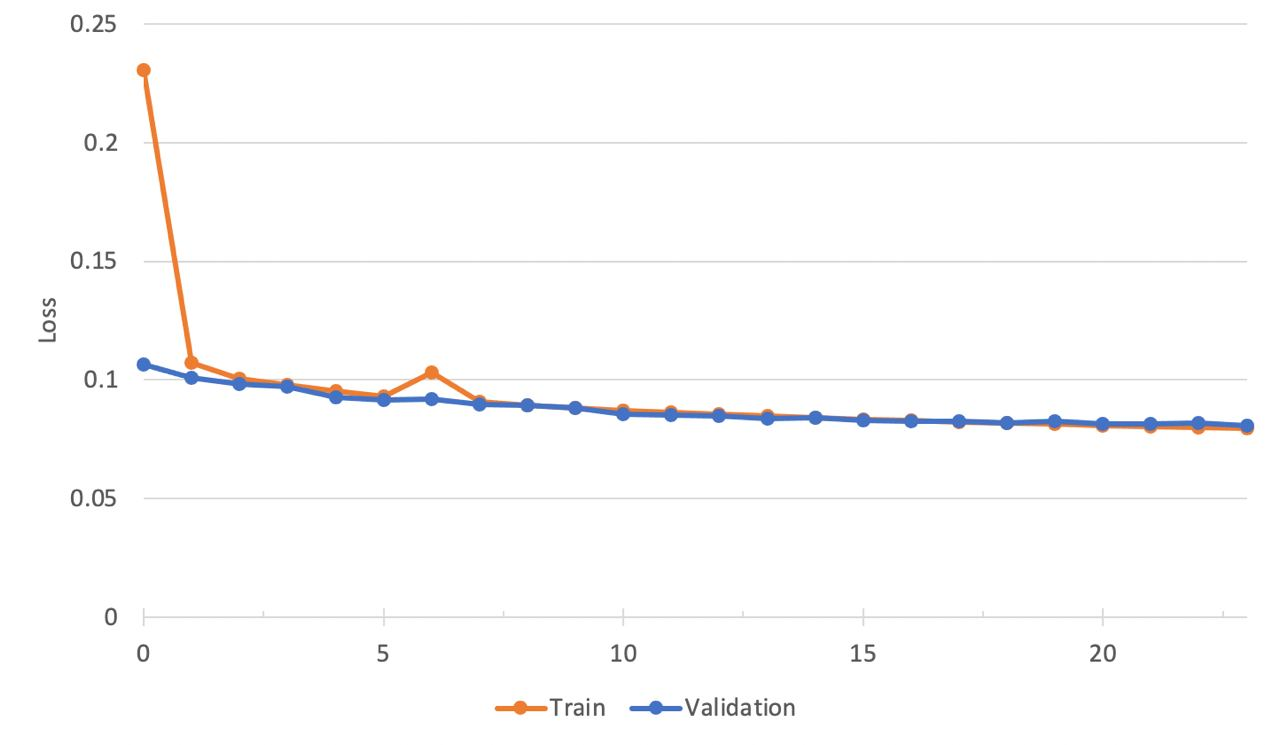
\includegraphics[width=0.8\linewidth]{bilder/golgi/pcc-no-reg.jpg}
		\caption{Straightforward training doesn't work}\label{fig:golgi-no-reg-pcc}
	\end{center}
\end{figure}

This was also depicted in visual predictions where the predicted fluroescence mostly contains dark pixels only (see Figure \ref{fig:golgi-no-reg-pcc-predictions}). Altough it seems that some pattern is hidden behind the dark pixels, visualizing it simply shows that the model picks up on the cell outline itself and does not give any useful information on the location of Golgi. One can see this by normalizing the predicted dark image to the range $[0,1]$ (Figure \ref{fig:golgi-no-reg-pcc-predictions}).
\begin{figure}[htb]
	\begin{center}
		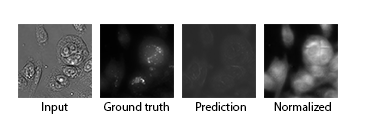
\includegraphics[width=0.8\linewidth]{bilder/golgi/too-dark.png}
		\caption{Training on original data}\label{fig:golgi-no-reg-pcc-predictions}
	\end{center}
\end{figure}

While in Figure \ref{fig:golgi-no-reg-pcc-predictions} only the results of predictions for one crop are presented, it would be interesting to see how the image with combines crops would look like. This is presented in Figure \ref{fig:golgi-no-reg-pcc-predictions-full}. One can notice an interesting pattern there: essentially the model is predicting some signal across the whole cell with a brighter regions in some of them. Yet these regions do not have a correct location wrt to Golgi. Also it is important to keep in mind, that the image of the right in this Figure is a normalized one and a true image is almost fully black.
\begin{figure}[htb]
	\begin{center}
		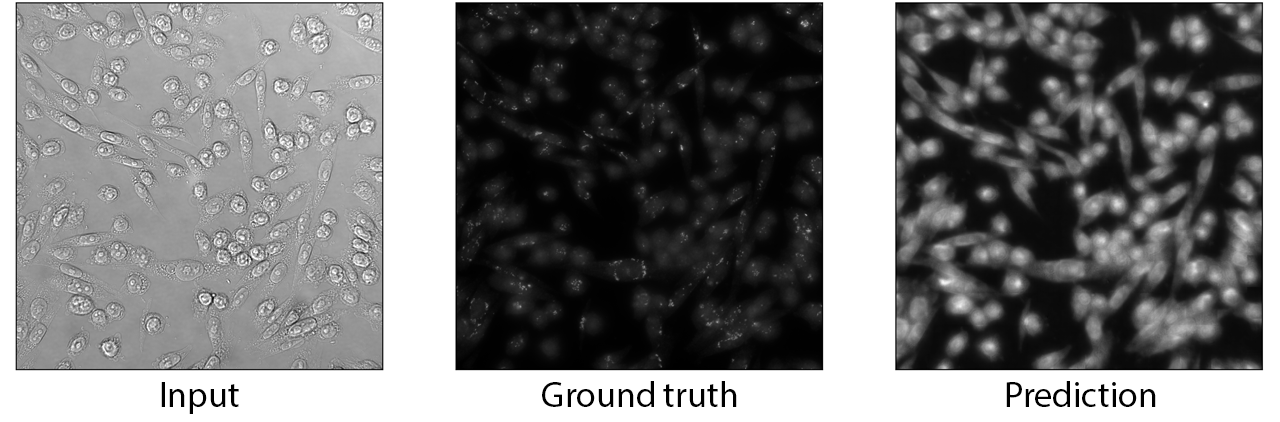
\includegraphics[width=0.8\linewidth]{bilder/golgi/full-img.png}
		\caption{Full size predictions}\label{fig:golgi-no-reg-pcc-predictions-full}
	\end{center}
\end{figure}

This experiment brought a hypothesis that the background removal algorithm might have reduces the signal-to-noise ratio and remove some important fluroescence signal along the way. Therefore an alternative approach of a background removal had been tried, where only enhancing via clipping described above has been applied directly on fluprescence imaging (without using a rolling ball algorithm). This produces images that still have much more non-specific fluorescence background (see Figure \ref{fig:golgi-enhanced-predictions} (second image)), yet this preprocessing alternates the initial image to a much lower extent.

\begin{figure}[htb]
	\begin{center}
		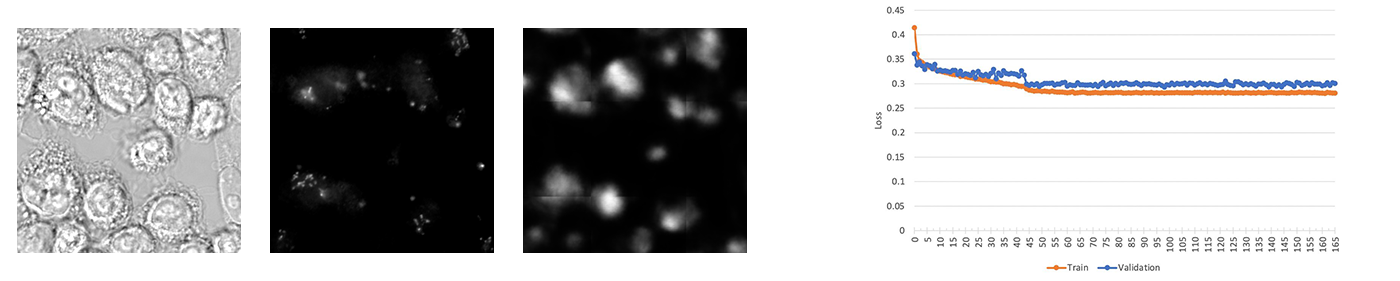
\includegraphics[width=\linewidth]{bilder/golgi/enhanced-crop.png}
		\caption{Training on the enhanced data}\label{fig:golgi-enhanced-predictions}
	\end{center}
\end{figure}
In this case predictions are not completely black anymore, however their quality is still very low. Images used in these training experiments were effectively coming from different staining procedures, using different antibodies, fixation process and microscopy settings. This brought up an idea to train the model on few selective datasets only that were created with the first staining approach only. The preprocessing was chosen as in the previous example --- with the use of enhancement and without rolling ball algorithm as it has shown the best results.

\begin{figure}[htb]
	\begin{center}
		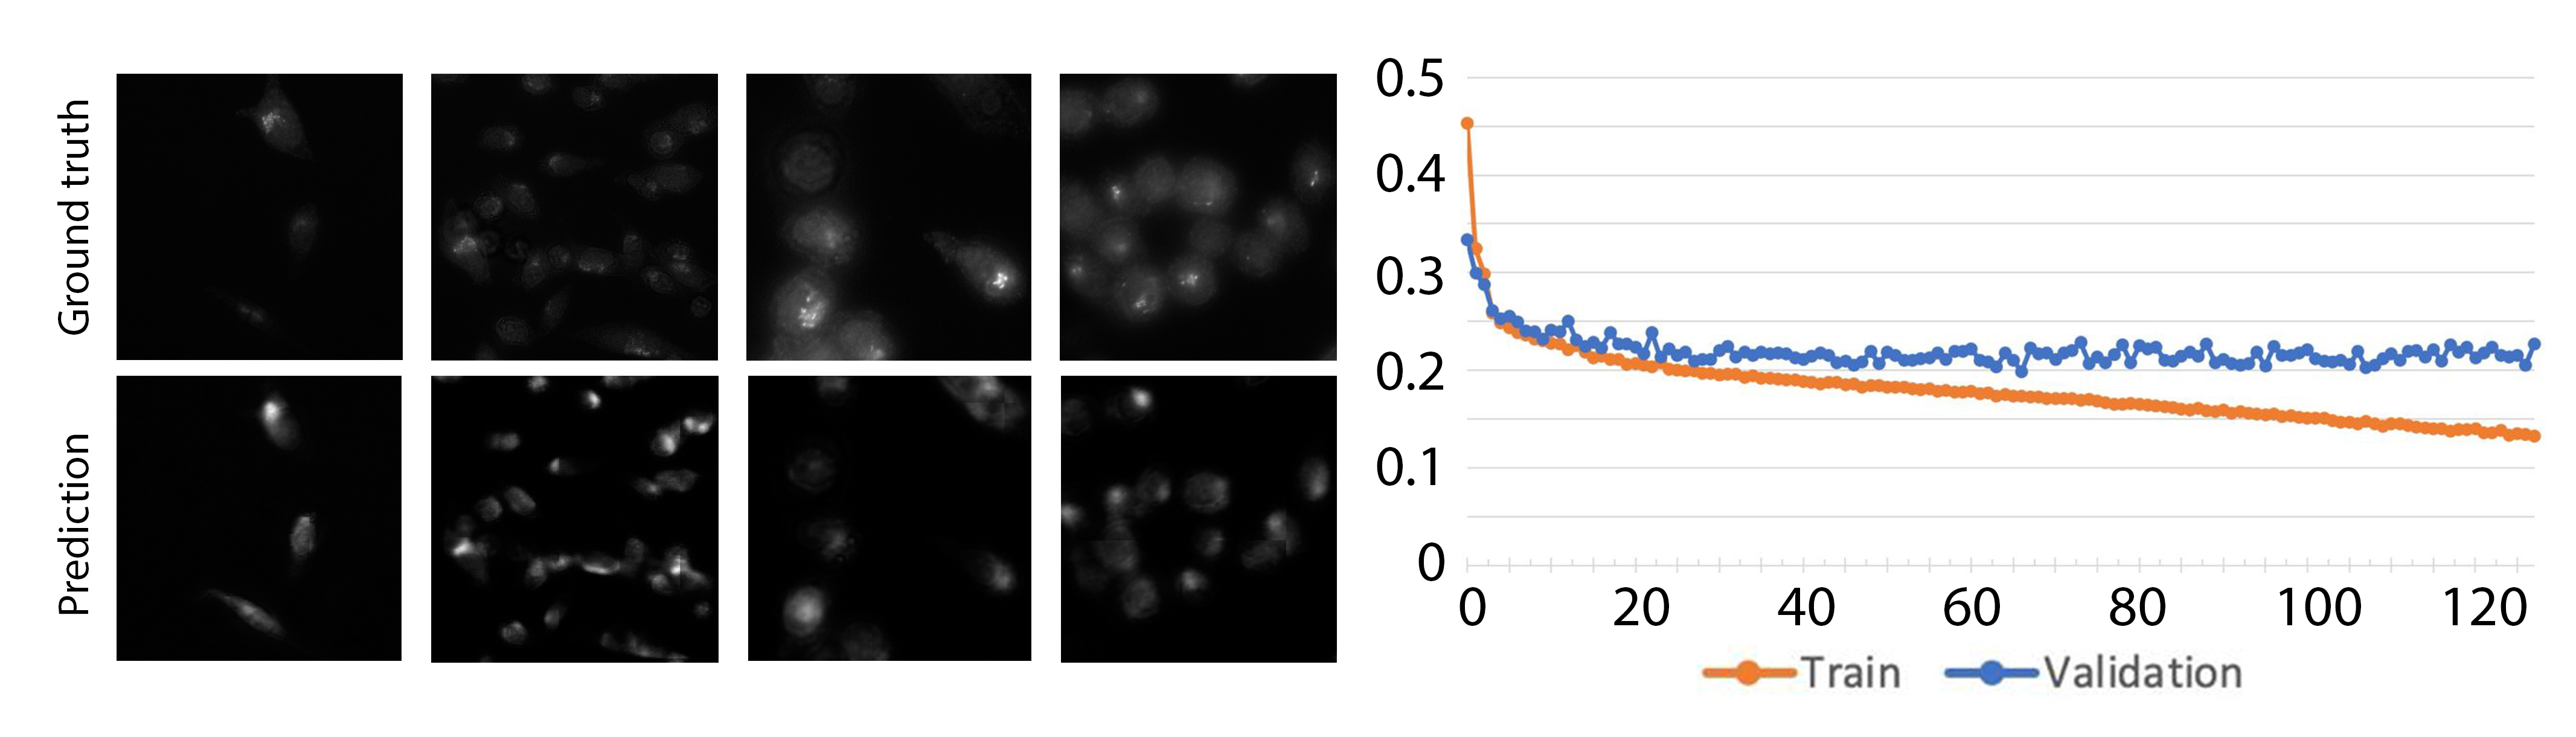
\includegraphics[width=\linewidth]{bilder/golgi/12-13/12-13.png}
		\caption{Small subset of the best staining}\label{fig:12-13}
	\end{center}
\end{figure}

The predictions from this experiment you can find in Figure \ref{fig:12-13}. Due to the stricter filtering and the use of much less data there were much smaller crops which were used for training. In this case only $4251$ crops were used for training and $406$ for validation purposes, which directly led to overfitting after $70$ epochs. However, the predictions did improve visually as well as the loss dropped to $0.19$. Nevertheless the losses from these two experiments should not be compared directly as they were evaluated on two different validation sets. The improvement of the results indicated the careful choice of data samples taken from the same staining approach with the same settings, that does not require a severe preprocessing and already has a high signal-to-noise ratio might help the predictions significantly. There is a potential here for a better regularization of the model trained on the small subset of data. Yet it is clear that the acquisition of a better fluorescence staining is much more crucial here.


    \subsubsection{Alternative ways to improve predictions}
        \paragraph{Asymmetrical losses}
            The earliest learnings from the experiments have shown that the severe class imbalance is present and the model tends to predict mostly pure background --- black images. In order to overcome this an asymmetrical loss can be used during training. Similarly to a weighted loss for a classification problem with class imbalance issue present, a weighted loss for segmentation task can be introduced. In this case different pixels from the prediction will receive a different weight based on some criteria. Yet the use of weights cannot be easily defined for Pearson correlation coefficients, it is possible to use them with MSE loss, because weights coefficients there can be added directly in front of the squared difference between pixels. 
\begin{figure}[H]
	\begin{center}
		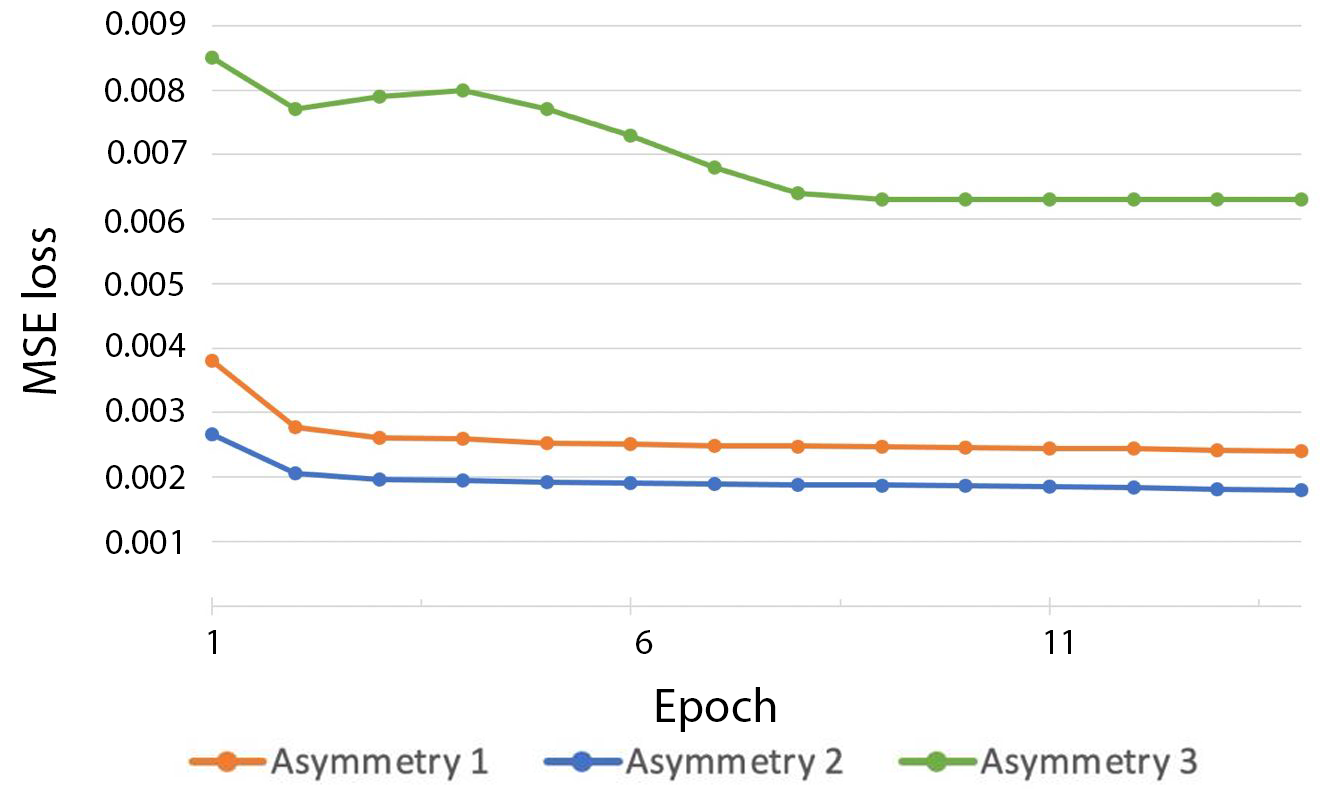
\includegraphics[width=0.5\linewidth]{bilder/golgi/asymmetrical-training.png}
		\caption{Punishing over and under predictions with asymmetrical MSE loss}\label{fig:golgi-asymmetrical-training}
	\end{center}
\end{figure}

Figure \ref{fig:golgi-asymmetrical-training} presents training learning curves from three asymmetrical approaches.

Asymmetry 2 is aimed to punish the errors on bright pixels more: when a model's pixel prediction is higher than a true one the loss will be higher. Yet this loss also encourages the model to underpredict and results in completely black images even though it has the lowest loss.
  \begin{lstlisting}
	  residual = prediction - ground_truth
	  loss = torch.where(residual < 0, residual ** 2, 2 * (residual) ** 2)
	  loss = torch.mean(loss)
	\end{lstlisting}

Asymmetry 1 is aimed to do the opposite and punish an underprediction: when a model's pixel prediction is lower than a true one the loss will be higher. This resulted in slightly brighter images
\begin{lstlisting}
	residual = prediction - ground_truth
	loss = torch.where(residual > 0, residual ** 2, 2 * (residual) ** 2)
	loss = torch.mean(loss)
  \end{lstlisting}

Asymmetry 3 is a stronger version of Asymmetry 1 and it results in 
	\begin{lstlisting}
		residual = prediction - ground_truth
		loss = torch.where(residual > 0, residual ** 3, 20 * (residual) ** 2)
		loss = torch.mean(loss)
	  \end{lstlisting}

All of the approaches above do not bring a significant change in the performance and a mostly black image remained to be an output. Interestingly, punishing underprediction has essentially backfired, as loss then supports an overprediction. Because setting the weights of one class to be smaller amounts to the same as setting the weights of the other class to be larger, and here as a result the model is more likely to overpredict. That is why the second asymmetry has a better loss, even though the logic behind it is not that obvious at first. 

There were other interesting approaches in asymmetrical losses tested that are depicted in Figure \ref{fig:golgi-asymmetrical-training}

1. Adjusting overall brightness. Leads the absence of bright spots and brightness gradients in the prediction. The illumination of the cell becomes uniform across all cells.
\begin{lstlisting}
	loss = loss +  prediction.sum() / ground_truth.sum()
  \end{lstlisting}

2. Adjusting overall brightness with a reversed division. Leads to fully white images as this would minimize the fraction in loss.
\begin{lstlisting}
	loss = loss + ground_truth.sum() / prediction.sum()
\end{lstlisting}

3. Multiplying loss with prediction will result in black images again, however multiplying with the ground truth yields more interesting results. However, the model is pushed to predict average gray color across the entire image for the most part.

\begin{lstlisting}
	loss = MSE(ground_truth, prediction)
	loss = torch.mul(loss, ground_truth)
\end{lstlisting}

4. Multiplying loss with 1 - ground\_truth also results in completely black images as such loss puts more puts more emphasis on the correct prediction of the background.
\begin{lstlisting}
	loss = MSE(ground_truth, prediction)
	loss = torch.mul(loss, 1 - ground_truth)
\end{lstlisting}

5. This improves the asymmetry approach 3, however now the highlighted regions simply include the whole cell.
\begin{lstlisting}
	loss = MSE(ground_truth, prediction)
	loss = torch.mul(loss, ground_truth) + ground_truth.sum() / prediction.sum()
\end{lstlisting}

6. Usual MSE.

7. Usual PCC.

From the experiments it became clear that the best approaches are PCC, pure MSE or MSE with the adjustment of overall brightness.

\begin{figure}[H]
	\begin{center}
		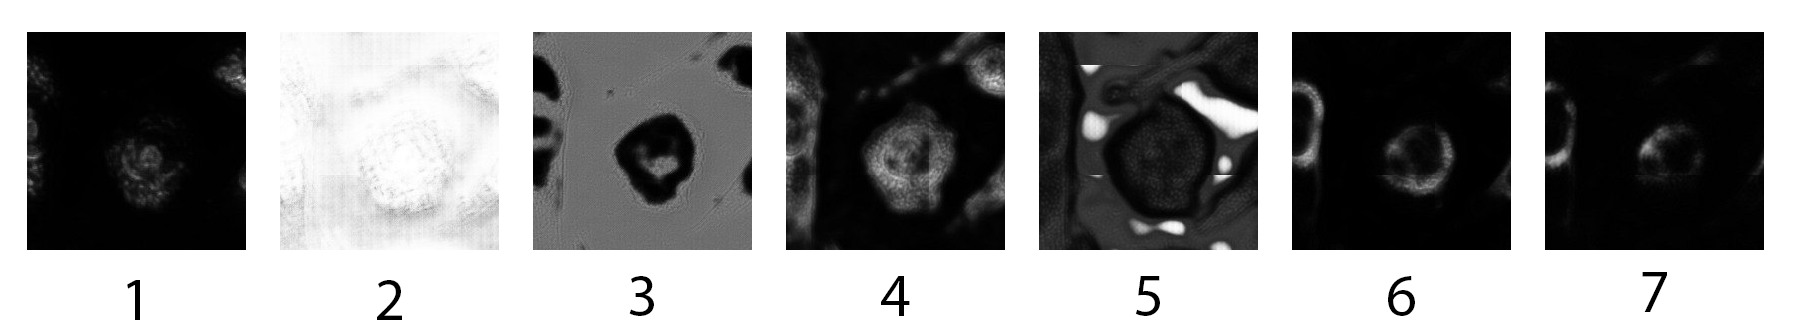
\includegraphics[width=\linewidth]{bilder/golgi/asymmetrical-predictions.png}
		\caption{Results of advanced versions of MSE training}\label{fig:golgi-asymmetrical-predictions}
	\end{center}
\end{figure} 
        \paragraph{Use of gradient in loss}
        \paragraph{Noise reduction methods}

    \pagebreak
    \subsection{GFP}
    Green fluorescent protein (GFP) is protein that produces bright green fluroescence from the whole cell surface. Some cells express this protein naturally, therefore there is no need to perform cell staining or fixation in this case and the imaging can be done on living cells. Fixation of the cells is a processes of destructing their membrane and fixing them on the plate in order for the stain antibody to be able to enter the cell. The difference in DIC imaging between fixed and not fixed cells is presented in Figure \ref{fig:fixed-not-fixed}. Clearly, cell membrane is intact and clearly defined in not fixed cells, whereas in not fixed ones there is almost no definite membrane present. 
    
    Nevertheless, in order to get training data for all other targets (nuclei, ER, Golgi apparatus) the staining procedure is unavoidable. And staining requires the cells first to be fixed. That brings up the limitation of current \textit{in silico} labeling research --- cells have to be fixated in any case. DIC imaging of living and fixed cells look very different and models trained on fixed cells do not generalize well to not fixed ones. Luckily, fixing cells is not a cumbersome lab procedure and is far easier than staining the cells, which is escaped with the help of \textit{in silico} fluorescence labeling. After successfull training of the model on living GFP expressing cells, we found out that other models cannot perform that well on living cells. Therefore, the cells were fixed in order to look alike with previously acquired data and the experiments were repeated. Nevertheless, we recommend to look into the possibilities of transfer learning from fixed to live cells. The results of training on the fixated cells are presented below. 
    
    For this experiment another cell phenotype was chosen --- H19. Training the model to predict GFP fluorescence essentially allows to predict the area of the whole cell, that is used in further downstream analysis. There is no need to capture the intensities as they do not bring any useful features for selection step in CLD. However they might help for algorithms like watershed to find separate cells in order to count them. Yet the task can be simplified to predicting binary mask of GFP signal too. Binarized images are well-suited for cell area predictions. Altough one has to find a corresponding image preprocessing pipeline in order to convert training intesity fluorescence imaging into masks first. Both tranining variations are provided in this chapter --- with and without prediction of the intensities. 
    \begin{figure}[H]
        \begin{center}
            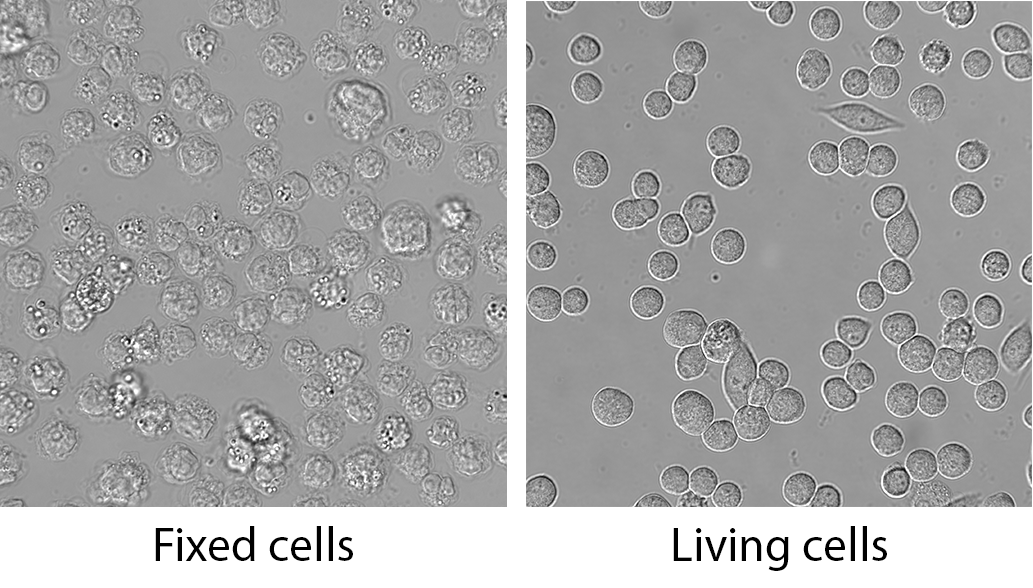
\includegraphics[width=0.5\linewidth]{bilder/gfp/fixed-not-fixed.png}
            \caption{Examples of fixed and not fixed cells DIC imaging}\label{fig:fixed-not-fixed}
        \end{center}
    \end{figure}
    \subsubsection{Preprocessing}
        \begin{figure}[H]
	\begin{center}
		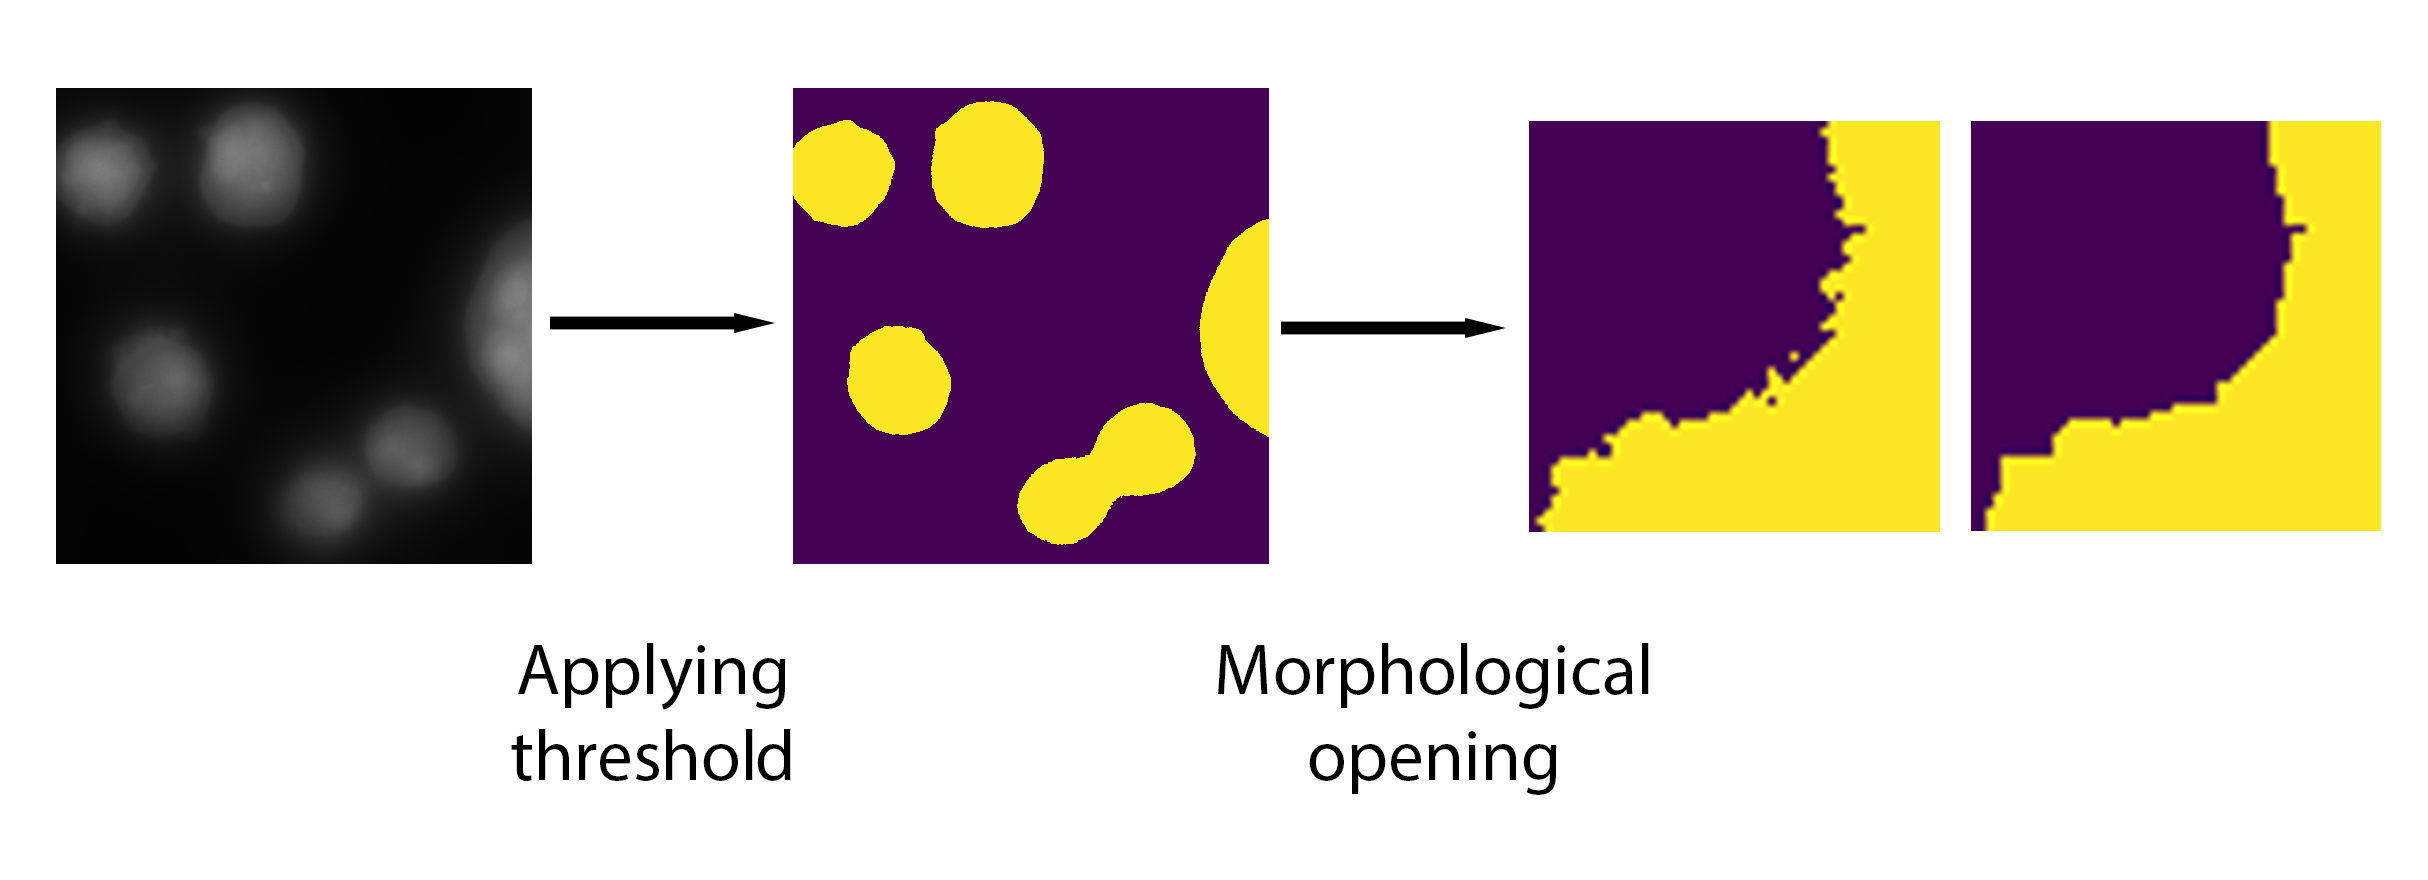
\includegraphics[width=0.5\linewidth]{bilder/gfp/binary-bce/preprocessing/preprocessing-gfp.png}
		\caption{Converting gfp to a binary mask}\label{fig:gfp-binary}
	\end{center}
\end{figure}

    \subsubsection{Predictions}
        Figure \ref{fig:gfp-pcc-predictions} presents the result of training with PCC loss on intensity images. The model convergence and visual comparison between ground truth and predictions is displayed. One can see that some of the cells are present in predictions, but are missing in ground truth images. These are dead cells that do not express GFP anymore, however the cell body is still present in DIC. Additional observation is that the boundary is generally blurry than in ground truth fluorescence, which is typical for all previous organelles as well. However all cells are clearly visible and can be separated using additional image postprocessing pipelines.
\begin{figure}[H]
	\begin{center}
		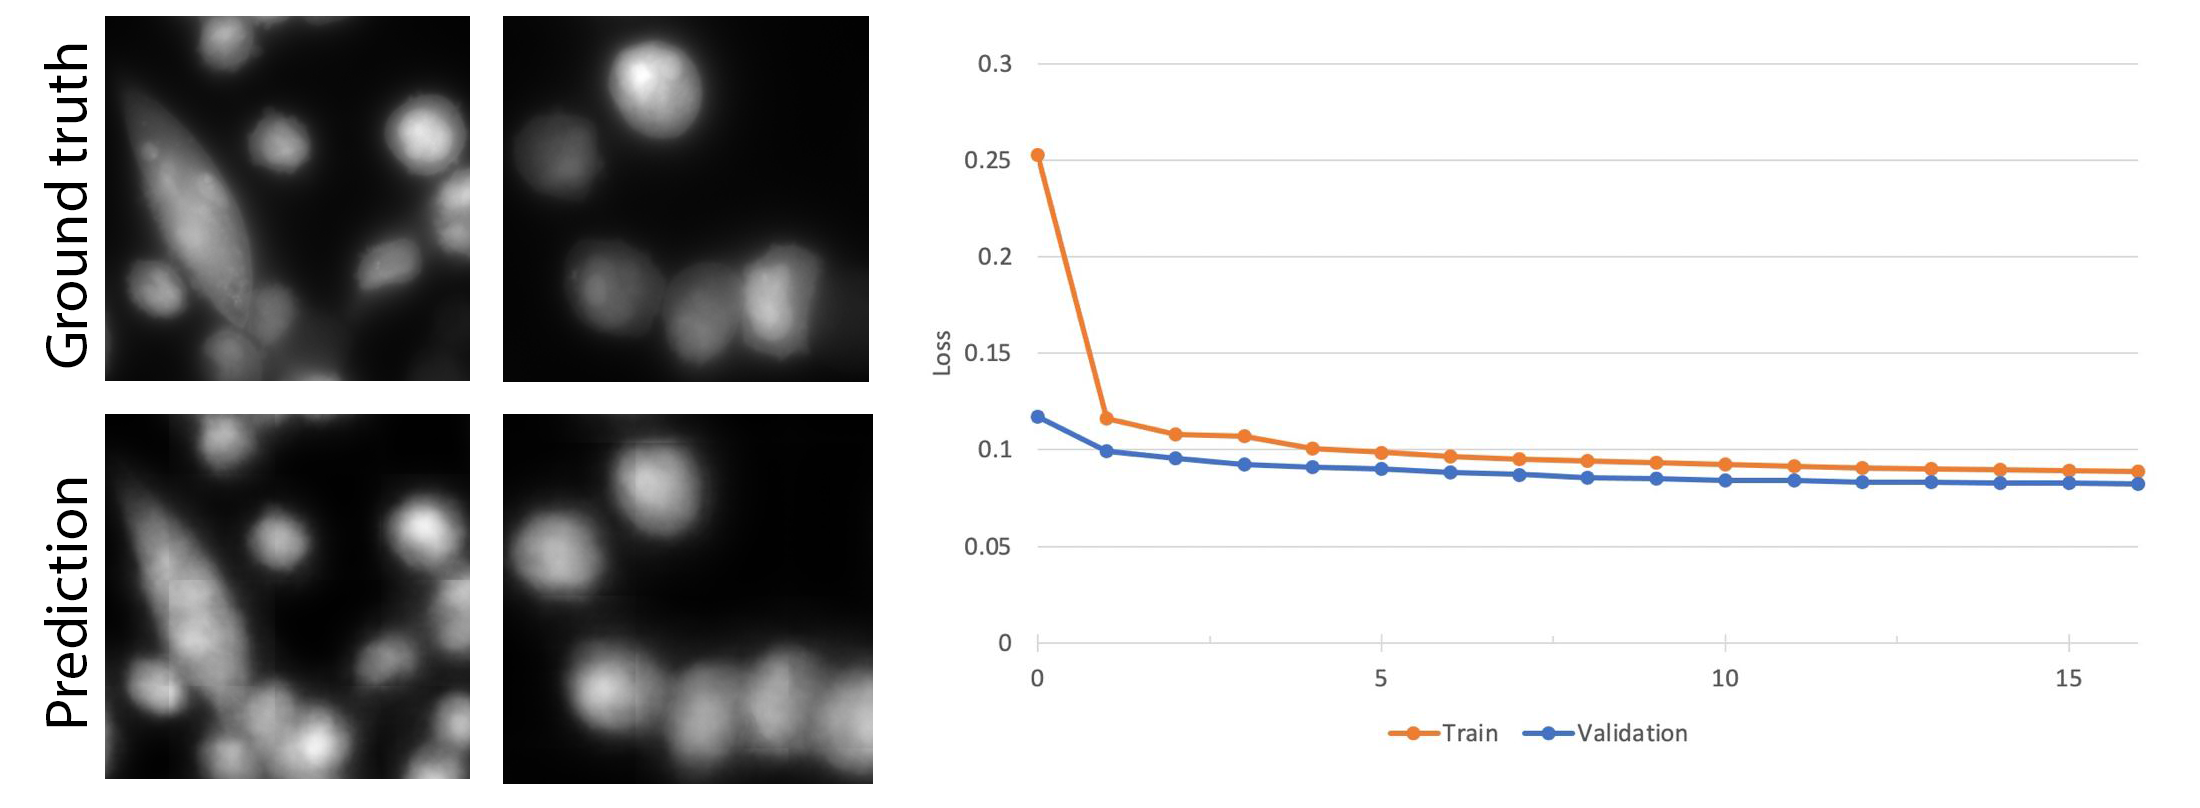
\includegraphics[width=0.9\linewidth]{bilder/gfp/predictions.png}
		\caption{Training with Pearson correlation loss}\label{fig:gfp-pcc-predictions}
	\end{center}
\end{figure}

In Figure \ref{fig:gfp-bce-predictions} one can find results of training on the binarized image dataset. Model does converge and predictions are successfull as well. Without the intensities it might be more difficult to visually separate the cells from the mask, rather then in the image with intensity values. The predicted masks are not binarized yet and contain continuous values from $[0, 1]$ interval. One can see how the model generalizes in the following observation: preprocessed ground truth image still has not very strict boundaries in its masking even after local thresholding binarization. After zooming in one can see that some cell's boundaries were oversegmented. This happens due to the different intensity values for different cells. However, this is not a an issue as the model is still able to generalize well and predicts the middle part of the cell confidently, then smoothly reduces the confidence on the cell boundary. After thresholding such predictions one can choose such a threshold that will get just enough of the cell boundary needed. In our case the value was chosen to be $0.8$.

An interesting detail here are dead cells mentioned above. They are present in DIC, but do not express GFP. One can see a clear example of such cells selected with green circles in Figure \ref{fig:gfp-bce-predictions}. The model generalizes in a way that it continues to segment all of the cells regardless of their state. This is an expected behavior as the amount of dead cells in the dataset is pretty low and ocasional mistakes do not push the model strongly enough to be able to learn the features that separate dead from alive cells. We proceed with the existing model to futher evaluation, however it might be useful for further research to address this issue. For example, \cite{Christiansen_2018} mentions the ability of their model to detect dead cells from alive by staning the dead ones and then traning the model to differentiate between them.

\begin{figure}[H]
	\begin{center}
		\includegraphics[width=0.7\linewidth]{bilder/gfp/binary-bce/enlarged.png}
		\caption{Training with BCE loss}\label{fig:gfp-bce-predictions}
	\end{center}
\end{figure}

    \subsubsection{Downstream metrics}
        TODO move to separate chapter?
        In this case only two metrics are important for evaluation --- the cell area and the cell count (see Table \ref{table:gfp-metrics}). Both Pearson correlation and Spearman rank coefficients are lower than in previous experiments. Influence of additional segmentation of dead cells by the model lowers correlation scores, however they still signalize the presence of a strong correlation between prediction and ground truth. 
\begin{table}[H]
    \centering
    \caption{Correlation coefficients for practical biological evaluation}
        \begin{adjustbox}{width=0.4\textwidth}
            \begin{tabular}{|c|c|c|}\hline
                BCE loss&Pearson&Spearman
                \\\hline\hline
                Number of ER&0.67&0.64\\\hline
                Area&0.82&0.75\\\hline
            \end{tabular}
            \label{table:gfp-metrics}
        \end{adjustbox}
\end{table}

Violin and scattter plots depicting the two above mentioned metrics are shown in Figure \ref{fig:gfp-bce-metrics}.
\begin{figure}[H]
	\begin{center}
		\includegraphics[width=\linewidth]{bilder/gfp/binary-bce/gfp-bce-metrics.png}
		\caption{Biological metrics}\label{fig:gfp-bce-metrics}
	\end{center}
\end{figure}
    \subsubsection{Combination of GFP, nuclei and ER}
        Now having three successful models that are able to predict GFP fluorescence from the whole cell, nuclei and ER, one can combine their predictions for the same image. To do that an output RGB image was constructed, where each prediction takes one channel. The resulting image is shown in Figure \ref{fig:combined}. Additionally one can see that the GFP model has successfully generalized on other cell phenotypes (CHOZN, PHX). Originally this model was trained on H19 phenotype only, however predictions for two other phenotypes (see Figure  \ref{fig:combined} PHX, CHOZN) highlight the cell area successfully as well.

\begin{figure}[htb]
	\begin{center}
		\includegraphics[width=0.85\linewidth]{bilder/combined/combined.png}
		\caption[GFP, Nuclei and ER combined]%
		{Combination of predictions of three UNets: GFP, nuclei and ER. Each organelle occupies one RGB channel: red --- ER, green --- GFP, blue --- nuclei.}\label{fig:combined}
	\end{center}
\end{figure}

    \subsubsection{Conclusions}
        GFP \textit{in silico} fluorescence labeling can successfully be used for counting the number of cells and estimating their size. The created models can both predict the intensity images as well as binarized masks. Intensity predictions might be more useful for the number of cells estimation as the cells better visually separate there. The models were evaluated on two biological metrics: cell size and cell count. The correlation coefficient suggests a strong correlation between the predictions and ground truth. 

The model has limitations in its ability to differentiate between dead and alive cells. This issue should be addressed in further reasearch after acquiring data for labeling dead cells. Despite the difficulty to clearly determine cell boundaries during image preprocessing for fluorescence image binarization (its overpredicting in some cases) the model can successfully generalize and predict a correct boundary for all cells. The images of not fixed cells were provided for the first time during GFP experiments and it was clear that previously trained models do not generalize on them well.  Because of this the limitation of research in terms of the cell fixation need was determined. However, it is recommended to look into possible transfer learning approaches get rid of the fixation step completely.
  

    \pagebreak
    \subsection{Model evaluation}
    \subsubsection{Metrics for downstream tasks}
        \begin{figure}[H]
	\begin{center}
		\includegraphics[width=\linewidth]{bilder/nuclei/metric/combined-metrics.png}
		\caption{Metrics for downstream tasks on nuclei}\label{fig:nuclei-downstream-metrics}
	\end{center}
\end{figure}

\begin{table}[H]
    \centering
    \caption{Correlation coefficients for downstream tasks}
        \begin{adjustbox}{width=0.4\textwidth}
            \begin{tabular}{|c|c|c|}\hline
                &Pearson&Spearman
                \\\hline\hline
                Number of nuclei&0.995&0.994\\\hline
                Total intensity&0.902&.911\\\hline
                Mean intensity&0.907&0.904\\\hline
                Area&0.992&0.990\\\hline
            \end{tabular}
        \end{adjustbox}
\end{table}

    \subsubsection{Influence of different loss functions on metrics for downstream tasks}
